%\chapter{EvoGraph: A High Performance Accelerator-Based Framework for Processing Evolving Graphs}
\chapter{EvoGraph: Processing Evolving Graphs on Accelerator-Based Systems}
%\section{Introduction}

%High performance machines are increasingly using GPUs~\cite{15, 16, 17, 18, 19}, to leverage their scalability and low dollar to FLOPS ratios.  As a result, GPUs have become the main compute engines for today’s HPC clusters and supercomputers like Titan in Oak Ridge~\cite{titan}. This trend continues with the move toward exascale machines that are expected to be comprised of millions of accelerator and general purpose cores, whether packaged as `thin' or `fat' nodes. 
As discussed in last chapter, a recent trend is the gain in popularity of GPU processing in many domains such as social networks, e-commerce, advertising, and genomics. This has motivated the growing interest in large-scale real-world graph processing for both scientific and commercial applications, as well as the recent efforts in accelerator-based graph processing frameworks such as MapGraph~\cite{mapgraph}, Medusa~\cite{medusa}, CuSha~\cite{cusha}, GraphReduce~\cite{GraphReduce}, and so on. An important aspect of real-world graphs, like Facebook friend lists or Twitter follower graphs, is that they are dynamic.  Given the billions of Facebook~\cite{linkbench} users sharing more than 100 billion photos and posts per month, let alone the volume on Twitter~\cite{twitter} or other blogging platforms, there is a huge need to quickly analyze this high velocity stream of graph data. 

However, state-of-the-art graph analytics for dynamic graphs follow a store-and-static-compute model that involves batching these updates into discrete time intervals, applying all of the updates to the total graph, and then rerunning the static analysis.  There is considerable redundancy and inefficiency in this approach to analyzing this \textit{evolving} graph sequence.  Static graph analytics on a single version of the evolving graph, even when leveraging massive amount of parallelism offered by thousands of cores in a GPU, can be very slow due to the extreme scale of many real-world graphs (e.g., one Facebook graph purportedly has a trillion edges~\cite{fb}) and/or because of the complexity of the graph queries that are traditionally both compute and memory intensive. Second, data movement of the entire input graph repeatedly between the host and the GPU over the slow PCIe link can result in substantial overhead, which in turn can overshadow the benefits from the massive parallelism offered by a GPU.  Finally, there are real world graph analytics problems that inherently require soft or hard real-time guarantees, e.g., real-time anomaly detection, disease spreading, etc, and hence can't use the traditional static recomputation model. Beyond just hardware performance, we also note that the skills to write performant GPU code are substantially different from the coding skills that many analysts have learned.  As one can therefore see, the many demands of high velocity graph data, both commercial and scientific, have outstripped the traditional, batched static graph analytics models, even when using GPUs.

To address this, we propose a two-pronged approach to deal with both the performance and programmability challenges. We introduce an accelerator-based incremental graph processing framework called EvoGraph. EvoGraph employs a new variant of  the popular Gather-Apply-Scatter (GAS) programming model, which we call Incremental-GAS (or I-GAS), to incrementally process a batched stream of updates (i.e., edge/vertex insertions and deletions).  The key insight is that I-GAS algorithms are designed to work over a (dynamically determined) sub-graph of the previous version of the evolving graph.  For many popular graph algorithms and real-world graphs, the corresponding I-GAS logic affects only a fractional portion of the graph; this reduction in problem size can result in tremendous performance benefits compared to static recomputation of the graph algorithm on the entire graph.  The modest additions of the I-GAS model to the already-published GAS model interface enable an easy transition of analysts from coding in a static to a dynamic streaming environment.

From a simplistic view, it would seem that incremental methods would always be preferable.  However, there are scenarios when a streamed update may affect a very large portion of the graph, and incremental processing won't help much or may even be worse than static recomputation due to overheads of incremental execution. One such counterexample is in the incremental version of Breadth First Search (BFS), where updates that affect vertices close to the source/root node will affect nearly the entire BFS tree. Here the incremental run can at best perform as good as the static re-run, and may even be worse. Note that this is not a concern about correctness of the result, but over performance.  Therefore, in order to handle such scenarios, we employ a \textit{per batch}, property-based dynamic choice between incremental and static graph processing called \textit{‘property-guard’}. Utilizing user-defined and built-in properties (e.g., vertex degree) along with programmable control policies, EvoGraph analyzes each update batch and dynamically decides whether to process the graph incrementally using I-GAS or to fall back to static recomputation. 

This chapter makes the following technical contributions:
\begin{itemize}
 \item \textit{EvoGraph}, an accelerator-based high-performance incremental graph processing framework, built on top of GraphReduce~\cite{GR}, to process evolving graphs by avoiding the naive static graph recomputation approach. User's sequential code for incremental graph algorithms in EvoGraph are seamlessly mapped to GPU for acceleration. 
 \item Improved GPU core utilization via dynamic merging of GPU contexts from different graph applications, and additional hardware parallelism extracted using deep copy operations on separate CUDA streams to leverage the multiple hardware queues (Hyper-Qs) in GPUs.
 \item An extensive evaluation of 3 popular graph algorithms on real-world and synthetic graph datasets show that EvoGraph can significantly outperform the existing static recomputation approach. Compared to competitive frameworks like STINGER, EvoGraph achieves a speedup of up to 232x and overall throughput of 429 million updates/sec.
 \item Graph-property-based performance optimization called \textit{property-guard} to dynamically decide between static and dynamic graph execution based on user-defined and built-in graph properties, resulting in a speedup of up to 18.4x over a naive streaming approach.  
\end{itemize}

The remainder of the chapter is organized as follows: Section 4.1 discusses the motivation and challenges of evolving graph analytics. Section 4.2 dissects the design choices. Section 4.3 introduces our EvoGraph runtime framework. Section 4.4 highlights case study of three classes of incremental graph algorithms implemented using EvoGraph. Section 4.5 presents the experimental setup and result analysis followed by conclusions and future work. 

%\section{Background And Motivation}

%\subsection{Gather-Apply-Scatter Model}

%As introduced in the previous work ~\cite{pregel}, ~\cite{powergraph}, ~\cite{graphlab}, ~\cite{GraphReduce}, the Gather-Apply-Scatter (GAS) computation model has been widely adopted in research and industry to simply and effectively express a broad range of graph algorithms.  Under GAS, the input data can be  described as a directed graph, $G = (V, E)$, where $V$ denotes the vertex set and $E$ denotes the directed edge set. A vertex value is associated with each $v\in V$, and each directed edge $e_{ij}$ is associated with 
%a source vertex $u$ and a target vertex $v$: $e_{ij} =(u, v) \in E$. A GAS-based computation iterates over three sequential phases, the eponymous \textit{Gather}, \textit{Apply} and \textit{Scatter}.  The iteration process continues until the vertex state no longer changes. In the Gather phase, in-coming messages are processed and combined (reduced) into one message. In the Apply phase, vertices use the combined message to update their states. Finally, in the Scatter phase, vertices can send a message to their neighbors along their edges. Note that although it is proven to be effective to process static graphs, GAS model has not been applied to process constantly-evolving dynamic graphs. We will discuss this challenge next. 

%\section{Motivation and Challenges of Processing Evolving Graphs On GPU}
\section{Motivation and Challenges}
\begin{figure}[!t]
\centering
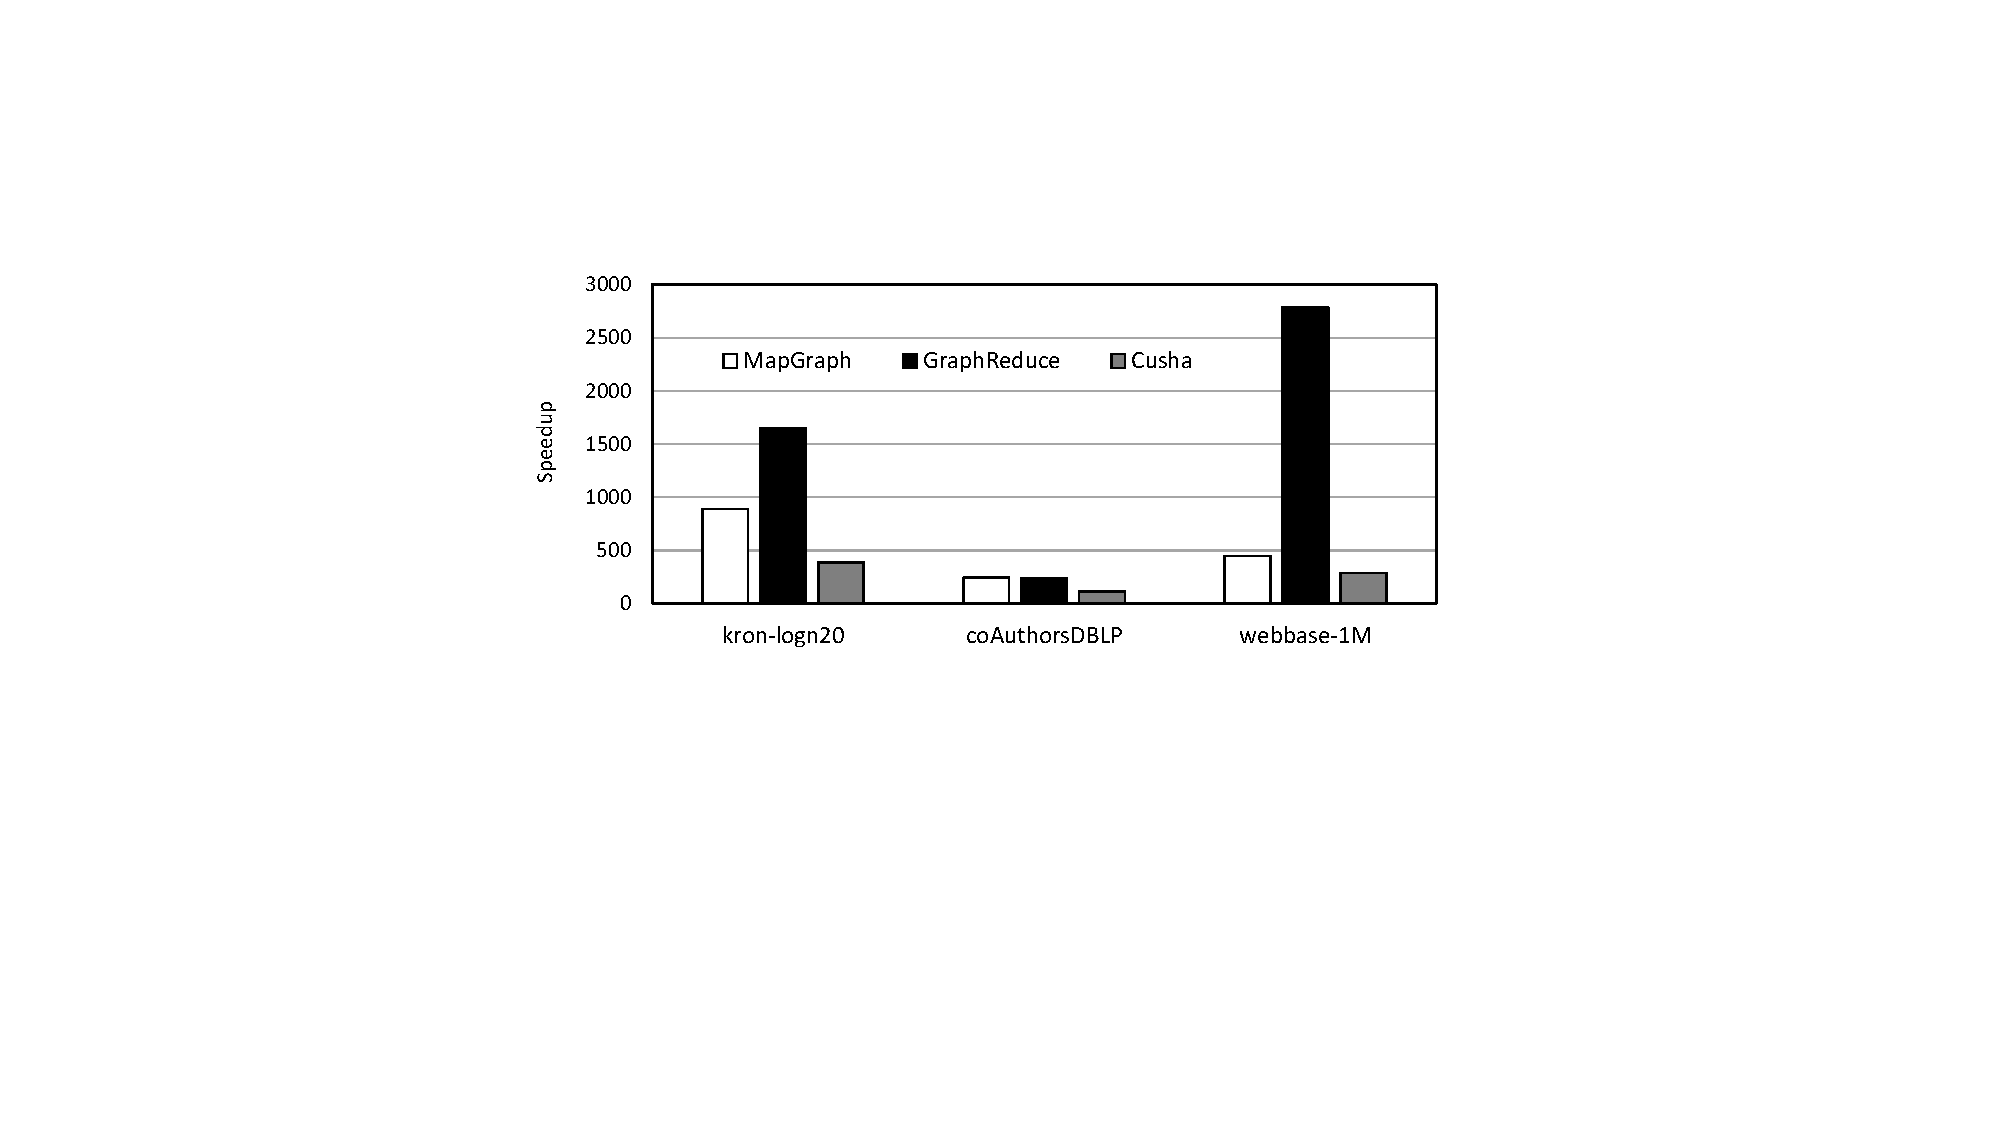
\includegraphics[width=0.75\textwidth,height=0.75\textheight,keepaspectratio]{figures/static_GR.pdf}
\caption{State-of-the-art GPU frameworks (i.e., MapGraph, GraphReduce and Cusha) for processing static graphs significantly outperform the best CPU-based framework X-Stream (baseline).}
\label{fig:static}
%\vspace{-0.5\baselineskip}
\end{figure}




%GPU has emerged as one of the most powerful computation accelerators for world-class supercomputers [] because of its unparalleled massive amount of parallelism and ability to speedup a wide range of HPC applications. Compared to its counterpart CPU, it also often provides superior acceleration for general graph algorithms. Figure \ref{fig:static} demonstrates that for processing three real-wold in-memory \textit{static graphs} under BFS, state-of-the-art GPU frameworks outperform the best CPU-based graph analytics (i.e., X-Stream) by an average speedup of 782x and up to 2785x (i.e., GraphReduce on \textit{webbase-1M}). This motivates us to unleash GPU's high computation power for processing \textit{evolving dynamic graphs}. 
%
%
%
%
%
%Figure \ref{fig:link} shows an example of an evolving Linkedin social network graph, in which a subgraph (circled by red dash line) is going through \textit{update batches} (e.g., insert:(1,4) and delete:(1,3)) at different time point. Different colors of dots represent work fields. Processing such common constantly-evolving social network graphs on GPUs is very challenging because (i) highly efficient computation model and convenient programming constructs do not exist for programmers to effectively express their algorithms on GPUs, (ii) how to efficiently utilize the parallelism provided by GPUs to deal with the computation and data storage overlap in dynamic graphs is complicated, and (iii) how to extract the most throughput from GPUs without burdening the users with hardware details is unclear. In order to address these challenges, we propose a runtime graph analytics framework named \textit{EvoGraph} to process complex evolving graphs on modern GPUs. Under EvoGraph, users only need to write sequential codes and the sophisticated runtime will seamlessly map the incremental graphs to GPU for acceleration. We will discuss the design details of EvoGraph next. 
%
%
%
%\begin{figure}[!t]
%\centering
%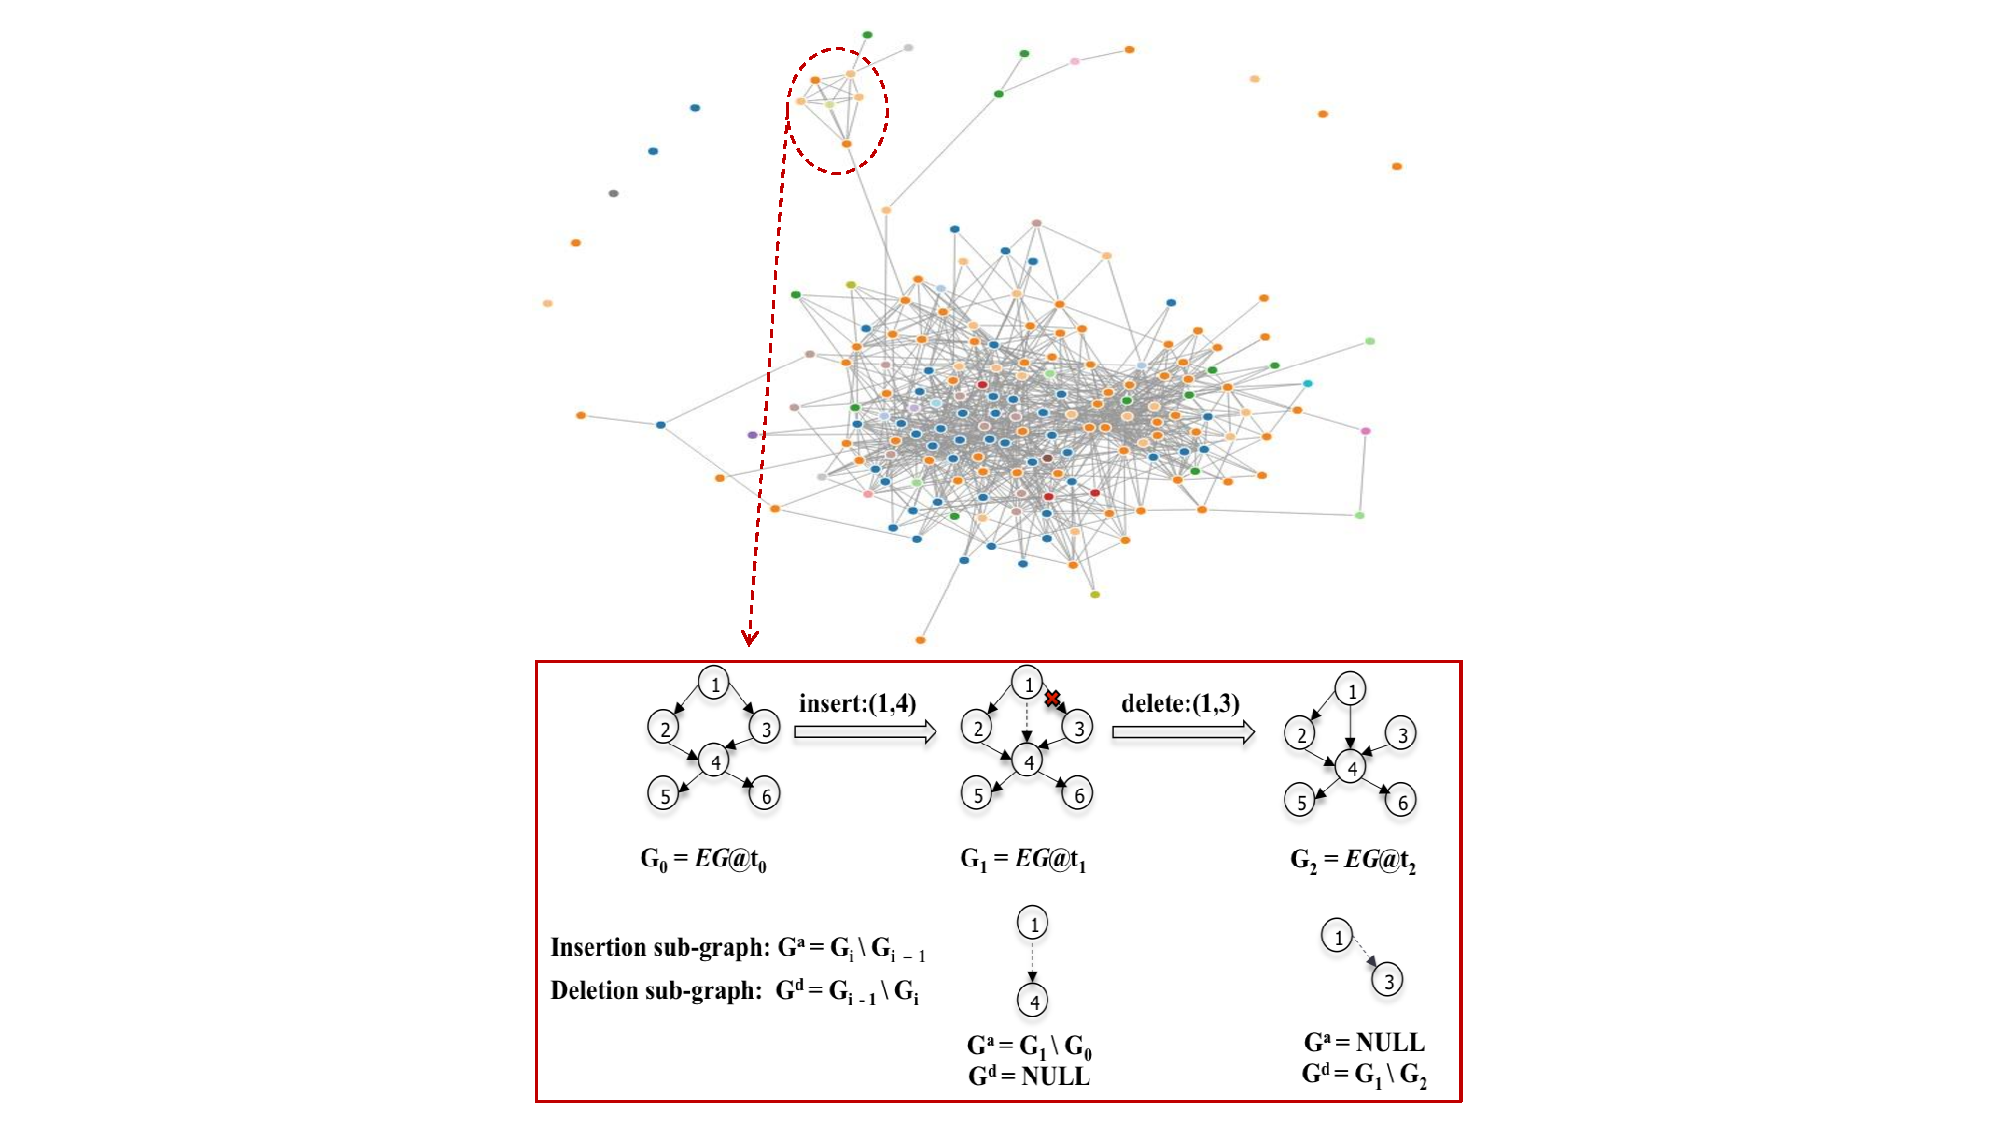
\includegraphics [width=1\columnwidth]{figures/link.pdf}
%\caption{A subgraph of a Linkedin social network has been updated over time but the rest of the network remains the same. }
%\label{fig:link}
%\vspace{-0.5\baselineskip}
%\end{figure}


GPUs have emerged as one of the most powerful computation accelerators for world-class supercomputers~\cite{titan} because of their unparalleled massive amount of parallelism and ability to speedup a wide range of HPC applications. Compared to its counterpart CPU, it also often provides superior acceleration for general graph algorithms. Figure \ref{fig:static} demonstrates that for processing three real-wold in-memory \textit{static graphs} under BFS, state-of-the-art GPU frameworks outperform the best CPU-based graph analytics (i.e., X-Stream) by an average speedup of 782x and up to 2785x (i.e., GraphReduce on \textit{webbase-1M}). This motivates us to unleash GPU's high computation power for processing \textit{evolving dynamic graphs}. 

Figure \ref{fig:link} shows an example of an evolving Linkedin social network graph, in which a subgraph (circled by red dashed line) is going through \textit{update batches} (e.g., insert:(1,4) and delete:(1,3)) at different time point. Different colors of dots represent work fields. Processing such common constantly-evolving social network graphs on GPUs is very challenging because (i) highly efficient computation model and convenient programming constructs do not exist for programmers to effectively express their algorithms on GPUs, (ii) how to efficiently utilize the parallelism provided by GPUs to deal with the computation and data storage overlap in dynamic graphs is complicated, and (iii) how to extract the most throughput from GPUs without burdening the users with hardware details is unclear. In order to address these challenges, we designed a runtime graph analytics framework named \textit{EvoGraph} to process complex evolving graphs on modern GPUs. Under EvoGraph, users only need to write sequential codes and the sophisticated runtime will seamlessly map the incremental graphs to GPU for acceleration. We will discuss the design details of EvoGraph next. 



\begin{figure}[!t]
%\vskip -3 mm
\centering
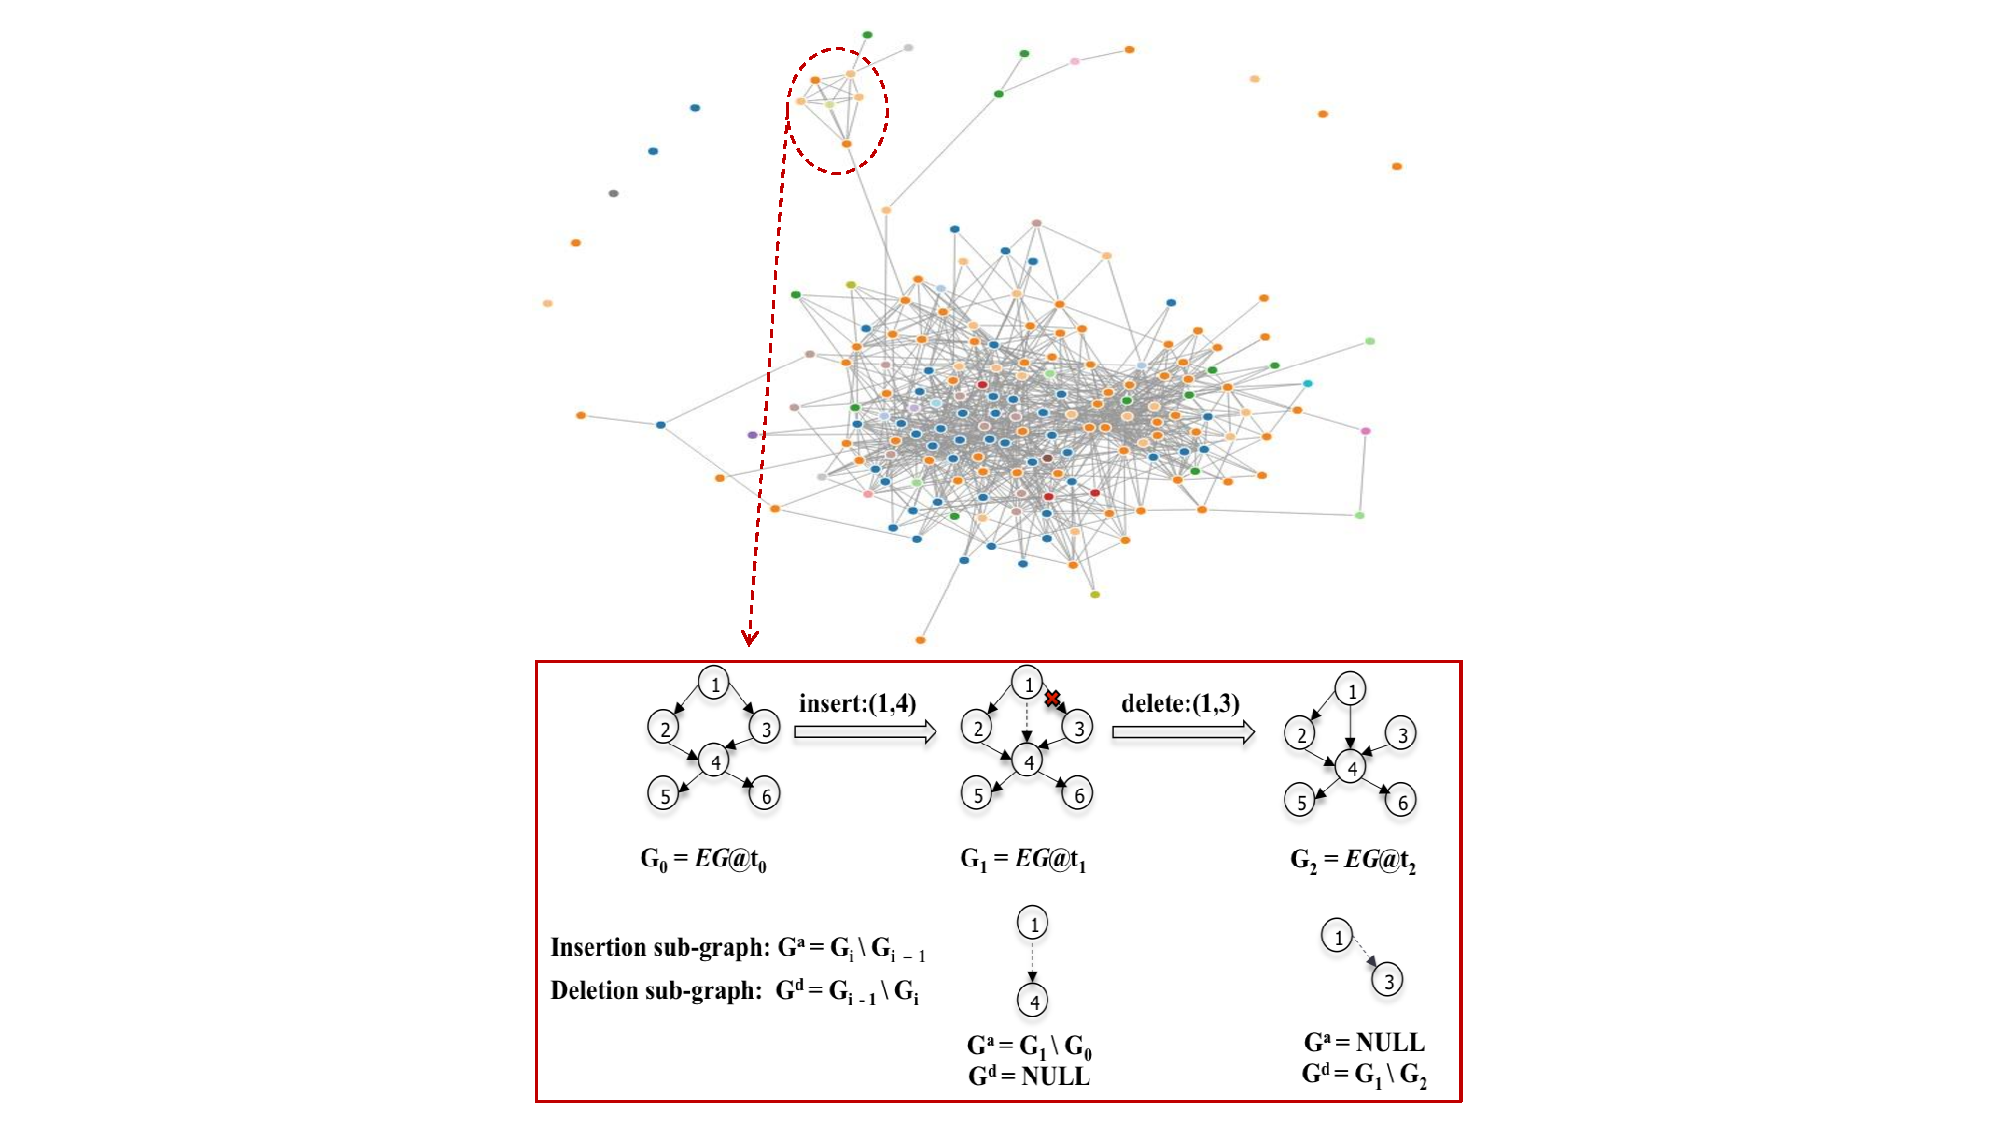
\includegraphics [width=1\columnwidth]{figures/link.pdf}
\caption{A subgraph of a Linkedin social network has been updated over time but the rest of the network remains the same. }
\label{fig:link}
%\vspace{-0.5\baselineskip}
%\vskip -3 mm
\end{figure}



\section{Design Choices}

%In general, there are two major strategies for processing evolving graphs: (1) Offline evolving graph processing where multiple versions of the graph are stored and analyzed to observe the change in certain graph properties over time. (2) Online evolving graph processing that involve real-time continuous query processing over streaming updates on the evolving graph. EvoGraph is a framework designed for online graph analytics. 
%
%Broadly, there are three key characteristics of evolving graphs that dictate the design decisions for EvoGraph: 
%
%
%\begin{itemize}
%  \item Computation overlap in a sequence of versions
%  \item Data or working set overlap in a sequence of versions
%  \item Choice between static and dynamic execution runtime
%\end{itemize}
%
%\subsection{Computation Overlap and Programming Model}
%
%Shown in Figure \ref{fig:link}, across multiple versions or snapshots of an evolving graph, the vertex states or values for many vertices remain the same over time, and thus their recomputation is essentially redundant. We define an \textit{inconsistent vertex} as a vertex for which one or more properties are affected when an update batch is applied. For instance, when calculating out-degree of vertices, an insertion or deletion of edge ($v_i$,$v_j$) only makes vertex $v_i$ inconsistent. However, under BFS (Breadth-First Search) algorithm, insertion of edge ($v_i$,$v_j$) makes $v_j$ and all the vertices that are descendants of $v_j$ \textit{inconsistent}. One can consider the entire vertex set $V$ to be inconsistent by default. But for many real-world evolving graphs (e.g., Linkedin or Facebook social network), changes affect only a very small subset of the graph. Therefore, computing the vertex states only for those inconsistent vertices while maintaining the vertex states for the rest will significantly reduce the computation time. Because of this,  we propose \textbf{I-GAS} programming model based on the classic GAS abstraction (Section 4.1) for incremental graph processing, which will be discussed in detail in Section 4.3. To reduce overheads, I-GAS builds a group of inconsistent vertex sets and sub-graphs that are affected by an update batch and then reduce the incremental graph problem to a sub-problem under GAS.
%
%
%\subsection{Working Set Overlap and Data Structure Choice}
%
% Another key observation to make here is that there can be a huge overlap in the edge and vertex sets between consecutive versions of an evolving graph. For instance, if a graph evolved from G to G' during a certain time epoch t and let $\delta1 = G'-G$ (insertions), $\delta2 = G-G'$ (deletions) then $G \cap G' = G- \delta2 = G' - \delta1$ is the overlap between the working sets of the two consecutive versions. 
%
%Furthermore, there are multiple options for choosing data structure to store an evolving graph. Assume the graph has $n$ vertices and $m$ edges at certain time point. \textit{Adjacency matrices} allow fast update (i.e., $O(1)$ time cost) with both insertions and deletions but require $O(n^2)$ space. \textit{Adjacency lists} are space efficient ($O(m+n)$) and allow fast update, but graph traversals are very inefficient due to non-contiguous memory nodes in the adjacency edge list. \textit{Compressed Sparse Row} (CSR) formats provide both space efficiency and fast traversal through storing offsets rather than all the valid fields in the adjacency matrix. But its insertion and deletion are very expensive because each update requires shifting of the graph data throughout the compressed array to match the compressed format. In order to allow faster updates to the graph and process both the incremental and static graph algorithms efficiently, EvoGraph uses a hybrid data structure: edge-lists to store incremental updates and compressed format to store the previous static version of the graph. As mentioned above, the edge-list will allow faster updates without adversely affecting the performance of incremental computation. Meanwhile, the compressed matrix format allows faster parallel computation over the static version of the graph. EvoGraph merges the update list and the static graph whenever required (see Section 4.3 for details).
%
%
%\subsection{Static vs. Dynamic Runtime}
%
%Runtime of online graph analytics varies widely depending on the algorithm and the update list. On one hand, there are cases in which incremental algorithms affect only a small local portion of the entire graph (e.g., making a small subset of the graph inconsistent). As demonstrated in [3, 4, 26], per-vertex properties that depend on a fixed radius affect only a local portion of the graph and hence the runtime is proportional to the update batch size (e.g., for triangle counting and in-edge calculation). On the other hand, there are classes of incremental algorithms whose properties depend on the graph path which may cause a large portion of the graph to be inconsistent, resulting in a complete recomputation of the graph. Under this scenario, incremental processing will not achieve any performance benefit over static recomputation and might even suffer from a performance degradation due to the overheads associated with the incremental execution. To effectively handle both scenarios,  EvoGraph applies a heuristic to select the execution pathway: incremental or static.  The decision is made dynamically based on a set of built-in or user-defined graph property checks (e.g., vertex degree information) and the fraction of inconsistent vertices in the update batch that meet the criteria. More specifically, if the update is predicted to affect a small portion of the graph then the incremental execution path is taken. Otherwise, the update is merged with the static graph, which will be then recomputed.  Take BFS for example. If 90\% of the inconsistent vertices in an update batch are of high degree, a large portion of the graph is likely to be impacted, so the static execution path will be taken. The metadata that is used to make decisions on execution path will be discussed in Section 4.3.
%
%
%\subsection{Context Merging and Multi-Level GPU Sharing}
%
%As mentioned previously, some incremental graph computation only affects a small portion of the graph and hence the GPU cores can be significantly underutilized. This gives us opportunities for GPU resource sharing among static and incremental graph computation. For NVIDIA GPUs, since the CUDA runtime does not allow more than one host processes to share the same GPU context (protection domain), the GPU workloads of two different applications cannot run concurrently on a single GPU. When processing incremental graphs, this could result in high context switching overhead and potential core idling. To avoid this, EvoGraph packs different application contexts into a single protection domain [7] (we call it `context merging'). Specifically, all the graph applications (static and incremental) collocated on a GPU are mapped to separate host threads of the same per GPU host process, with their respective GPU operations invoked via separate CUDA streams. Using this single GPU context to host all applications enables the cross-application sharing of GPU resources – a true multi-tenancy. Additionally, a specific advantage by leveraging CUDA streams is that all three GPU engines, (a) memory copy from host to device (H2D), (b) from device to host (D2H), and (c) computation, can be concurrently executed by different applications. Moreover, graph operations from different applications can also run concurrently on GPU, thereby achieving the benefits of space and time sharing. 
%
%\begin{figure}[!t]
%\centering
%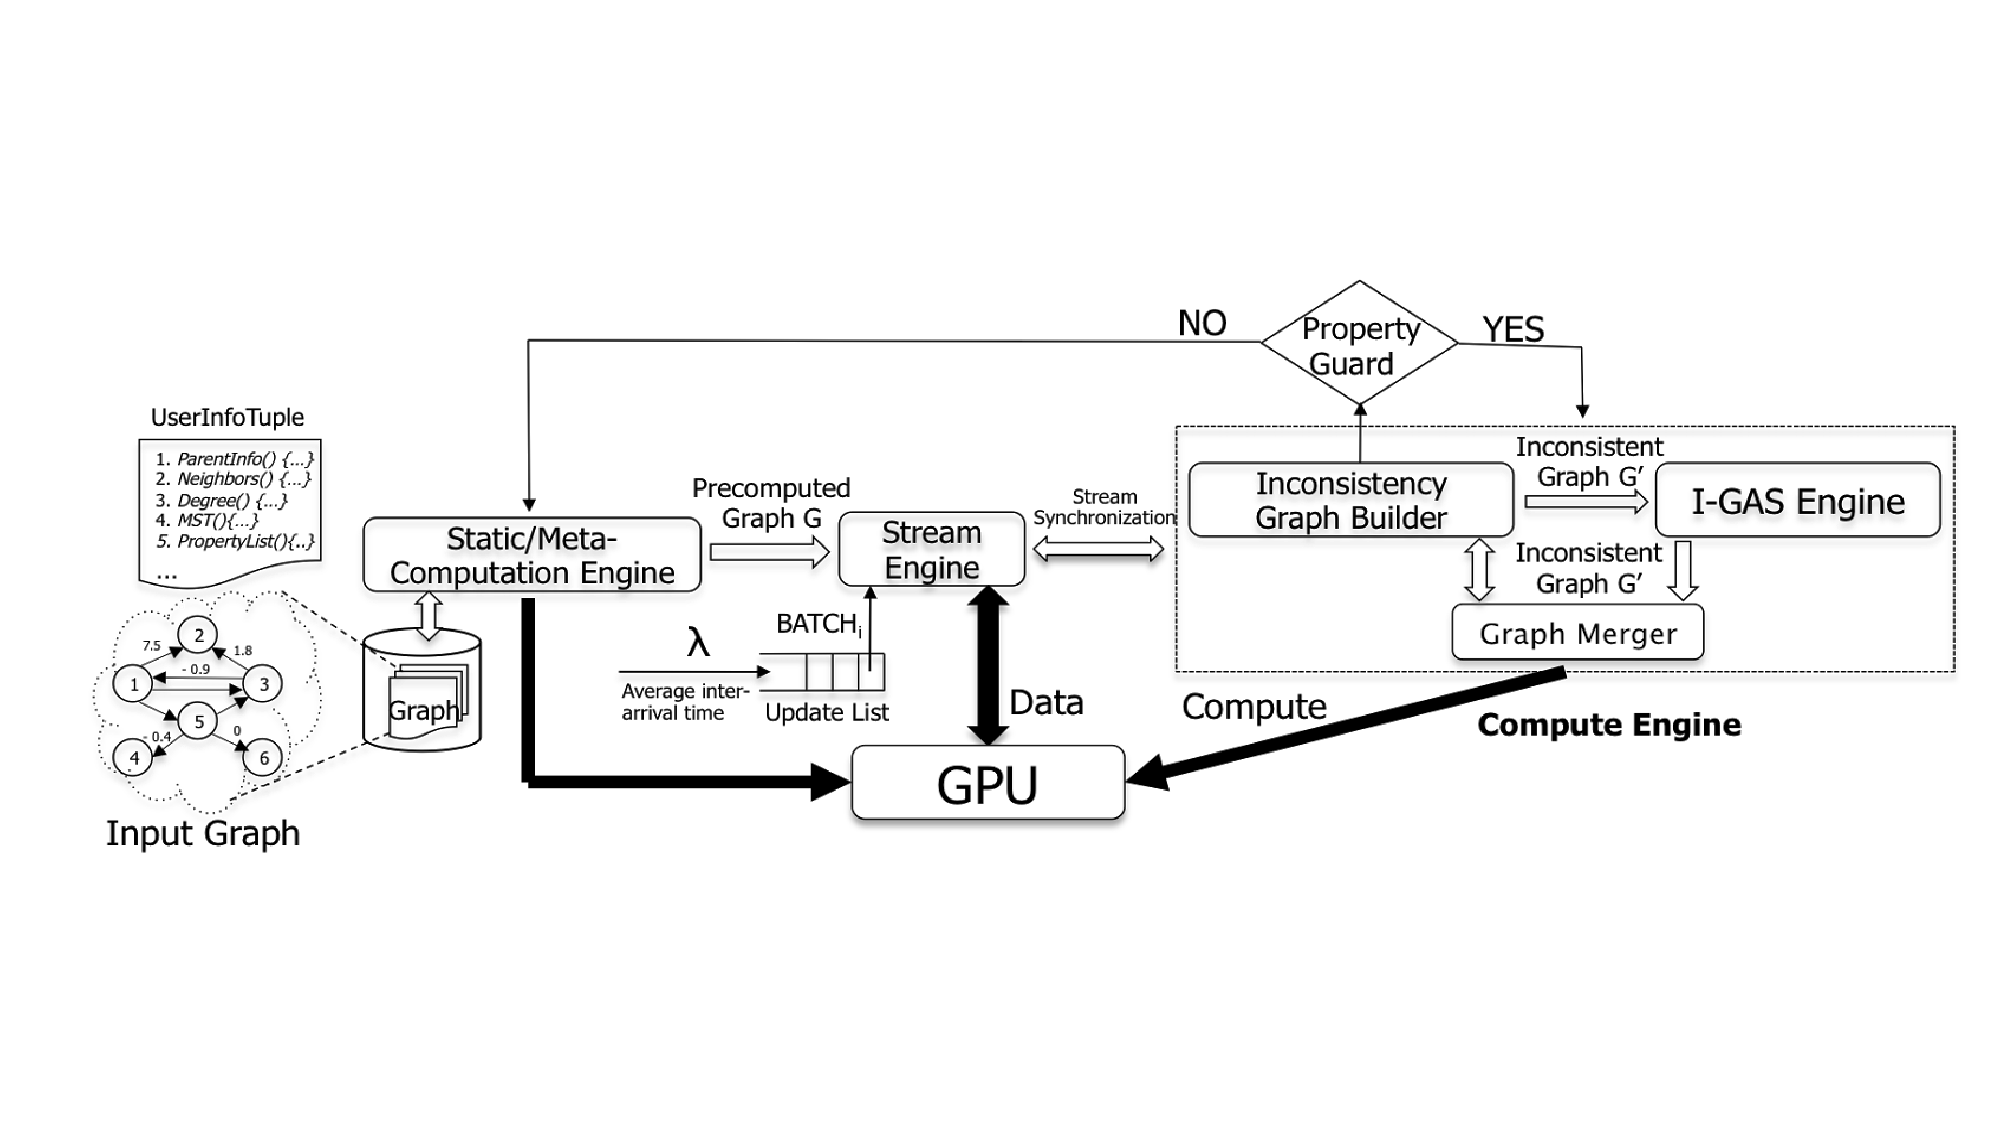
\includegraphics[width=1\columnwidth]{figures/framework.pdf}
%\caption{The software architecture diagram of EvoGraph.}
%\label{fig:framework}
%\vspace{-0.5\baselineskip}
%\end{figure}
%
%
%


In general, there are two major strategies for processing evolving graphs: (1) Offline evolving graph processing where multiple versions of the graph are stored and analyzed for the change in certain graph properties over time. (2) Online evolving graph processing that involve real-time continuous query processing over streaming updates on the evolving graph. EvoGraph is a framework designed for the latter. 

Broadly, there are three key characteristics of evolving graphs that dictate the design decisions for EvoGraph: 


\begin{itemize}
  \item Computation overlap in a sequence of graph versions
  \item Data or working set overlap in a sequence of graph versions
  \item Choice between static and dynamic execution runtime
\end{itemize}

\subsection{Computation Overlap and Programming Model}

Shown in Figure \ref{fig:link}, across multiple versions or snapshots of an evolving graph, the vertex states or values for many vertices remain the same over time, and thus their recomputation is essentially redundant. We define an \textit{inconsistent vertex} as a vertex for which one or more properties are affected when an update batch is applied. For instance, when calculating out-degree of vertices, an insertion or deletion of edge ($v_i$,$v_j$) only makes vertex $v_i$ inconsistent. However, under BFS (Breadth-First Search) algorithm, insertion of edge ($v_i$,$v_j$) makes $v_j$ and all the vertices that are descendants of $v_j$ \textit{inconsistent}. One can consider the entire vertex set $V$ to be inconsistent by default. But for many real-world evolving graphs (e.g., Linkedin or Facebook social network), changes affect only a very small subset of the graph. Therefore, computing the vertex states only for those inconsistent vertices while maintaining the vertex states for the rest will significantly reduce the computation time. Because of this,  we propose \textbf{I-GAS} programming model based on the classic GAS abstraction (Section 4.1) for incremental graph processing, which will be discussed in detail in Section 4.3. To reduce overheads, I-GAS builds a group of inconsistent vertex sets and sub-graphs that are affected by an update batch and then reduce the incremental graph problem to a sub-problem under GAS.


\subsection{Working Set Overlap and Data Structure Choice}

 Another key observation to make here is that there can be a huge overlap in the edge and vertex sets between consecutive versions of an evolving graph. For instance, if a graph evolved from G to G' during a certain time epoch t and let $\delta1 = G'-G$ (insertions), $\delta2 = G-G'$ (deletions) then $G \cap G' = G- \delta2 = G' - \delta1$ is the overlap between the working sets of the two consecutive versions. 

Furthermore, there are multiple options for choosing data structure to store an evolving graph. Assume the graph has $n$ vertices and $m$ edges at certain time point. \textit{Adjacency matrices} allow fast update (i.e., $O(1)$ time cost) with both insertions and deletions but require $O(n^2)$ space. \textit{Adjacency lists} are space efficient ($O(m+n)$) and allow fast update, but graph traversals are very inefficient due to non-contiguous memory nodes in the adjacency edge list. \textit{Compressed Sparse Row} (CSR)~\cite{csr} formats provide both space efficiency and fast traversal through storing offsets rather than all the valid fields in the adjacency matrix. But its insertion and deletion are very expensive because each update requires shifting of the graph data throughout the compressed array to match the compressed format. In order to allow faster updates and process both the incremental and static graph algorithms efficiently, EvoGraph uses a hybrid data structure: edge-lists to store incremental updates and compressed format to store the previous static version of the graph. As mentioned above, the edge-list will allow faster updates without adversely affecting the performance of incremental computation. Meanwhile, the compressed matrix format allows faster parallel computation over the static version of the graph. EvoGraph merges both whenever required (see Section 4.3 for details).


\subsection{Static vs. Dynamic Runtime}

Runtime of online graph analytics varies widely depending on the algorithm and the update. On one hand, there are cases in which incremental algorithms affect only a small local portion of the entire graph (e.g., making a small subset of the graph inconsistent). As demonstrated in ~\cite{CCof},~\cite{CC_new},~\cite{CC}, per-vertex properties that depend on a fixed radius affect only a local portion of the graph and hence the runtime is proportional to the update batch size (e.g. triangle counting). On the other hand, there are classes of incremental algorithms whose properties depend on the graph path which may cause a large portion of the graph to be inconsistent, resulting in a complete recomputation of the graph. Under this scenario, incremental processing will not achieve any performance benefit over static recomputation and might even suffer from a performance degradation due to the overheads associated with the incremental execution. To effectively handle both scenarios,  EvoGraph applies a heuristic to select the execution pathway: incremental or static.  The decision is made dynamically based on a set of built-in or user-defined graph property checks (e.g., vertex degree information) and the fraction of inconsistent vertices in the update batch that meet the criteria. More specifically, if the update is predicted to affect a small portion of the graph then the incremental execution path is taken. Otherwise, the update is merged with the static graph, which will be then recomputed.  Take BFS for example. If 90\% of the inconsistent vertices in an update batch are of high degree, a large portion of the graph is likely to be impacted, so the static execution path will be taken. The metadata that is used to make decisions on execution path will be discussed in Section 4.3.


\subsection{Context Merging and Multi-Level GPU Sharing}

As mentioned previously, some incremental graph computation only affects a small portion of the graph and hence the GPU cores can be significantly underutilized. This gives us opportunities for GPU resource sharing among static and incremental graph computation. For NVIDIA GPUs, since the CUDA runtime does not allow more than one host processes to share the same GPU context (protection domain), the GPU workloads of two different applications cannot run concurrently on a single GPU. When processing incremental graphs, this could result in high context switching overhead and potential core idling. To avoid this, EvoGraph packs different application contexts into a single protection domain~\cite{Rain}, ~\cite{Strings} (we call it `context merging'). Specifically, all the graph applications (static and incremental) collocated on a GPU are mapped to separate host threads of the same per GPU host process, with their respective GPU operations invoked via separate CUDA streams. Using this single GPU context to host all applications enables the cross-application sharing of GPU resources - a true multi-tenancy. Additionally, a specific advantage of leveraging CUDA streams is that all three GPU engines, (a) memory copy from host to device (H2D), (b) from device to host (D2H), and (c) computation, can be concurrently executed by different applications. Moreover, graph operations from different applications can also run concurrently on GPU, thereby achieving the benefits of space and time sharing. 


\section{EvoGraph: The Runtime Framework}

\begin{figure}[!t]
\centering
%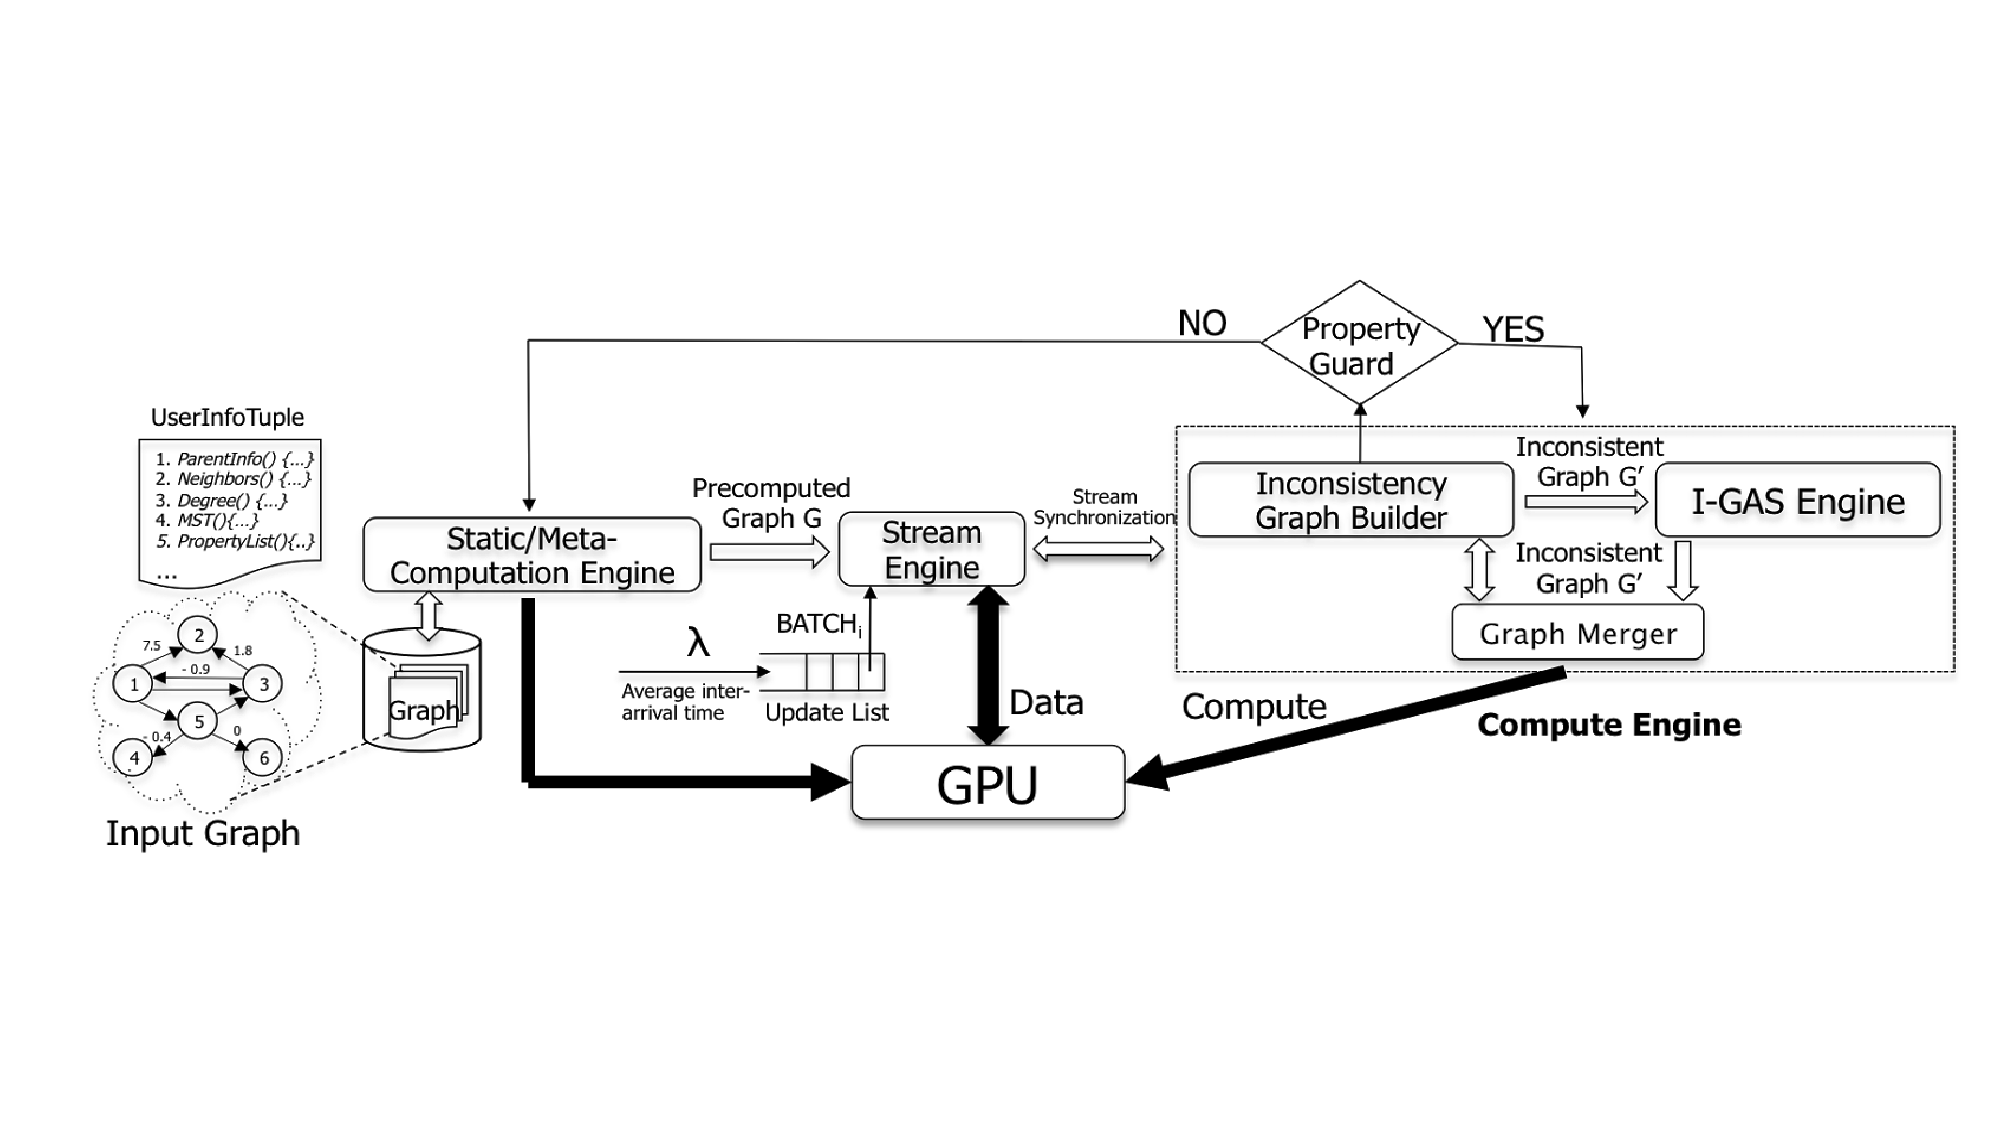
\includegraphics[width=1\columnwidth]{figures/framework.pdf}
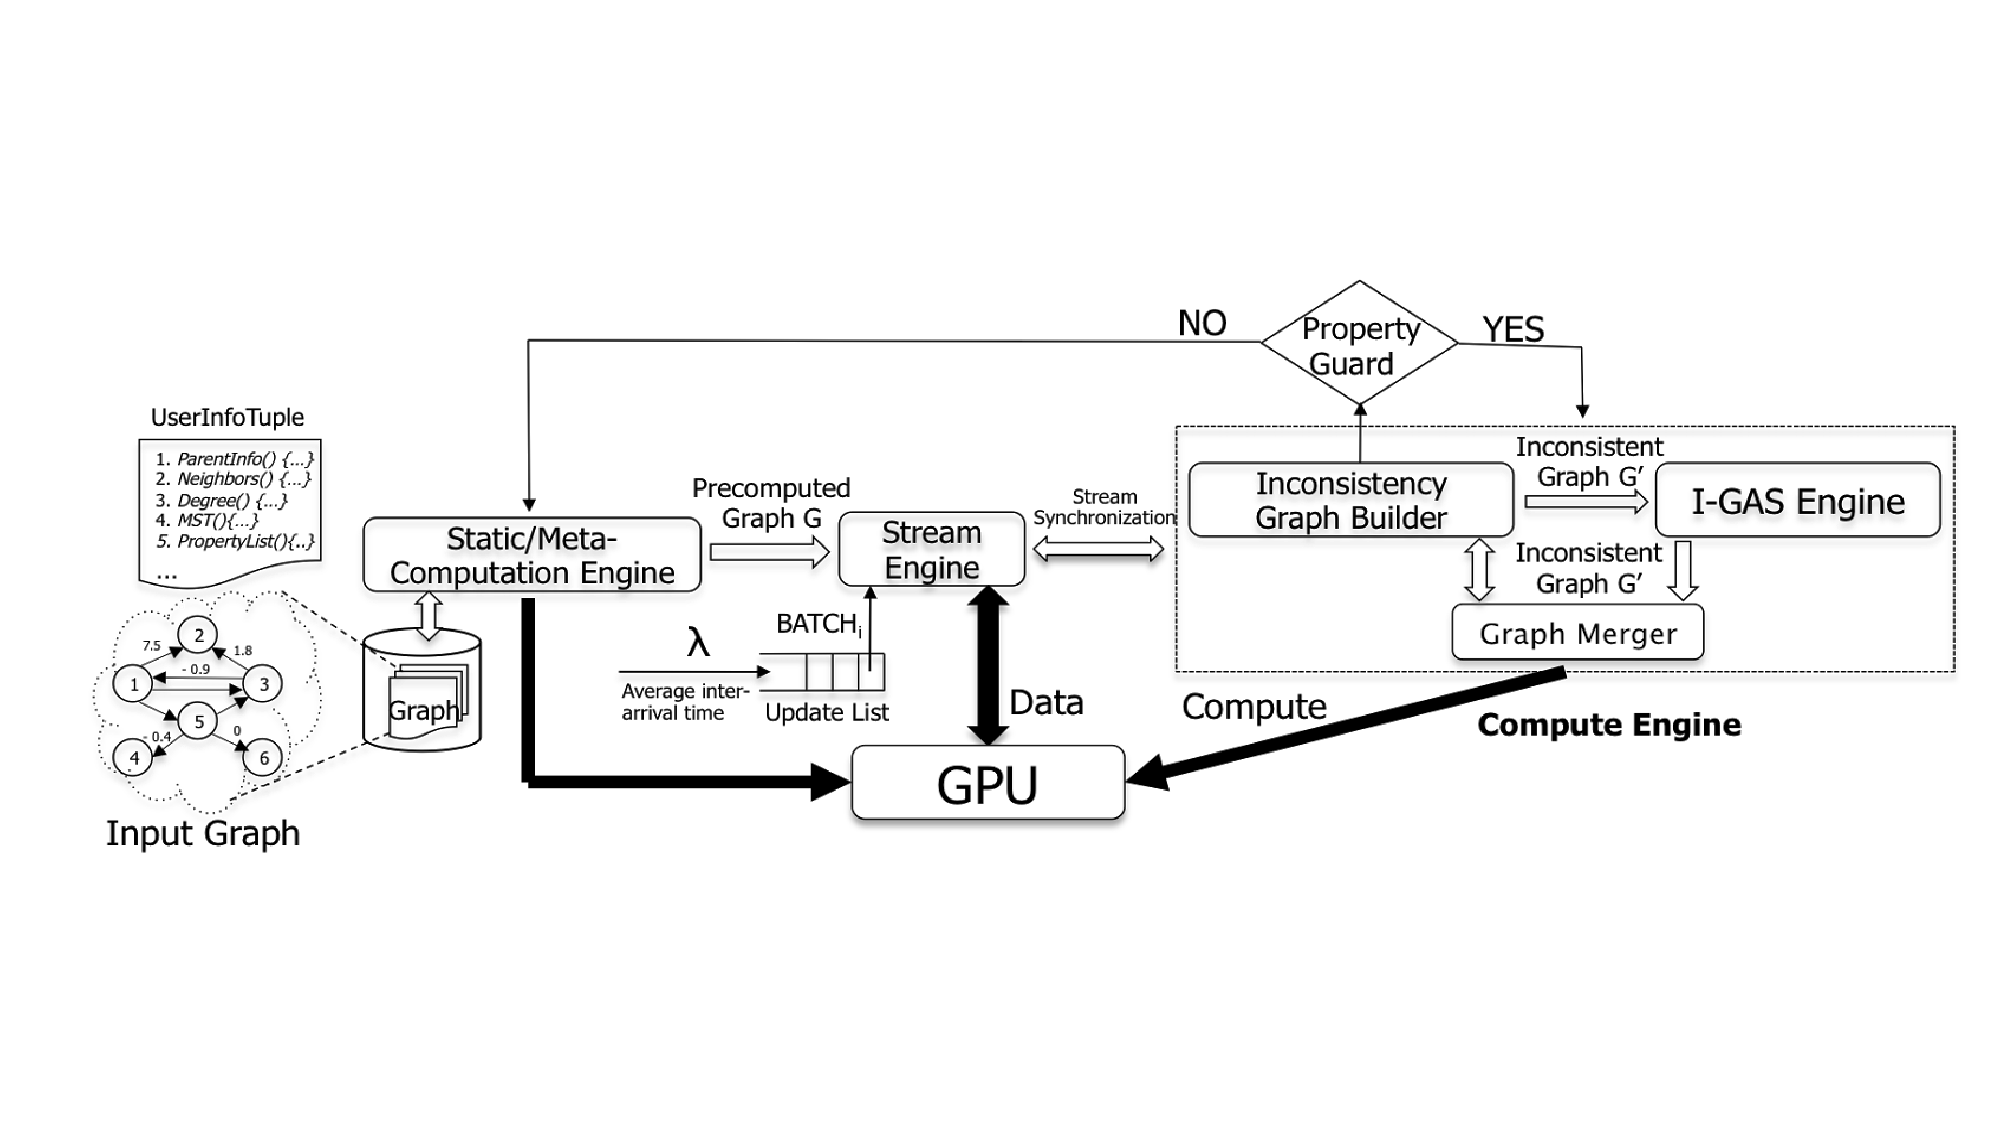
\includegraphics[width=\textwidth,height=\textheight,keepaspectratio]{figures/framework.pdf}
\caption{The software architecture diagram of EvoGraph.}
\label{fig:framework}
%\vspace{-0.5\baselineskip}
\end{figure}


%The EvoGraph framework can efficiently process evolving graphs that incrementally change over time due to edge or vertex insertions and/or deletions by seamlessly mapping the graph computation to leverage thousands of cores available on GPU.  The continuous stream of updates is divided into fixed size batches before being processed by EvoGraph in the order of their arrival. EvoGraph simplifies evolving graph analytics programming by supporting a multi-phase, asynchronous, dual path execution model described in detail in the following sections. Figure \ref{fig:framework} shows the general software architecture of EvoGraph which consists of six major components: Static-/Meta-computation Engine, Stream Engine, Inconsistency Graph Builder, I-GAS Engine and Graph Merger.  All of these components support GAS-based APIs. 
%
%\subsection{User Interface}
%Table \ref{tbl:table} shows the six user-defined functions for representing the different computation phases in EvoGraph. By customizing these functions, programmers can simply write sequential graph algorithms on the host CPU side. The runtime of EvoGraph will then generate parallelized code to incrementally process evolving graph updates and execute them on the targeted GPU. The user-defined functions include \textit{meta\_computation()}, \textit{build\_inconsistency\_list()}, \textit{CheckProperty()}, \textit{frontier\_activate()}, \textit{update\_inconsistency\_list()} and \textit{merge\_state()}, corresponding to the five computation phases of EvoGraph which are summarized as follows: 
%\begin{enumerate}
%  \item  \textbf{Static Graph and Metadata Preprocessing}: computing the GAS-based static version of the graph and any optional metadata that will be used later for incremental processing.
%  \item \textbf{Marking Out Graph Inconsistency}: creating a list of inconsistent vertices, and optionally, a user-defined subgraph G' whose states became inconsistent after applying a particular update batch.
%  \item \textbf{Determine the Execution Path Through Property Checking}: using the user-defined and built-in property list to examine the current update batch to proactively decide whether to run incremental processing or static recomputation.
% \item  \textbf{Incremental GAS (I-GAS)}: applying incremental version of the GAS programming model to move the computational frontier one step per iteration.
% \item   \textbf{State-Merging}: Merging the incremental and static graph states.
%\end{enumerate}
%
%
%\begin{figure}[!t]
%\centering
%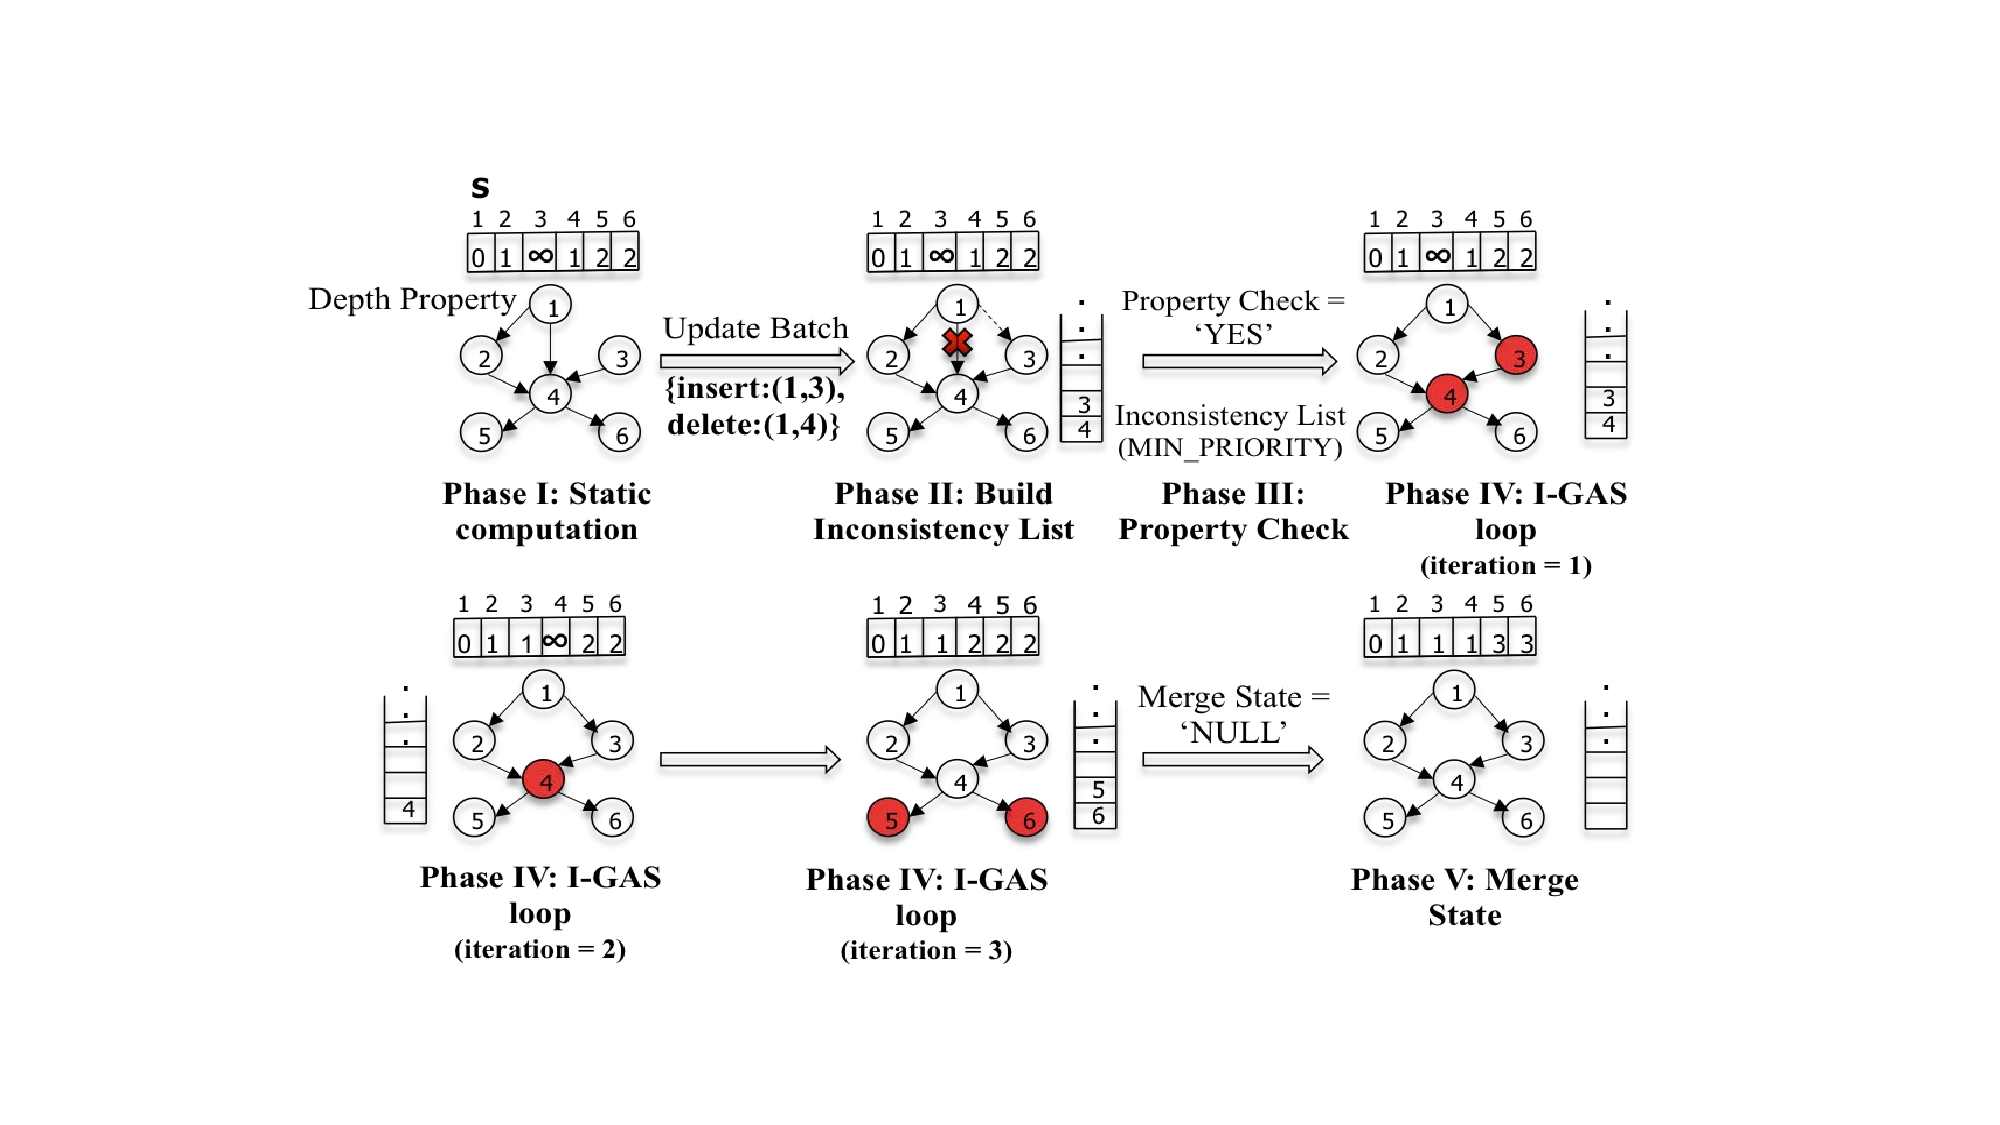
\includegraphics[width=1\columnwidth]{figures/bfs.pdf}
%\caption{Computation phases of an incremental BFS algorithm implemented in EvoGraph.}
%\label{fig:bfs}
%\vspace{-0.5\baselineskip}
%\end{figure}
%
%\begin{figure}[!t]
%\centering
%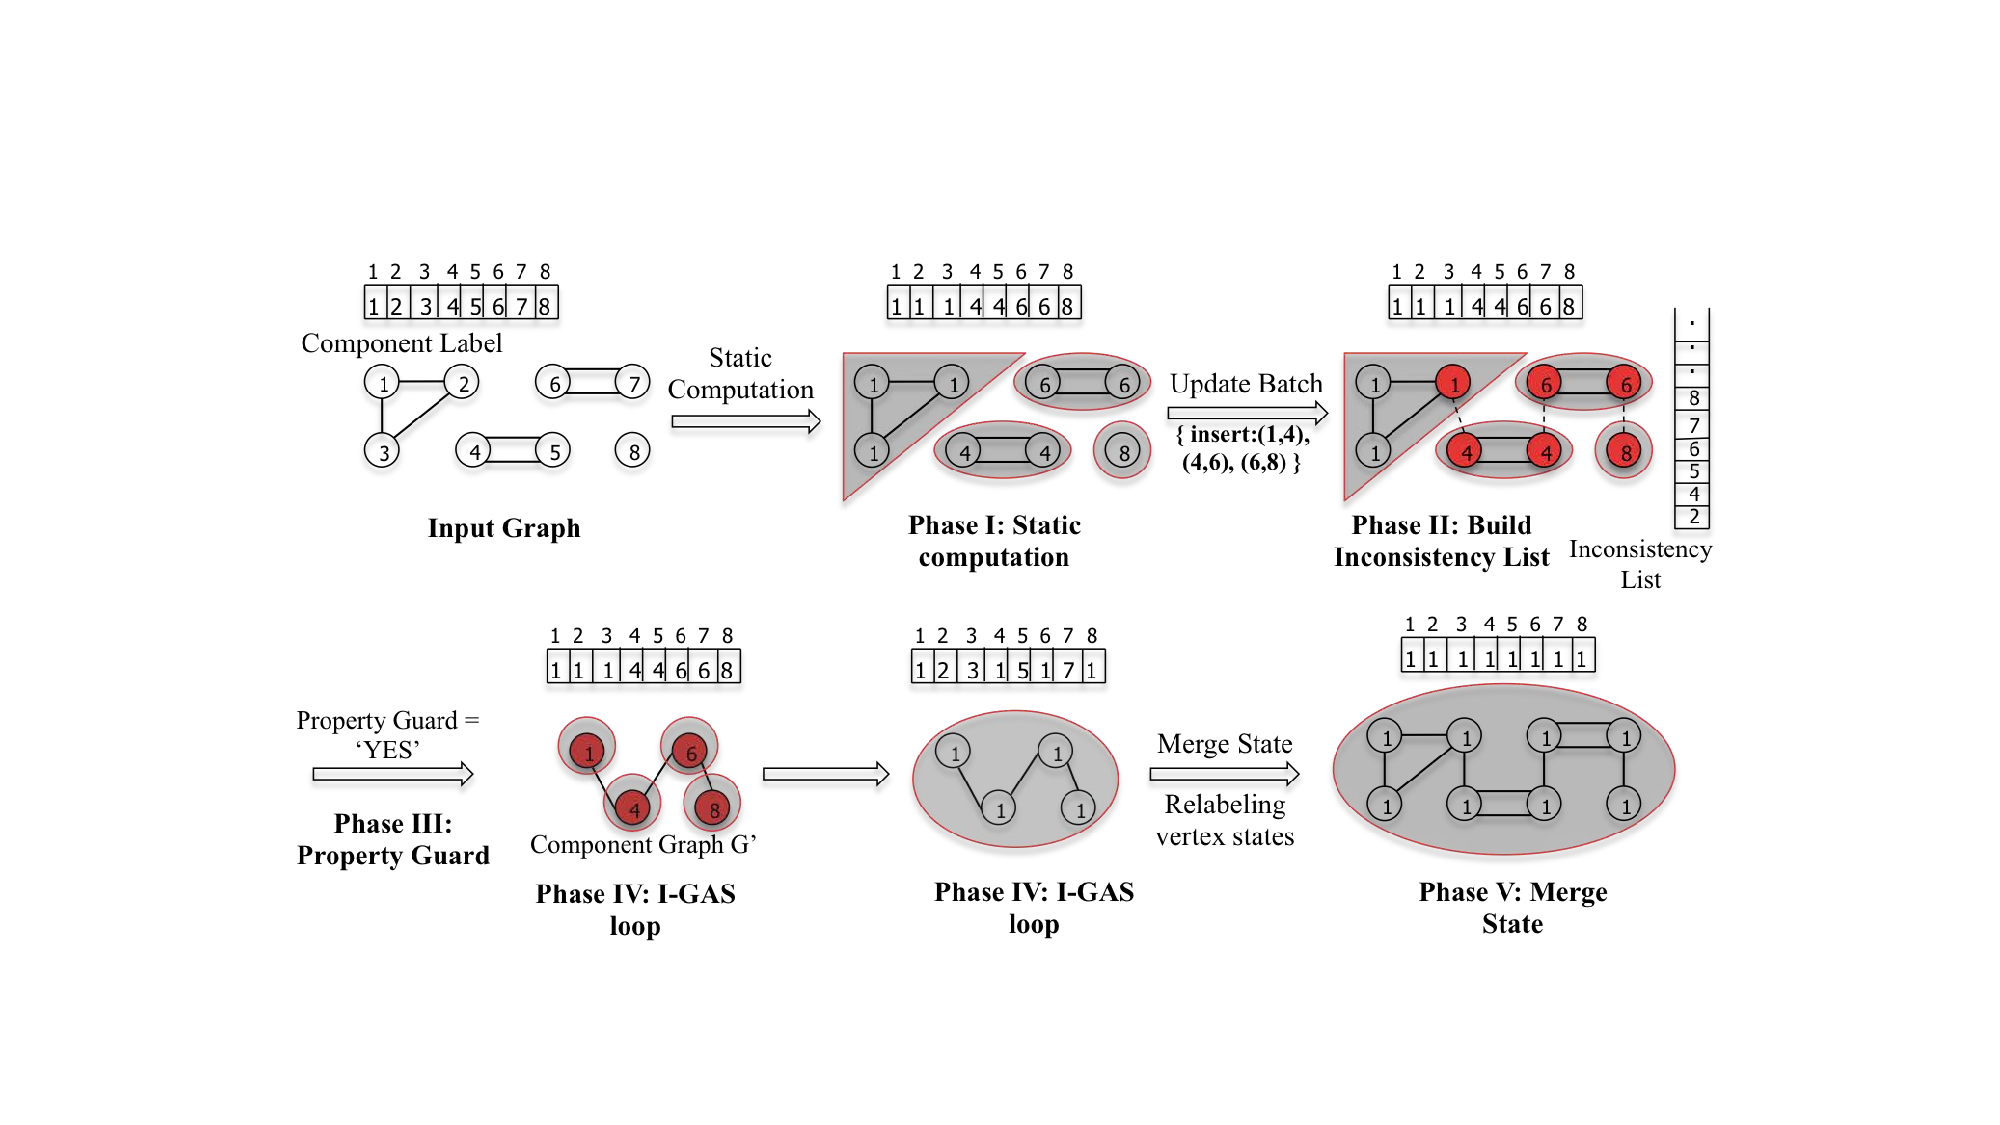
\includegraphics[width=1\columnwidth]{figures/cc.pdf}
%\caption{Computation phases of an incremental connected component (CC) algorithm implemented in EvoGraph.}
%\label{fig:cc}
%\vspace{-0.5\baselineskip}
%\end{figure}
%
%
%
%\begin{table*}[!t] 
%\caption{\textbf{Implementing Graph Algorithms in EvoGraph}} 
%\vspace{-0.3cm}
%\label{tbl:table} 
%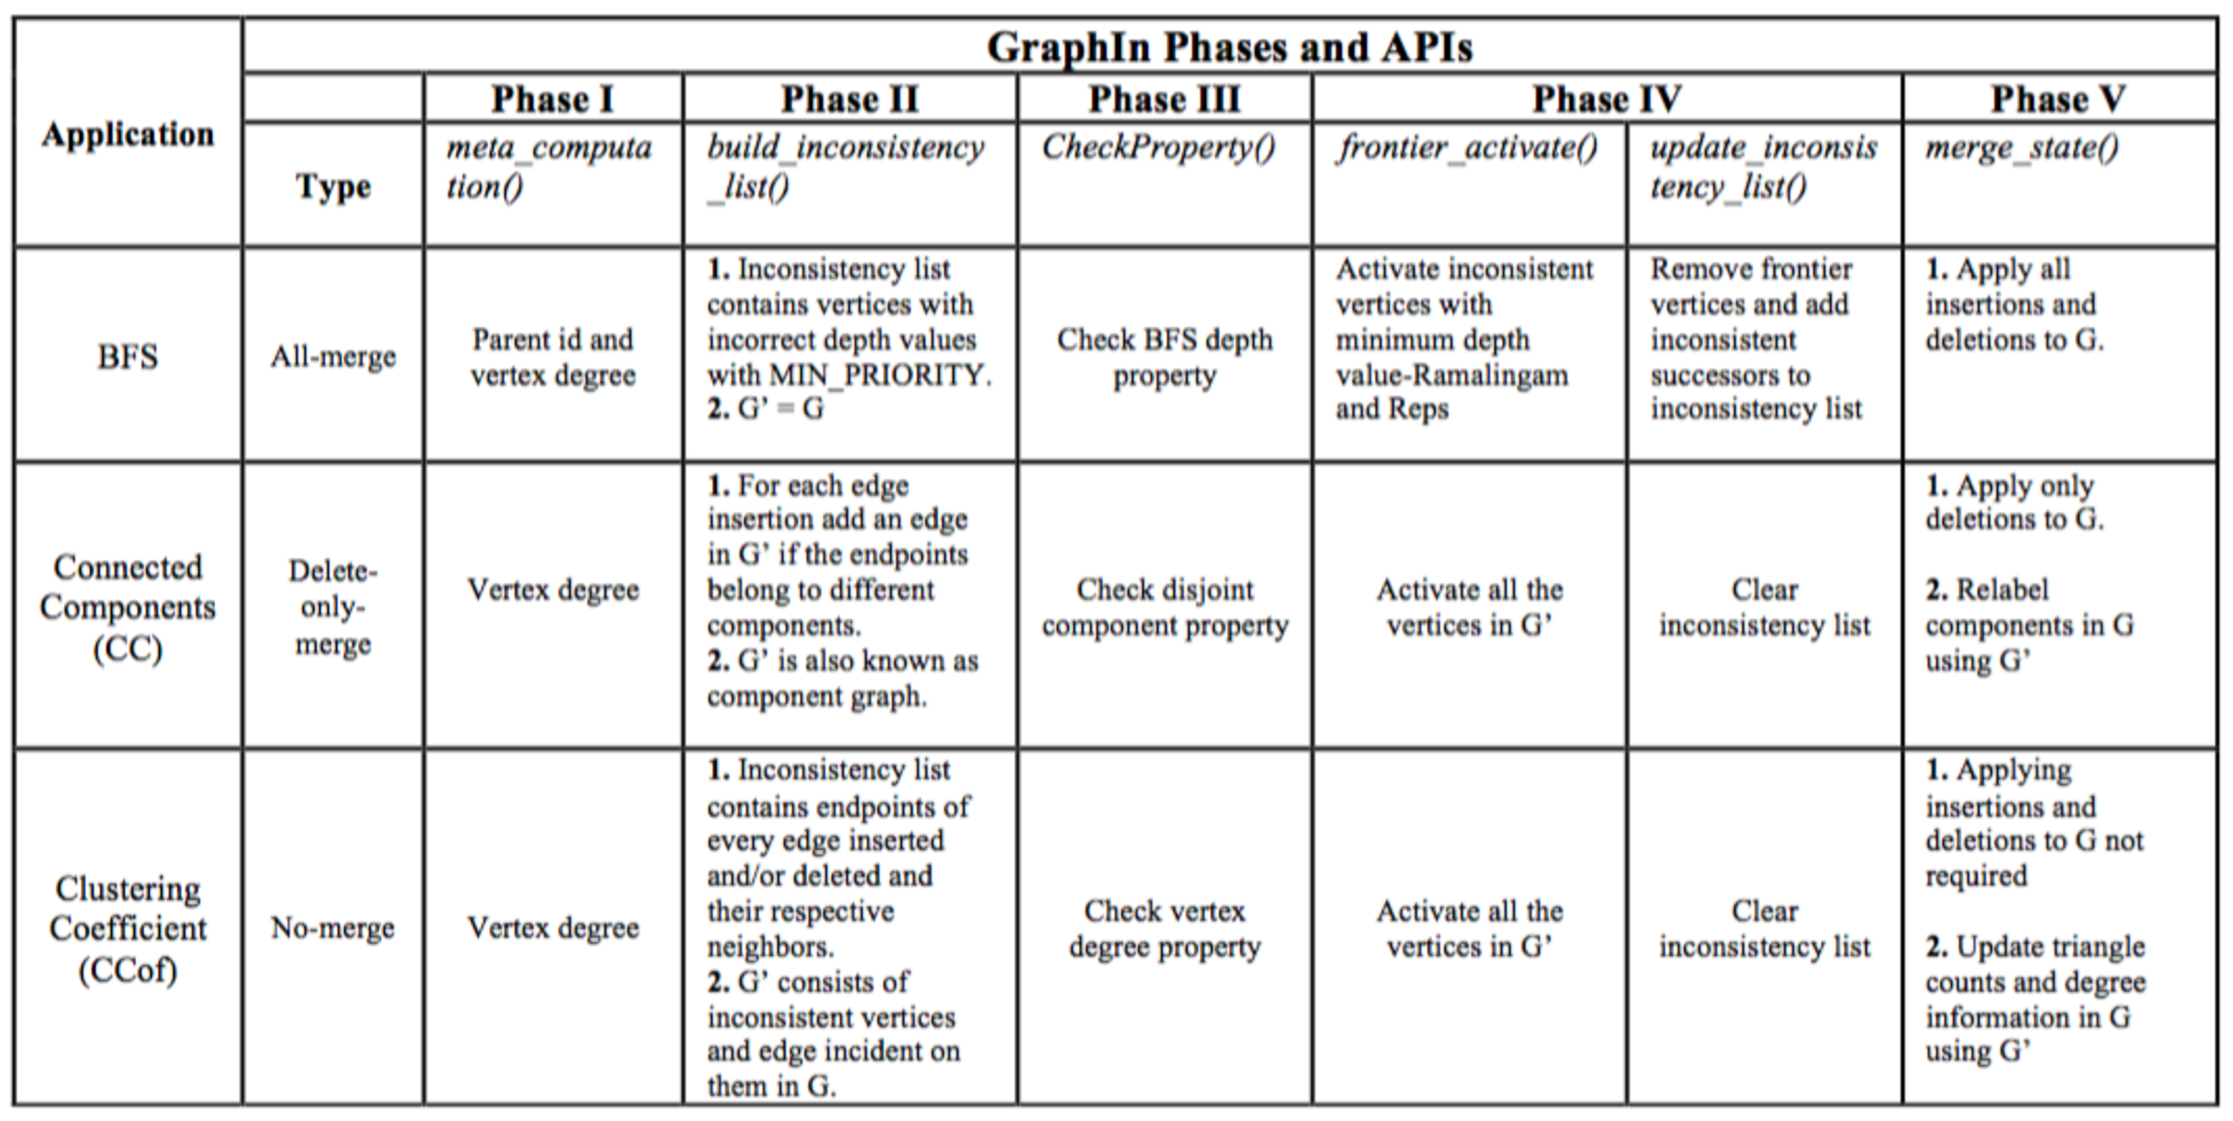
\includegraphics[width=\linewidth]{figures/table.pdf} 
%\vspace{-0.5cm}
%\end{table*}
%
%As an example, Figure \ref{fig:bfs} and \ref{fig:cc} illustrate the five computation phases in incremental Breath-First Search and Connected Component algorithms. Before discussing each of these phases in detail, we first look into the \textbf{Stream Engine} in Figure \ref{fig:framework}, which is in charge of optimizing data movement (between host and device) and context merging (discussed in Section 4.2.4). 

The EvoGraph framework can efficiently process evolving graphs that incrementally change over time due to edge or vertex insertions and/or deletions by seamlessly mapping the graph computation to leverage thousands of cores available on GPU.  The continuous stream of updates is divided into fixed size batches before being processed by EvoGraph in the order of their arrival. EvoGraph simplifies evolving graph analytics programming by supporting a multi-phase, asynchronous, property guarded execution model described in detail in the following sections. Figure \ref{fig:framework} shows the general software architecture of EvoGraph which consists of six major components: Static-/Meta-computation Engine, Stream Engine, Inconsistency Graph Builder, I-GAS Engine and Graph Merger.  All of these components support GAS-based APIs. 

\subsection{User Interface}
Table \ref{tbl:table} shows the six user-defined functions for representing the different computation phases in EvoGraph. By customizing these functions, programmers can simply write sequential graph algorithms on the host CPU side. The runtime of EvoGraph will then generate parallelized code to incrementally process evolving graph updates and execute them on the targeted GPU. The user-defined functions include \textit{meta\_computation()}, \textit{build\_inconsistency\_list()}, \textit{property\_guard()}, \textit{frontier\_activate()}, \textit{update\_inconsistency\_list()} and \textit{merge\_state()}, corresponding to the five computation phases of EvoGraph which are summarized as follows: 
\begin{enumerate}
  \item  \textbf{Static Graph and Metadata Preprocessing}: computing the static version of the graph and any optional metadata that will be used later for incremental processing.
  \item \textbf{Marking Out Graph Inconsistency}: creating a list of inconsistent vertices, and optionally, an inconsistent subgraph G'.
  \item \textbf{Determine the Execution Path by Property Checking}: using the user-defined and built-in property list to examine the current update batch to proactively decide between  incremental processing vs. static recomputation.
 \item  \textbf{Incremental GAS (I-GAS)}: applying incremental version of the GAS programming model to move the computational frontier one step per iteration.
 \item   \textbf{State-Merging}: Merging the incremental and static graph states.
\end{enumerate}


\begin{figure}[!t]
\centering
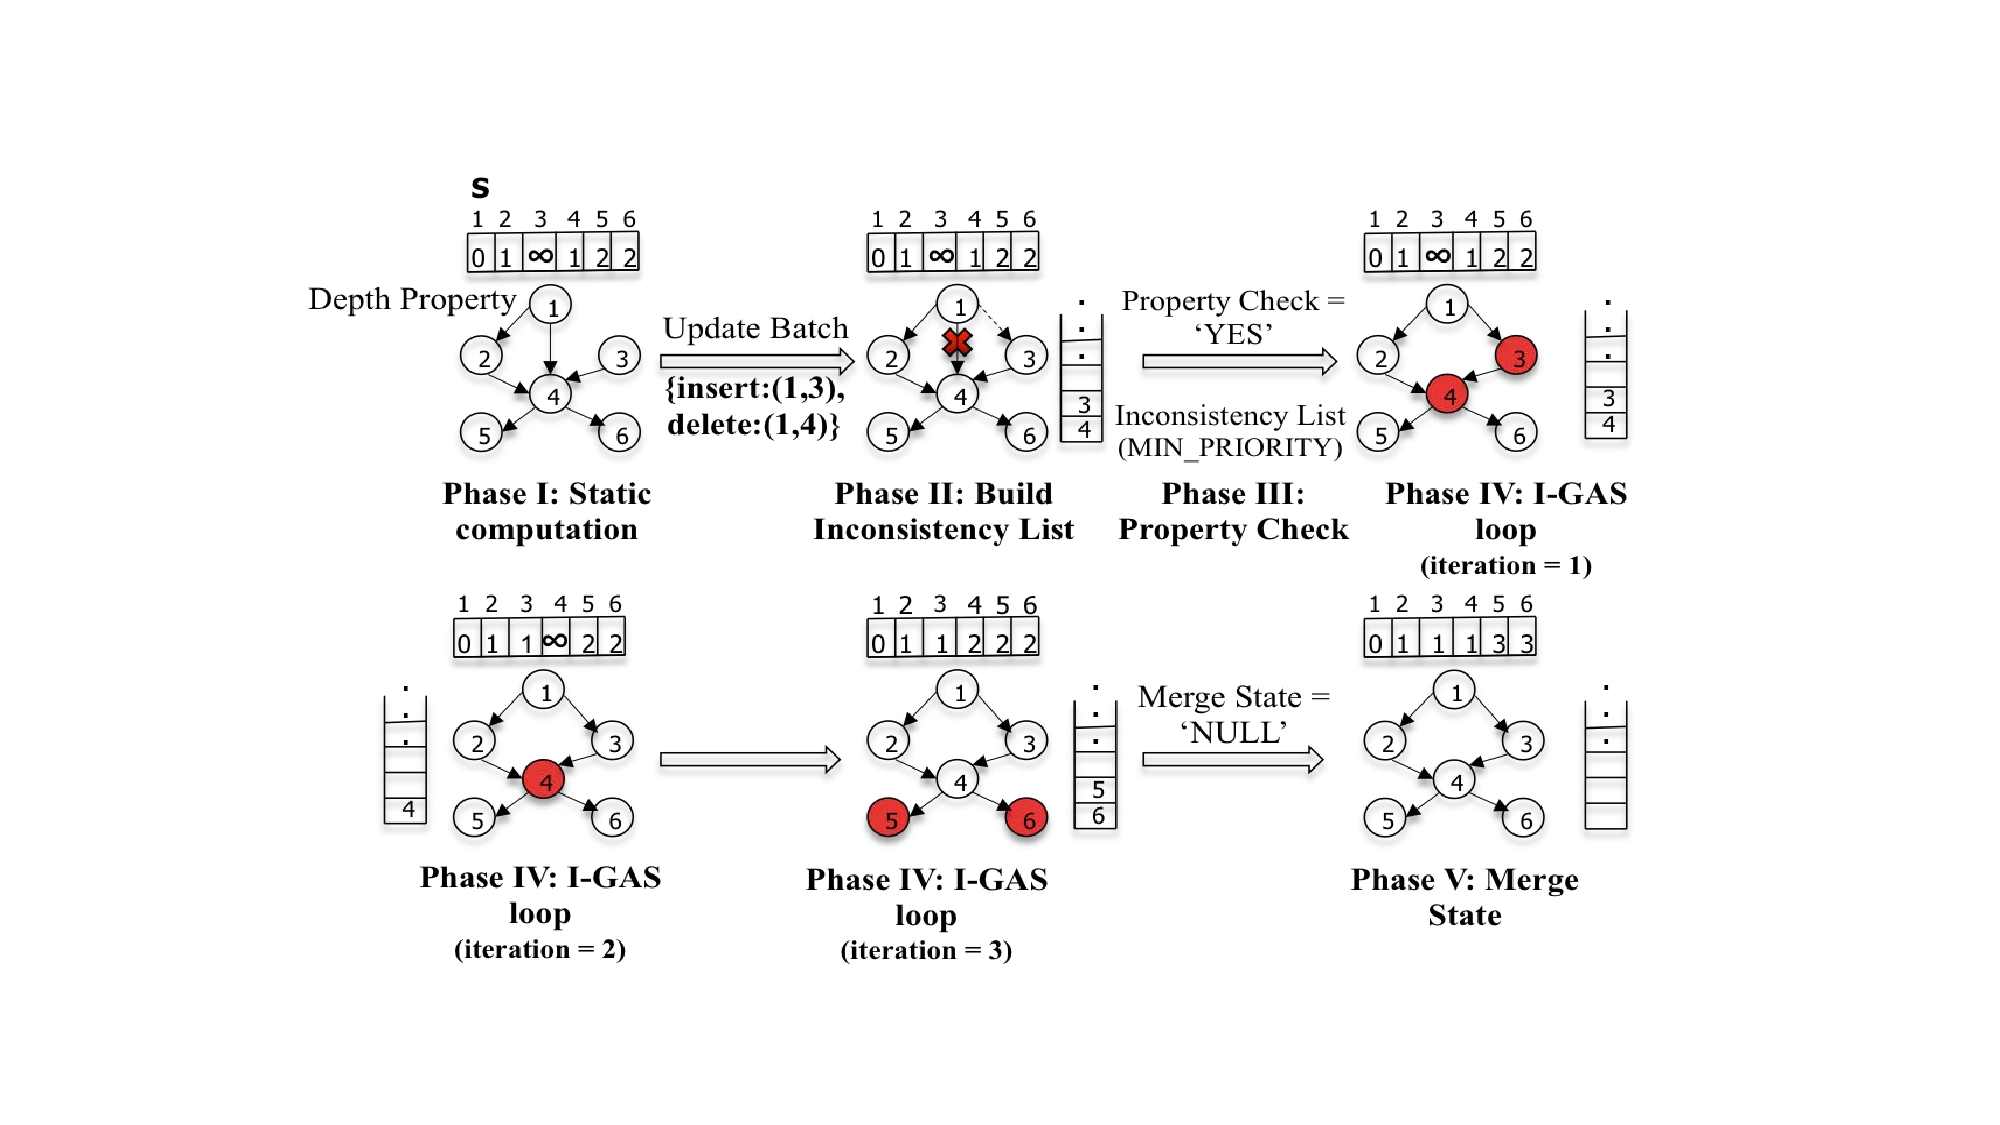
\includegraphics[width=1\columnwidth]{figures/bfs.pdf}
\caption{Computation phases of incremental BFS implemented in EvoGraph with inconsistent vertices marked red.}
\label{fig:bfs}
%\vspace{-0.5\baselineskip}
\end{figure}

\begin{figure}[!t]
\centering
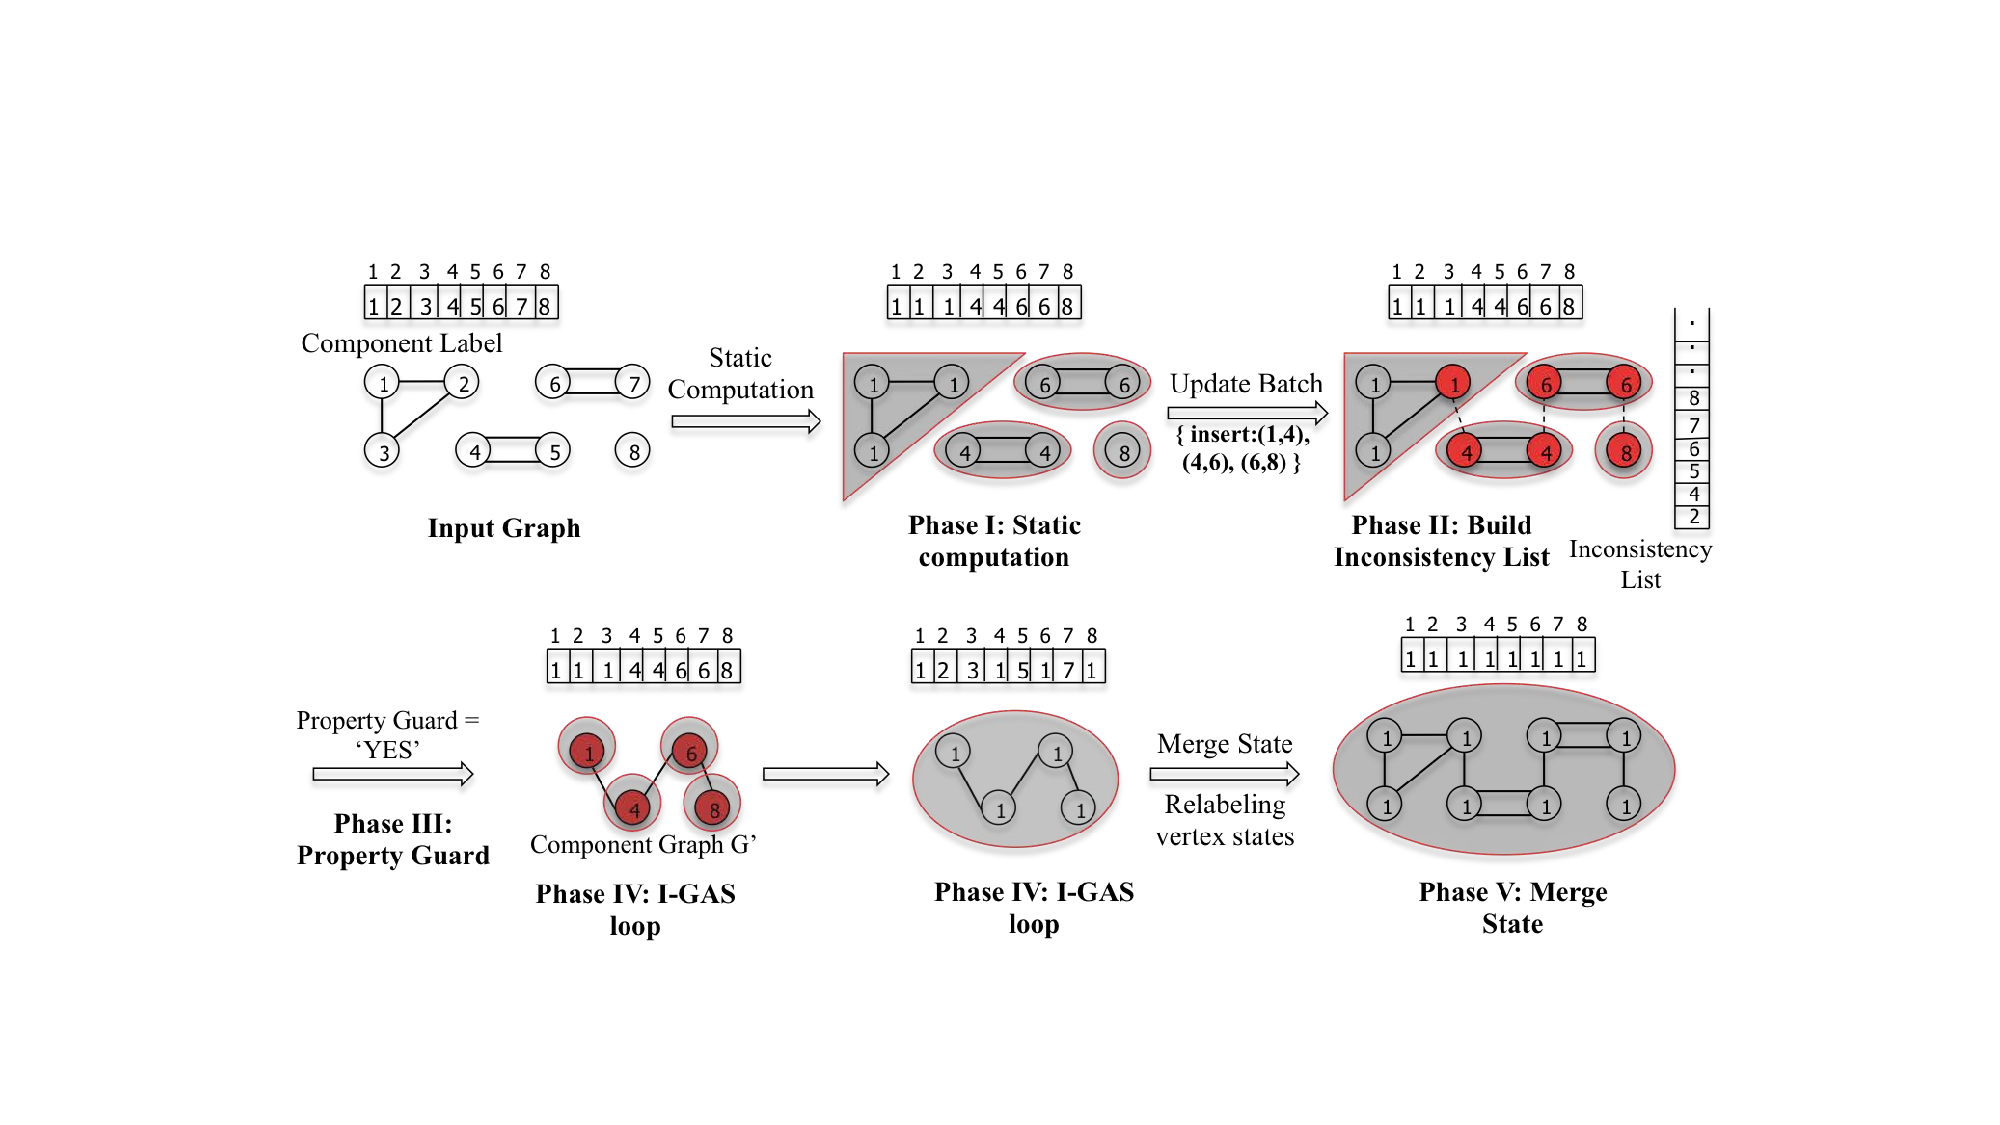
\includegraphics[width=1\columnwidth]{figures/cc.pdf}
\caption{Computation phases of incremental connected component (CC) implemented in EvoGraph with inconsistent vertices marked red.}
\label{fig:cc}
%\vspace{-0.5\baselineskip}
\end{figure}

\begin{table*}[!t] 
\caption{{Implementing Graph Algorithms in EvoGraph}} 
%\vspace{-0.2cm}
\label{tbl:table} 
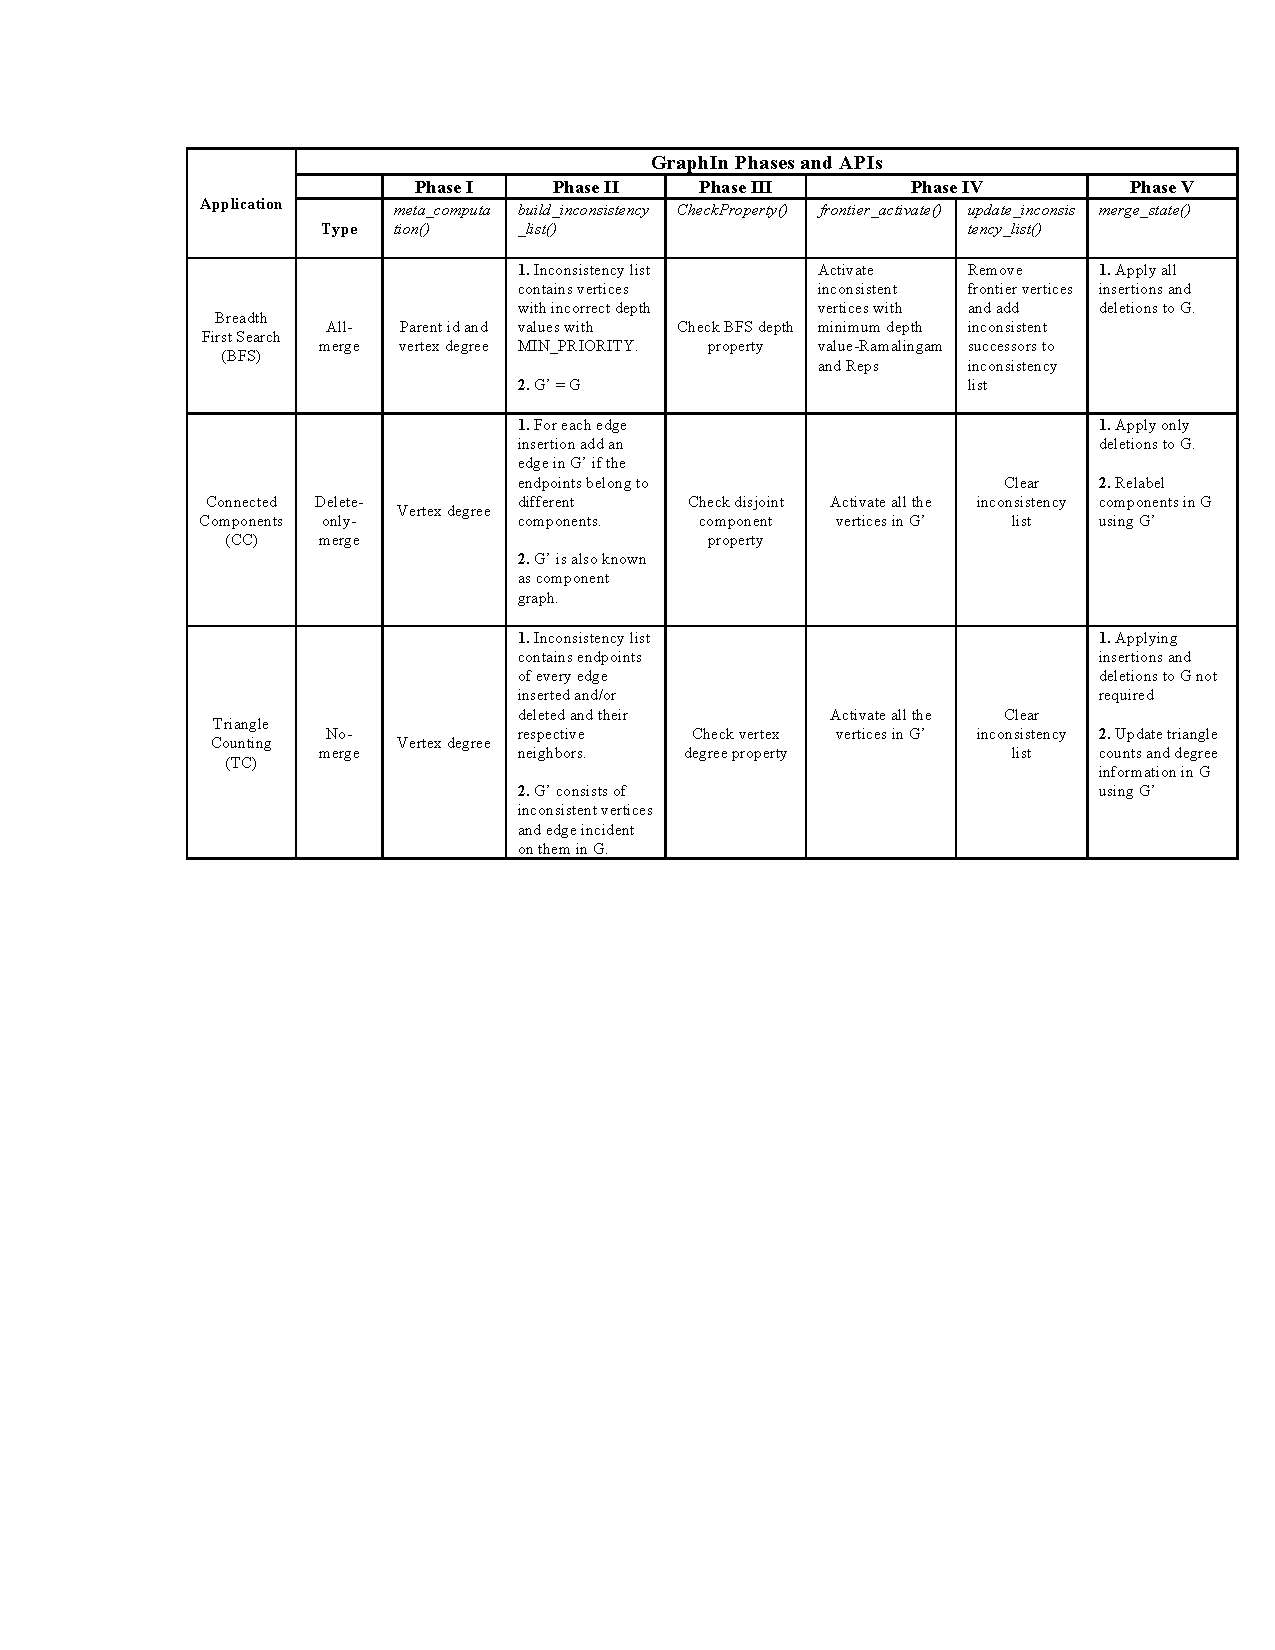
\includegraphics[width=\textwidth,height=\textheight,keepaspectratio]{figures/Big-Table.pdf}
%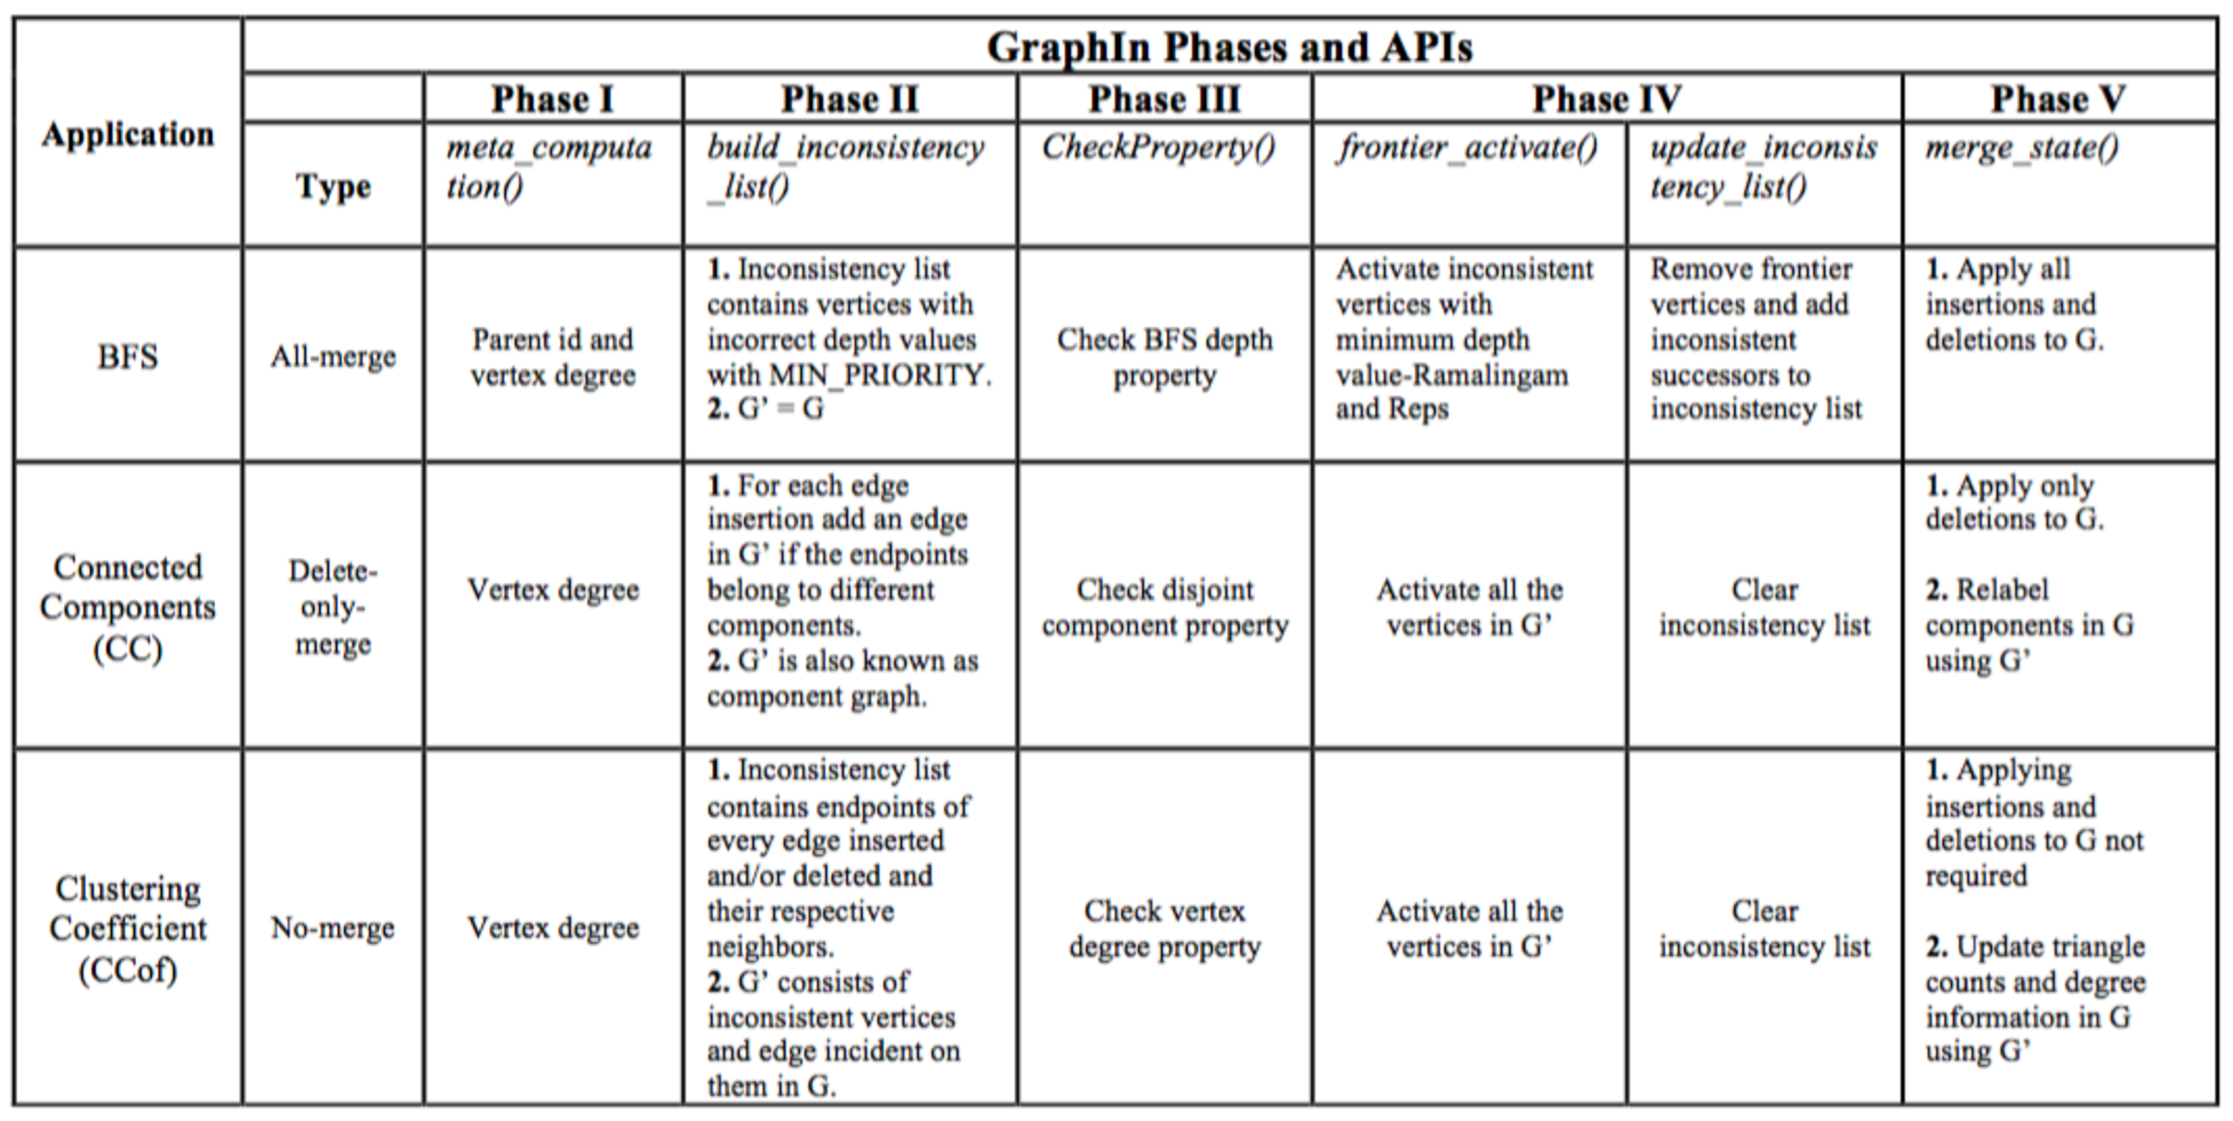
\includegraphics[width=\textwidth,height=\textheight,keepaspectratio]{figures/table.pdf}
%\vspace{-0.5cm} 
\end{table*}

As an example, Figure \ref{fig:bfs} and \ref{fig:cc} illustrate the five computation phases in incremental Breath-First Search (BFS) and Connected Component (CC) algorithms of which only CC requiring a separate inconsistent subgraph G' in Phase IV. Before discussing each of these phases in detail, we first look into the \textbf{Stream Engine} in Figure \ref{fig:framework}, which is in charge of optimizing data movement (between host and device) and context merging (discussed in Section 4.2.4). 

\subsection{Stream Engine: Data Movement and Context Merging}
%\textit{Stream Engine (SE)} is mainly responsible for two things: (i) efficient asynchronous data transfer between host and GPU, and (ii) context merging of static and incremental graph computation on the same GPU whenever required to enable multi-level GPU sharing. 

\begin{figure}[!t]
\centering
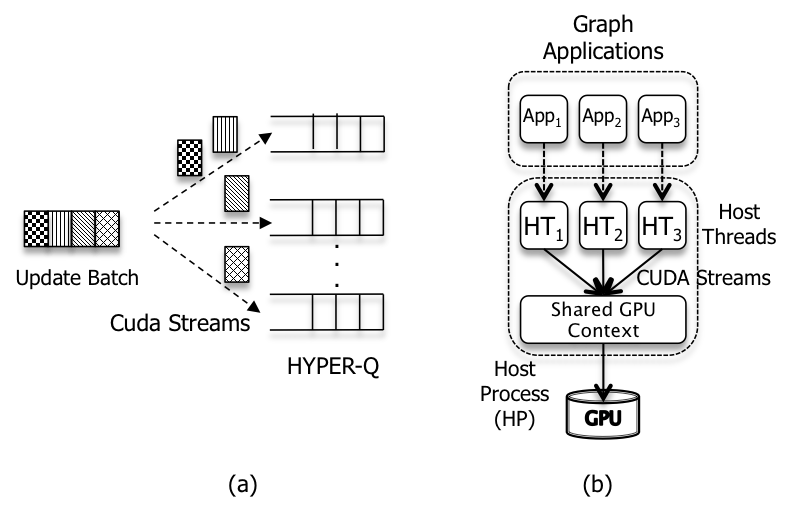
\includegraphics[width=\textwidth,height=\textheight,keepaspectratio]{figures/deep.png}
\caption{(a) Deep Copy mechanism in Stream Engine. (b) Context Merging Mechanism in Stream Engine.}
\label{fig:deep}
%\vspace{-1\baselineskip}
\end{figure}

%For (i), SE leverages CUDA Streams, double buffering, and hardware support like \textit{Hyper-Qs} provided by the architectures such as NVIDIA Kepler and Maxwell, to effectively overlap data streaming and computation. As shown in Figure \ref{fig:deep}(a), SE spawns separate CUDA Streams to launch multiple kernels simultaneously and transfer batched of incremental updates to the graph asynchronously, overlapping memory copies within and across computation phases. Furthermore, EvoGraph uses separate CUDA Streams to enable deep copy operations [ ] in order to take advantage of the large number of hardware queues offered by modern GPU architectures. This is motivated by the fact that an update batch in EvoGraph is not a single contiguous byte-array, but consists of many sub-arrays that contain edge, vertex, and vertex/edge property update information. EvoGraph exploits this important feature by not moving the entire update batch in one copy performed by a single CUDA stream, but instead making SE to dynamically spawn multiple CUDA Streams to move these sub-arrays to GPU. The outcome is the concurrent usage of the GPU's many hardware queues, which consequently improves the overall throughput. 
%
%As shown in Figure \ref{fig:deep}(a), SE achieves (ii) by packing multiple applications' GPU contexts into a single protection domain on-the-fly to maximize GPU resource utilization and avoid core idling. When the first GPU request from an graph application (static or incremental computation) arrives, SE creates a separate CUDA stream object for it by calling \textit{cudaStreamCreate()}, the handler to which is stored in a thread local storage. Using this handler, subsequent requests from this graph application will be dispatched over this designated stream. Upon application exit or \textit{cudaThreadExit()}, SE tears down the stream by calling \textit{cudaStreamDestroy()} on the stream handler. Additionally, the GPU operations that synchronize the application and the device are replaced with their CUDA stream counterparts, e.g., \textit{cudaDeviceSynchronize()} is replaced with \textit{cudaStreamSynchronize()}. This ensures that all the applications packed into a single GPU context associated with a particular GPU are not blocked when one of them explicitly synchronizes its host thread with the device. Next we discuss each computation phase in detail. 


The \textit{Stream Engine (SE)} is mainly responsible for: (i) efficient asynchronous data transfer between host and GPU, and (ii) context merging of static and incremental computation on the same GPU to enable multi-level GPU sharing. 

For (i), SE leverages CUDA Streams, double buffering, and hardware support like \textit{Hyper-Qs} provided by the architectures such as NVIDIA Kepler and Maxwell, to effectively overlap data streaming and computation. SE spawns separate CUDA Streams to launch multiple kernels simultaneously and transfer batches of incremental updates to the graph asynchronously, overlapping memory copies within and across computation phases. Furthermore, as shown in Figure \ref{fig:deep}(a), EvoGraph uses separate CUDA Streams to enable deep copy operations~\cite{cuda7},~\cite{GraphReduce} in order to take advantage of the large number of hardware queues offered by modern GPU architectures. This is motivated by the fact that an update batch in EvoGraph is not a single contiguous byte-array, but consists of many sub-arrays that contain edge, vertex, and vertex/edge property update information. EvoGraph exploits this by not moving the entire update batch in one copy performed by a single CUDA stream, but instead making SE to dynamically spawn multiple CUDA Streams to move these sub-arrays to GPU. The outcome is the concurrent usage of the GPU's many hardware queues, which consequently improves the overall throughput. 

As shown in Figure \ref{fig:deep}(b), SE achieves (ii) by packing multiple applications' GPU contexts into a single protection domain on-the-fly to maximize GPU resource utilization and avoid core idling. When a GPU request from a graph application (static or incremental computation) arrives, SE creates a separate CUDA stream object for it by calling \textit{cudaStreamCreate()}, the handler to which is stored in a thread local storage. Using this handler, subsequent requests from this application is dispatched over this designated stream. Upon application exit, SE tears down the stream by calling \textit{cudaStreamDestroy()} on the stream handler. Additionally, the GPU operations that synchronize the application and the device are replaced with their CUDA stream counterparts, e.g., \textit{cudaDeviceSynchronize()} is replaced with \textit{cudaStreamSynchronize()}. This ensures that all the applications packed into a single GPU context associated with a particular GPU are not blocked when one of them explicitly synchronizes its host thread with the device. Next we discuss each computation phase in detail. 



\subsection{Computation Phases in EvoGraph}

%\textbf{Phase I: Static Graph and Metadata Preprocessing}. As shown in Figure \ref{fig:bfs} and Table \ref{tbl:table}, this phase has two main purposes. First, it computes the static version of the input graph based on the traditional GAS model (Section 4.1.1). Theoretically speaking, any GAS-based static graph processing frameworks can be applied here for the static computation. In this work, we chose the highly efficient GPU static-graph processing framework GraphReduce as part for our static computation engine. Second, it computes the graph property metadata, including parent id, vertex degree, neighbors, and minimum spanning tree (MST). These property metadata play an important role in processing incremental graph algorithm in the upcoming phases. For instance, Table \ref{tbl:table} lists what metadata are required to be computed in Phase I for different incremental graph algorithms.  
%
%
%
%% This phase is responsible for computing (1) the static version of the graph using the traditional GAS programming model, and (2) metadata that will be needed in the incremental logic. Since the static graph computation follows the GAS model, any graph processing framework that supports GAS can theoretically be used as a Static-Computation Engine. In this work, we chose the state-of-the-art GPU static-graph processing framework GraphReduce as the core for our static graph computation. Metadata computation (\textit{meta\_computation()}) involves the computation of static graph properties such as parents, neighbors, vertex degree, and minimum spanning tree (MST). It will be needed by certain incremental algorithm in the later phases. For example, shown in Figure \ref{fig:bfs}, incremental BFS requires parent information during Phase IV.
%
%\textbf{Phase II: Marking Out Graph Inconsistency}. As illustrated in Figure \ref{fig:bfs} and \ref{fig:cc}, this is the phase where incremental graph processing begins. This phase identifies the inconsistent part of the graph after the batch update through the \textit{build\_inconsistency\_list()} function shown in Table \ref{tbl:table}. This function is user-defined and it takes the update batch information (e.g., edge/vertex insertions and/or deletions) and the priority attribute for each vertex to build a list of inconsistent vertices. EvoGraph also provides an option for users to construct a sub-graph G' to describe the inconsistency which can be used later. Table \ref{tbl:table} lists the action items from Phase II for different graph algorithms.  
%
%\textbf{Phase III: Determine the Execution Path Through Property Checking}. This is the phase that decides which execution path, incremental processing or static recomputation, should be taken based on the area effect caused by the incremental graph algorithms. More specifically, if an incremental algorithm causes the majority portion of the graph to become inconsistent, incremental processing may not be a better option than static recomputation due to its extra execution overheads. For example, show in Figure \ref{fig:bfs}, if an incremental update affects a large number of vertices close to the root of the BFS tree, it is more efficient to just execute with static recomputation. For every update batch, EvoGraph uses a selected set of graph properties (e.g., degree, neighbor info, distance, depth, etc) that will affect the runtime performance of the algorithm to make the selection for execution path.  Table \ref{tbl:table} shows such essential graph properties for different graph algorithms, and the corresponding API call \textit{property\_guard()}. Using BFS as an example, for each batch update, EvoGraph will check the vertex depth threshold below which incremental processing will degrade the performance, and the inconsistency fraction which is the percentage of inconsistent vertices that are under the vertex depth. For instance, EvoGraph with input $X$ will stop benefit from incremental processing if more than 80\% (inconsistency fraction) of the inconsistent vertices have vertex depth less than 3. We want to emphasize that these selected graph properties are input and algorithm dependent and can be tuned for max performance by users. 
%
%
%
%%As discussed in Section 4.2.3, there are classes of incremental algorithms that cause large portions of the graph to become inconsistent and hence can result in recomputation over the entire graph. For these classes, incremental processing will not achieve any performance benefit over static recomputation and may even result in performance degradation due to the overheads associated with the incremental execution. To address this, EvoGraph allows users to define a heuristic for determining which one of the two computation (incremental processing or static recomputation) should be applied. Users may select from a set of predefined graph properties (e.g., degree, neighbor info, distance, depth, etc) or define their own properties that they believe will affect the runtime of the targeted incremental algorithm. EvoGraph will then use the selected properties to decide whether to run incremental or static recomputation by calling the \textit{property\_check()} API for each update batch. We name this \textit{property-based dual path execution}. \textit{property\_check()} takes four parameters: inconsistency\_list, property\_list, threshold\_vector, and threshold\_fraction. Property List defines the set of graph properties under consideration. Threshold Vector defines a set of thresholds for properties in the Property List, above (or below) which the performance of incremental processing will drastically degrade. Finally, Threshold Fraction defines the fraction of inconsistent vertices that are above (or below) the corresponding property threshold. 
%%
%%Using Figure \ref{fig:bfs} as an example, when running incremental BFS, the vertex depth is one of the properties defined in the property list, with the property threshold of 2 and the threshold fraction of 0.3.  In this case, EvoGraph would switch to static BFS recomputation if $>$ 30\% of inconsistent vertices have BFS depth $<$ 2. This is in line with the observation that if an update affects a large number of vertices closer to the root of BFS tree, it is better to run a full static recomputation. Note that the thresholds for these properties and the fraction of inconsistent vertices are user-tunable parameters that are algorithm and dataset dependent and require training to derive their optimal values.
%
%
%
%%\textbf{Phase IV: Incremental GAS}. Incremental GAS or I-GAS phase ensures that only the inconsistent or affected portion of the graph is recomputed incrementally, not the entire graph. The I-GAS Engine shown in Figure \ref{fig:framework} identifies the overlap between two consecutive versions of the evolving graph and incrementally processes the graph by only operating on the new computational frontier. With the new I-GAS computation model, users can implement the I-GAS programs as well as the \textit{frontier\_activate()} and update\_inconsistency\_list() APIs. Listing \ref{lst:igas} shows a typical I-GAS loop, which is comprised of  three basic steps that are iterated over until the inconsistency list becomes empty. It starts with a set of inconsistent vertices and calls frontier\_activate() to activate the next computational frontier using the vertex priority defined in \textit{Phase II}, and then runs an I-GAS program. An I-GAS program consists of incremental versions of the Gather, Apply and Scatter functions. By default, an I-GAS program is the same as an GAS program for static execution, but users can modify it for incremental processing. Finally, the new computational frontier information is used to update the vertex inconsistency list. Figure \ref{fig:bfs} details this phase with an example. 
%
%
%\textbf{Phase IV: Incremental GAS}. As discussed in Section 4.2.1, we propose Incremental GAS or I-GAS in this work to compute the vertex states only for those inconsistent vertices that are affected by the batch updates, while maintaining the vertex states for the rest to significantly reduce the overall execution time. More specifically, I-GAS will only incrementally operate on the new computational frontiers \footnote{Computational frontier or frontier size describes the number of active vertices or edges in a given iteration of a graph algorithm.} without processing the overlap between two consecutive versions of the graph. Figure \ref{fig:bfs} and \ref{fig:cc} show two comprehensive examples of I-GAS loops for BFS and CC. Listing \ref{lst:igas} shows the typical I-GAS computation loop per update batch. Basically, EvoGraph maintains a inconsistency list and the three functions will iterate until the list becomes empty. Note that in each iteration function \textit{frontier\_activate()} will activate new computational frontiers using the vertex priority to feed \text{IGAS()}, which calls incremental versions of Gather, Apply and Scatter. Finally, the new frontier information will update the inconsistency list.


\textbf{Phase I: Static Graph and Metadata Preprocessing}. As shown in Figure \ref{fig:bfs} and Table \ref{tbl:table}, this phase has two main purposes. First, it computes the static version of the input graph based on the traditional GAS model (Section 4.1.1). Theoretically speaking, any GAS-based static graph processing frameworks can be applied here for the static computation. In this work, we chose the highly efficient GPU-based static-graph processing framework GraphReduce as our static computation engine. Second, it computes the graph property metadata, such as parent id, vertex degree, neighbors, minimum spanning tree (MST). These property metadata play an important role in processing incremental graph algorithm in the upcoming phases. For instance, Table \ref{tbl:table} lists what metadata are required to be computed in Phase I for different incremental graph algorithms.  



% This phase is responsible for computing (1) the static version of the graph using the traditional GAS programming model, and (2) metadata that will be needed in the incremental logic. Since the static graph computation follows the GAS model, any graph processing framework that supports GAS can theoretically be used as a Static-Computation Engine. In this work, we chose the state-of-the-art GPU static-graph processing framework GraphReduce as the core for our static graph computation. Metadata computation (\textit{meta\_computation()}) involves the computation of static graph properties such as parents, neighbors, vertex degree, and minimum spanning tree (MST). It will be needed by certain incremental algorithm in the later phases. For example, shown in Figure \ref{fig:bfs}, incremental BFS requires parent information during Phase IV.

\textbf{Phase II: Marking Out Graph Inconsistency}. As illustrated in Figure \ref{fig:bfs} and \ref{fig:cc}, this is the phase where incremental graph processing begins. This phase identifies the inconsistent part of the graph, after applying the update batch, using the \textit{build\_inconsistency\_list()} function shown in Table \ref{tbl:table}. This user-defined function takes the update batch information (e.g., edge/vertex insertions and/or deletions) and the priority attribute for each vertex to build a list of inconsistent vertices. EvoGraph also provides an option for users to construct an inconsistent sub-graph G' which can be used later. Table \ref{tbl:table} lists the action items from Phase II for different graph algorithms.  

\textbf{Phase III: Determine the Execution Path Through Property Checking}. %This is the phase that decides which execution path, incremental processing or static recomputation, should be taken based on the area effect caused by the incremental graph algorithms. More specifically, if an incremental algorithm causes the majority portion of the graph to become inconsistent, incremental processing may not be a better option than static recomputation due to its extra execution overheads. For example, if an incremental update affects a large number of vertices close to the root of the BFS tree, it is more efficient to just execute with static recomputation. For every update batch, EvoGraph uses a selected set of graph properties (e.g., degree, neighbor info, distance, depth, etc) that will affect the runtime performance of the algorithm to make the selection for execution path.  Table \ref{tbl:table} shows such essential graph properties for different graph algorithms, and the corresponding API call \textit{property\_guard()}. Using BFS as an example, for each batch update, EvoGraph will check the vertex depth threshold below which incremental processing will degrade the performance, and the inconsistency fraction which is the percentage of inconsistent vertices that are under the vertex depth. For instance, EvoGraph with batch $X$ will stop benefiting from incremental processing if more than 80\% (inconsistency fraction) of the inconsistent vertices have vertex depth less than 3. We want to emphasize that these selected graph properties are input and algorithm dependent and can be tuned for optimal performance by users. 



As discussed in Section 4.2.3, there are classes of incremental algorithms that cause large portions of the graph to become inconsistent and hence can result in recomputation over the entire graph. For these classes, incremental processing will not achieve any performance benefit over static recomputation and may even result in performance degradation due to the overheads associated with the incremental execution. To address this, EvoGraph allows users to define a heuristic for determining which one of the two computation (incremental processing or static recomputation) should be applied. Users may select from a set of predefined graph properties (e.g., degree, neighbor info, distance, depth, etc) or define their own properties that they believe will affect the runtime of the targeted incremental algorithm. EvoGraph will then use the selected properties to decide whether to run incremental or static recomputation by calling the \textit{property\_guard()} API for each update batch. We name this \textit{property-based dual path execution}. \textit{property\_guard()} takes four parameters: inconsistency\_list, property\_list, threshold\_vector, and threshold\_fraction. Property List defines the set of graph properties under consideration. Threshold Vector defines a set of thresholds for properties in the Property List, above (or below) which the performance of incremental processing will drastically degrade. Finally, Threshold Fraction defines the fraction of inconsistent vertices that are above (or below) the corresponding property threshold. 

Using Figure \ref{fig:bfs} as an example, when running incremental BFS, the vertex depth is one of the properties defined in the property list, with the property threshold of 2 and the threshold fraction of 0.3.  In this case, EvoGraph would switch to static BFS recomputation if $>$ 30\% of inconsistent vertices have BFS depth $<$ 2. This is in line with the observation that if an update affects a large number of vertices closer to the root of BFS tree, it is better to run a full static recomputation. Note that the thresholds for these properties and the fraction of inconsistent vertices are user-tunable parameters that are algorithm and dataset dependent and require training to derive their optimal values.



\textbf{Phase IV: Incremental GAS}. Incremental GAS or I-GAS~\cite{graphin} phase ensures that only the inconsistent or affected portion of the graph is recomputed incrementally, while maintaining the vertex states for the rest to significantly reduce the overall execution time. We find it useful to introduce the term {\bf computational frontier} to describe the number of these inconsistent/active vertices in a given iteration of a graph algorithm. The I-GAS Engine shown in Figure \ref{fig:framework} identifies the overlap between two consecutive versions of the evolving graph and incrementally processes the graph by only operating on the new computational frontier.  With the new I-GAS computation model, users can implement the I-GAS programs as well as the \textit{frontier\_activate()} and update\_inconsistency\_list() APIs. Algorithm \ref{alg:igas} shows a typical I-GAS loop, which is comprised of  three basic steps that are iterated over until the inconsistency list becomes empty. It starts with a set of inconsistent vertices and calls frontier\_activate() to activate the next computational frontier using the vertex priority defined in \textit{Phase II}, and then runs an I-GAS program. An I-GAS program consists of incremental versions of the Gather, Apply and Scatter functions. By default, an I-GAS program is the same as an GAS program for static execution, but users can modify it for incremental processing. Finally, the new computational frontier information is used to update the vertex inconsistency list. Figure \ref{fig:bfs} and \ref{fig:cc} show two comprehensive examples of this phase for BFS and CC.  


%\textbf{Phase IV: Incremental GAS}. As discussed in Section 4.2.1, we propose Incremental GAS or I-GAS in this work to compute the vertex states only for those inconsistent vertices that are affected by the batch updates, while maintaining the vertex states for the rest to significantly reduce the overall execution time. We find it useful to introduce the term {\bf computational frontier} to describe the number of these inconsistent/active vertices in a given iteration of a graph algorithm. More specifically, I-GAS will only incrementally operate on the new computational frontiers, avoiding the processing of the overlap between two consecutive versions of the graph. Figure \ref{fig:bfs} and \ref{fig:cc} show two comprehensive examples of I-GAS loops for BFS and CC. Algorithm \ref{alg:igas} shows the typical I-GAS computation loop per update batch. Basically, EvoGraph maintains a inconsistency list and the three functions will iterate until the list becomes empty. Note that in each iteration function \textit{frontier\_activate()} will activate new computational frontiers using the vertex priority to feed \text{IGAS()}, which calls incremental versions of Gather, Apply and Scatter. Finally, the new frontier information will update the inconsistency list.


\begin{algorithm}[t]
%\small
\caption{: I-GAS Computation Loop Per Update Batch }
\label{alg:igas}

{\bf 1}:
while(!\textit{inconsistency\_list.isempty()}):

{\bf 2}:
\quad \textit{frontier} = \textit{frontier\_activate}(G', \textit{inconsistency\_list})

{\bf 3}:
  \quad IGAS(G')

{\bf 4}:
  \quad \textit{update\_inconsistency\_list}(G', \textit{inconsistency\_list}, \textit{frontier})
\label{algorithm:memcpy}
\end{algorithm}

\iffalse
\begin{lstlisting}[numbers=none, caption=I-GAS Computation Loop Per Update Batch, captionpos='t',label={lst:igas}]
While(!inconsistency_list.empty())
    //activate vertices in the inconsistency_list 
    frontier = frontier_activate (G,inconsistency_list)
    IGAS (G')
    update_inconsistency_list (G',inconsistency_list,frontier)
\end{lstlisting}
\fi

\iffalse
\begin{figure*}[!htb]
\begin{minipage}{0.6\columnwidth}
\begin{lstlisting}[caption=\textbf{BFS in EvoGraph.},captionpos='b',label={lst:mm_bfs}, basicstyle={\tiny\sffamily\bfseries}, numberstyle=\tiny]
function meta_computation():
//Compute the degree and parent id for each vertex

function build_inconsistency_list (UpdateList edge_list
,Graph G,Priority MIN_PRIORITY):
min_depth = MAX_INT
for each e in edge_list 
   for each in-edge e' with e'.dst = e. dst
      min_depth = min(VertexProperty[e'.src].depth
     ,min_depth)
   current_depth = VertexProperty[e.dest].depth
   if(current_depth > min_depth + 1)
      VertexState[e.dst].depth =  min_depth + 1
      inconsistency_list = 
      inconsistency_list U {e.dst,MIN_PRIORITY_QUEUE}
G' = G
return (inconsistency_list,G') 

function property_guard(DepthThreshold DP
,ThresholdFraction f):
if fraction of inconsistent vertices 
				with (depth < DP) > f
  run static re-computation
else run incremental algorithm

function frontier_activate(Graph G'
,List inconsistency_list):
//Extract all duplicate minimums
v_min_set = inconsistency_list.extract_min()
Activate(v_min_set)

function update_inconsistency_list(Graph G'
,List inconsistency_list,Set frontier):
//Similar to build_inconsistency_list() but checks for 
//consistency of all the successors of the frontier

//I-GAS computation loop
function I-GAS(List inconsistency_list,Graph G'):
while(!inconsistency_list.empty())
  frontier = frontier_activate(G',inconsistency_list)
  IGAS(G')
  update_inconsistency_list(G',inconsistency_list
  ,frontier) 

function merge_state(Graph G,Graph G')
// Do nothing in BFS

\end{lstlisting}
\end{minipage}
\hfill
\begin{minipage}{0.5\columnwidth}
\begin{lstlisting}[caption=\textbf{Connected Components  in EvoGraph.}, captionpos='b',label={lst:mm_cc}, basicstyle={\tiny\sffamily\bfseries},numberstyle=\tiny]
function meta_computation():
//Compute the degree for each vertex

function build_inconsistency_list(edge_list,
G, DEFAULT_PRIORITY):
//For each edge inserted, add an edge to G' 
//if endpoints belong to different components
for each edge e in edge_list
  label1 = VertexProperty[e.src].component_label
  label2 = VertexProperty[e.dst].component_label
  if(label1 != label2)
    G' = G' U (label1, label2)
    inconsistency_list= 
    inconsistency_list U {e.src,e.dst,DEFAULT_PRIORITY}
return (inconsistency_list,G') 

function property_guard(degree: DE,
disjoint component: count threshold_fraction f):
    if fraction of inconsistent vertices with 
    (degree > DE or count > n*f) > f
       run static re-computation 
    else run incremental algorithm

function frontier_activate(G',inconsistency_list):
// Using extract operation on inconsistency_list
for every edge e in G'
  activate(e.src)
  activate(e.dst)

function update_inconsistency_list(G',
inconsistency_list, new_inconsistency=NULL):
if(G.activity.empty())
   inconsistency_list.clear()

//I-GAS computation loop 
function I-GAS(inconsistency_list,G'):
While(!inconsistency_list.empty())
  if(itr=1)
     frontier_activate(G',inconsistency_list)
  else frontier_activate(G',NULL)
  Modified-GAS(G')
  update_inconsistency_list(G',inconsistency_list) 

function merge_state():
 // relabel the vertex component ids

  
\end{lstlisting}
\end{minipage}
\hfill
\begin{minipage}{0.5\columnwidth}
\begin{lstlisting}[caption=\textbf{Triangle Count in EvoGraph.}, captionpos='b',label={lst:mm_tc}, basicstyle={\tiny\sffamily\bfseries},numberstyle=\tiny]
function build_inconsistency_list(edge_list,G,property):
//insertions
for each e in edge_list
  VertexProperty[e.src].tri_count = 0
  VertexProperty[e.dst].tri_count = 0
  inconsistency_list = 
  inconsistency_list U{e.src,e.dst,DEFAULT_PRIORITY}
  G'= G' U (e.src, e.dst)
  for each neighbor x of e.src
     inconsistency_list = 
     inconsistency_list U{x,DEFAULT_PRIORITY}
     G' = G' U (e.src, x)
  for each neighbor y of e.src
     inconsistency_list = 
     inconsistency_list U {y,DEFAULT_PRIORITY}
     G' = G' U (e.dst,y)
return (inconsistency_list,G') 

function property_guard(degree: DE,threshold_fraction f):
if fraction of inconsistent vertices with 
(degree > DE > n*f) > f
   run static re-computation 
 else run incremental algorithm

function frontier_activate(G',inconsistency_list):
// Using extract operation on inconsistency_list
for every edge e in G'
  activate(e.src)
  activate(e.dst)

function update_inconsistency_list(G',inconsistency_list,
new_inconsistency=NULL)
if(G.activity.empty())
   inconsistency_list.clear()

//I-GAS computation loop
function I-GAS(inconsistency_list,G'):
While(!inconsistency_list.empty())
  if(itr = 1)
     frontier_activate(G',inconsistency_list)
  Modified-GAS(G')
  update_inconsistency_list(G',inconsistency_list) 

function merge_state(inconsistency_list) :
for each v in inconsistency_list
  VertexProperty[v].tri_count += tri_count_old

\end{lstlisting}
\end{minipage}
\vspace{-0.5cm}
\end{figure*}
\fi


\textbf{Phase V: State-Merging}. During this phase, EvoGraph merges the updated vertex property with the previous version of the graph. Also, it decides if edge insertions or deletions are required to be applied to the recent version of the static graph $G$ before processing the next update batch, based on algorithms' \textit{merge patterns}. Table \ref{tbl:table} shows three graph algorithms that belong to three different classes of merge patterns: Stateful (Breadth-First Search), Partially Stateless (Connected Components) and Fully Stateless (Triangle Counting). We summarize these three merge patterns as follows:

\begin{itemize}
\item \textbf{Stateful}: This type of incremental algorithms typically operate on the graph properties that have global effects, and must apply all the updates (both insertions and deletions) of the current batch to $G$ at the end of the I-GAS loop. For example, vertex depth calculation in BFS requires consideration of any added/deleted edges. 
\item \textbf{Partially Stateless}: In each incremental iteration, this type of algorithms have dependency on either deletions or insertions from the previous update batch, but not both. In other words, either deletions or insertions are required to be merged with $G$ at the end of the I-GAS loop. Hence the rest of the updates, lacking dependency,  can be processed anytime during the execution without influencing the final result and their merger with $G$ is deferred by EvoGraph. Connected Components belongs to this category. 
\item \textbf{Fully Stateless}: This category of incremental algorithms update the graph properties that only have local effects. More specifically, neither insertions nor deletions within each incremental iteration have any dependency on the previous update batch. Therefore, both insertions and deletions are deferred by EvoGraph. Triangle Counting shown in Table \ref{tbl:table} belongs to this category. Other examples include clustering coefficients and vertex degree counting.
\end{itemize}
    

%This phase is responsible for both merging with the updated vertex property information (e.g., the new vertex depth calculated in incremental BFS with the original vertex property vector) and inserting/deleting edges to/from the most recent version of the static graph G, thereby generating the next version of the graph. EvoGraph can perform the merger in several ways to accommodate different types of graph algorithms and different levels of tolerance for inconsistency in the system.
%
%
%
%
%Some incremental algorithms must accommodate insertions and deletions from the latest update batch in each iteration of the algorithm.  These updates must be applied to $G$ before the next update batch is considered. In general, this is the case for graph algorithms that calculate global properties, such as BFS which needs to consider any added or removed edges before recalculating vertex depth. 
%
%Other algorithms, often the ones that compute over properties that are semi-localized within a graph, only need to accommodate per-batch deletions. For instance, connected components (CC) algorithm computes the maximally-connected subgraphs. Insertions in CC can be handled by creating a component graph [4, 26] $G’$ in \textit{Phase II}, where each edge insertion $(u, v)$ in $G$ results in an edge in $G'$ if $u$ and $v$ belong to separate components, or a self-edge which is ignored in the component graph. Therefore, a batch of insertions have no dependency on the insertions from the prior batches; they can be processed at any point without affecting the accuracy of the result. However, deletions must be applied before the next update batch is considered for CC.  Finally, there are algorithms in which each incremental iteration has no dependency on both insertions and deletions from the previous batch. This is often the case for algorithms that only utilize local properties.  Examples include the computation of clustering coefficients [3], triangle counting, calculating vertex degree, etc.  In such cases, insertions and deletions can be deferred.
%
%
%
%
%Based on these observations, we design EvoGraph to support all three categories of graph algorithms based on their merge patterns:
%
%\begin{itemize}
%\item \textbf{Stateful}: Both insertions and deletions are merged with $G$ at the end of the I-GAS loop.
%\item \textbf{Partially Stateless}: Either deletions or insertions are merged with $G$ at the end of the I-GAS loop. EvoGraph defers applying the rest of the updates to the original graph.
%\item \textbf{Fully Stateless}: Neither insertions nor deletions from the update batch are merged with $G$ at the end of the I-GAS loop. EvoGraph defers applying both insertions and deletions.
%\end{itemize}


Next, we will showcase the implementation of incremental BFS, CC and TC belonging to these three classes of incremental algorithms in EvoGraph.


\begin{figure}[!t]
%\vskip -3 mm
\centering
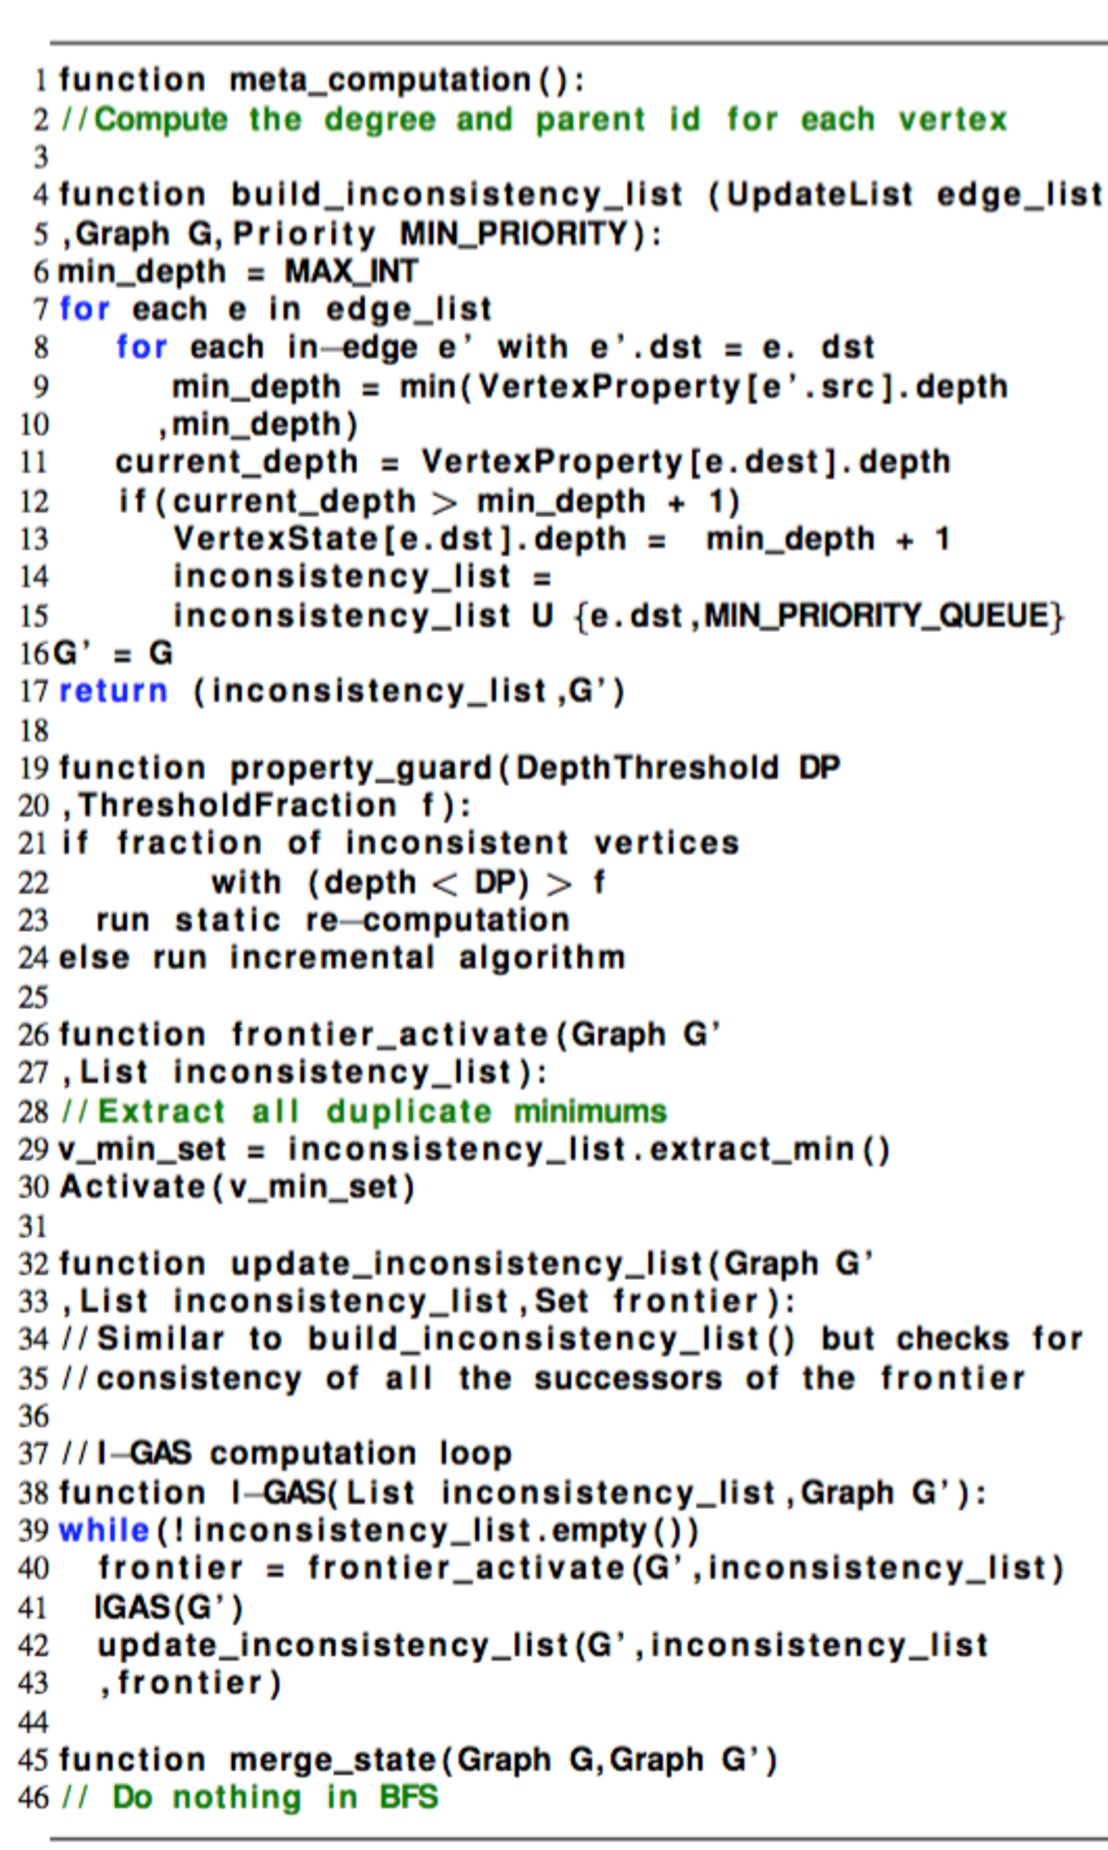
\includegraphics [width=\textwidth,height=0.85\textheight,keepaspectratio]{figures/BFS-inc.pdf}
\caption{\textbf{Stateful example:} Implementation of incremental BFS using EvoGraph APIs. }
\label{fig:BFS-inc}
%\vspace{-0.5\baselineskip}
%\vskip -3 mm
\end{figure}




\section{Case Studies}


\textbf{Stateful}. Detailed in Table \ref{tbl:table}, BFS is an example of a Stateful algorithm as it requires all the updates from one batch to be merged with the original graph before processing the next batch. Figure \ref{fig:bfs} illustrates the five computation phases of an incremental BFS. Phase I involves static computation of BFS depths from the source vertex (handled by GraphReduce~\cite{GraphReduce}) and metadata computation of properties such as degree and parent vertex id information for each vertex in the graph. In Phase II, vertices that have incorrect depth values~\cite{Ramalingam} after applying the current update batch are marked as inconsistent and added to a container with min-priority that is ordered by depth value. Phase III checks for any listed property to decide if the framework should run the incremental version or re-run the static recomputation algorithm. In BFS,  we use vertex depth as the property and check if the fraction of inconsistent vertices with depth values below a certain threshold (e.g., 2) have crossed certain limit. In Phase IV, EvoGraph fixes the inconsistency in the vertices of the graph in the order of their minimum depth values, as described in the algorithm by Ramalingam and Reps~\cite{Ramalingam}. Therefore, in each iteration of I-GAS loop, inconsistent vertices with the minimum depth value (can be multiple vertices) are activated and made consistent; and the inconsistency list is updated. Phase V is trivial as the vertex states are shared and hence do not require merging. Figure \ref{fig:BFS-inc} shows the BFS implementation in EvoGraph.



\textbf{Partially Stateless}. Shown in Table \ref{tbl:table} and Figure \ref{fig:cc}, Connected Components (CC) is a partially stateless algorithm because only deletions are required to be merged with  $G$.  For deletions we need to re-run the static algorithm and there are few proposed optimizations~\cite{CC},~\cite{CC_new} to eliminate false delections so that a component will not be broken. Phase I calculates the static version of connected component. In Phase II, EvoGraph builds the inconsistent graph $G'$ with vertex ids as the component labels in the original graph, and for each edge insertion in $G$ it adds an edge in $G'$ if the endpoints of the edge belong to different components. $G'$ is also known as \textit{component graph}~\cite{CC}. Phase III checks for the fraction of inconsistent vertices that belong to disjoint components. Phase IV runs static connected components algorithm on $G'$. Note that EvoGraph has successfully reduced the incremental problem in $G$ to a static problem in $G'$. Finally, Phase V relabels the vertices in $G$ from the computed component labels in $G'$. Figure \ref{fig:CC-inc} shows the CC implementation in EvoGraph.

\begin{figure}[!t]
%\vskip -3 mm
\centering
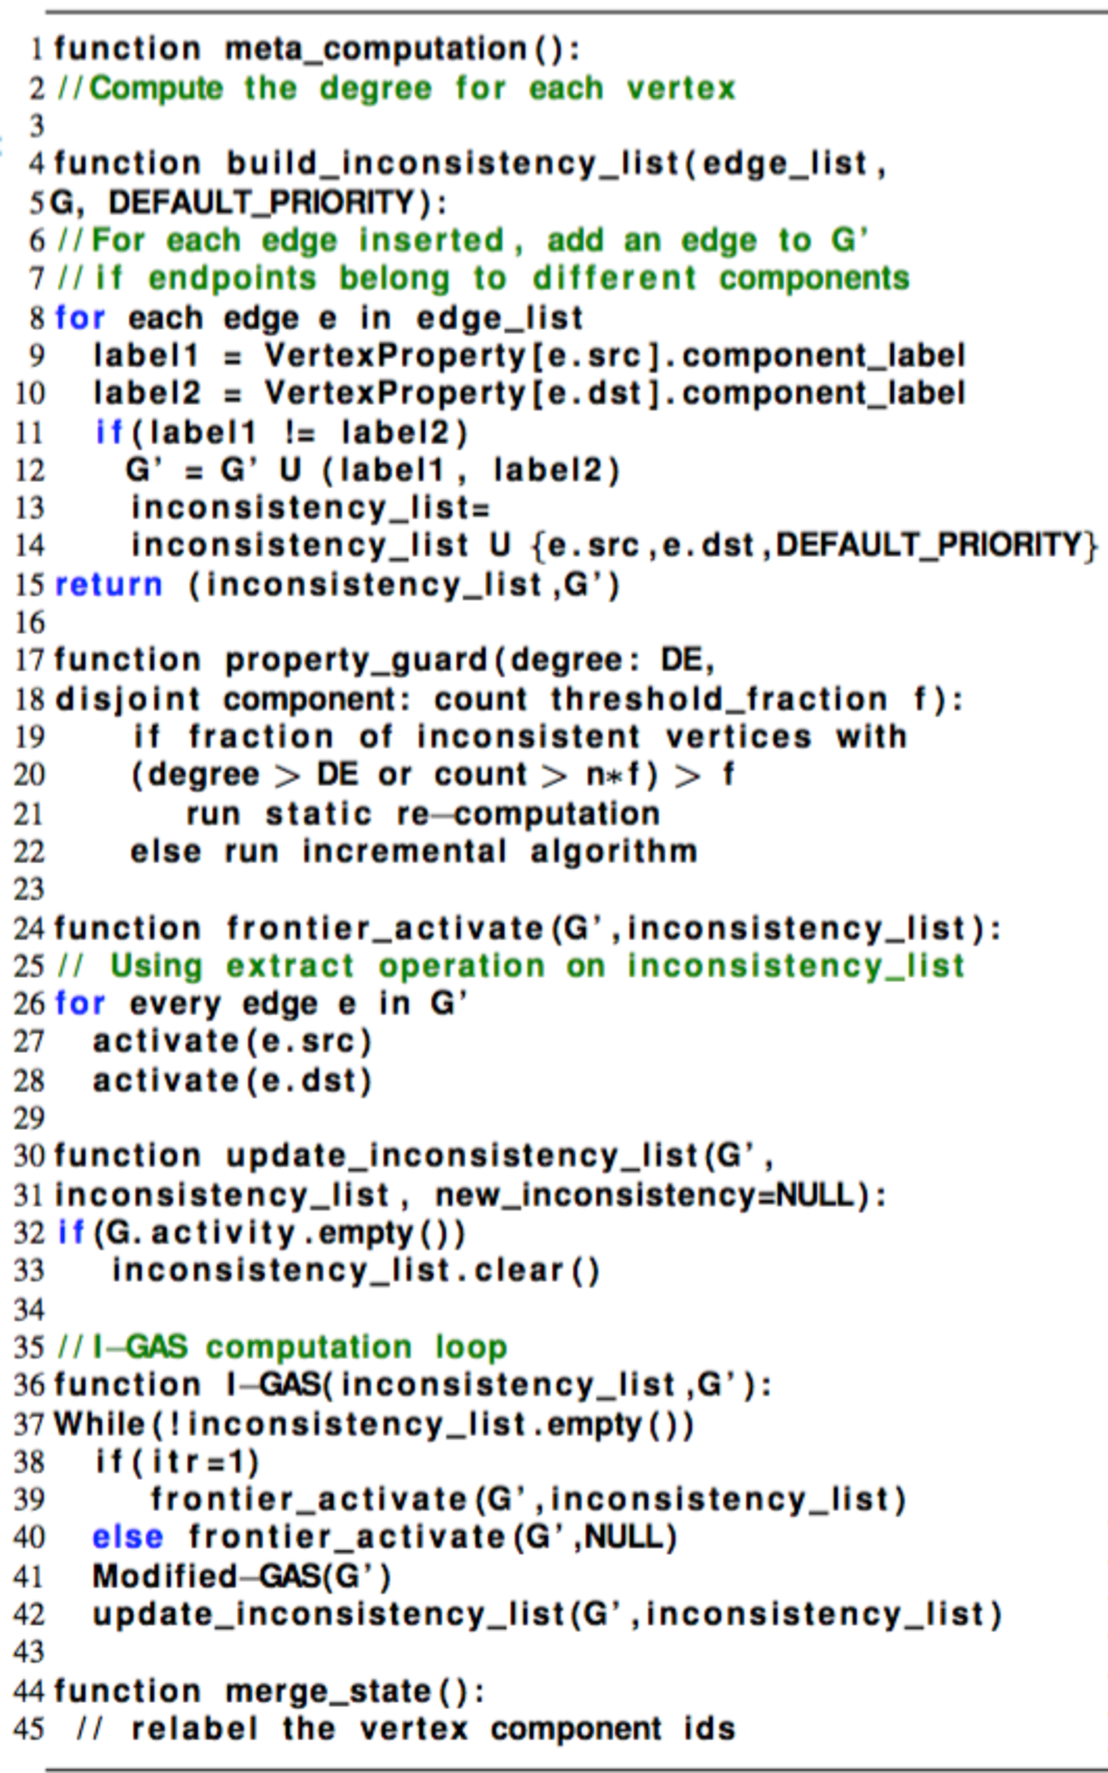
\includegraphics [width=\textwidth,height=0.85\textheight,keepaspectratio]{figures/CC-inc.pdf}
\caption{\textbf{Partially Stateless example:} Implementation of incremental Connected Components using EvoGraph APIs. }
\label{fig:CC-inc}
%\vspace{-0.5\baselineskip}
%\vskip -3 mm
\end{figure}

\textbf{Fully Stateless}. As illustrated in Table \ref{tbl:table}, Triangle Counting (TC), which measures the total number of closed triangles in a graph representing small-worldness of a graph, is a fully stateless algorithm because both insertions and deletions from an update batch are not required to be merged with the original graph before processing the next batch. Phase I computes the static version of the algorithm and the degree property for each vertex (metadata computation). In Phase II, EvoGraph marks the endpoints of every edge inserted or deleted and their respective neighboring vertices as inconsistent. Then it builds the inconsistent graph $G'$ with edges incident on every inconsistent vertex. Phase III checks for the fraction of inconsistent vertices in $G$ that have degree above certain threshold. Phase IV is similar to that in CC, activating all the vertices in $G'$ and then running the static algorithm on $G'$. Note that EvoGraph has again successfully reduced a fully dynamic (having both insertions and deletions) problem in $G$ to a static problem in $G'$. Finally, Phase V updates the triangle counts and the degree info in $G$ using the corresponding computed values in $G'$. Users can also implement a Bloom Filter version of the incremental algorithm for fast membership queries as shown in~\cite{CCof}. Figure \ref{fig:TC-inc} shows the TC implementation in EvoGraph.


\begin{figure}[!t]
%\vskip -3 mm
\centering
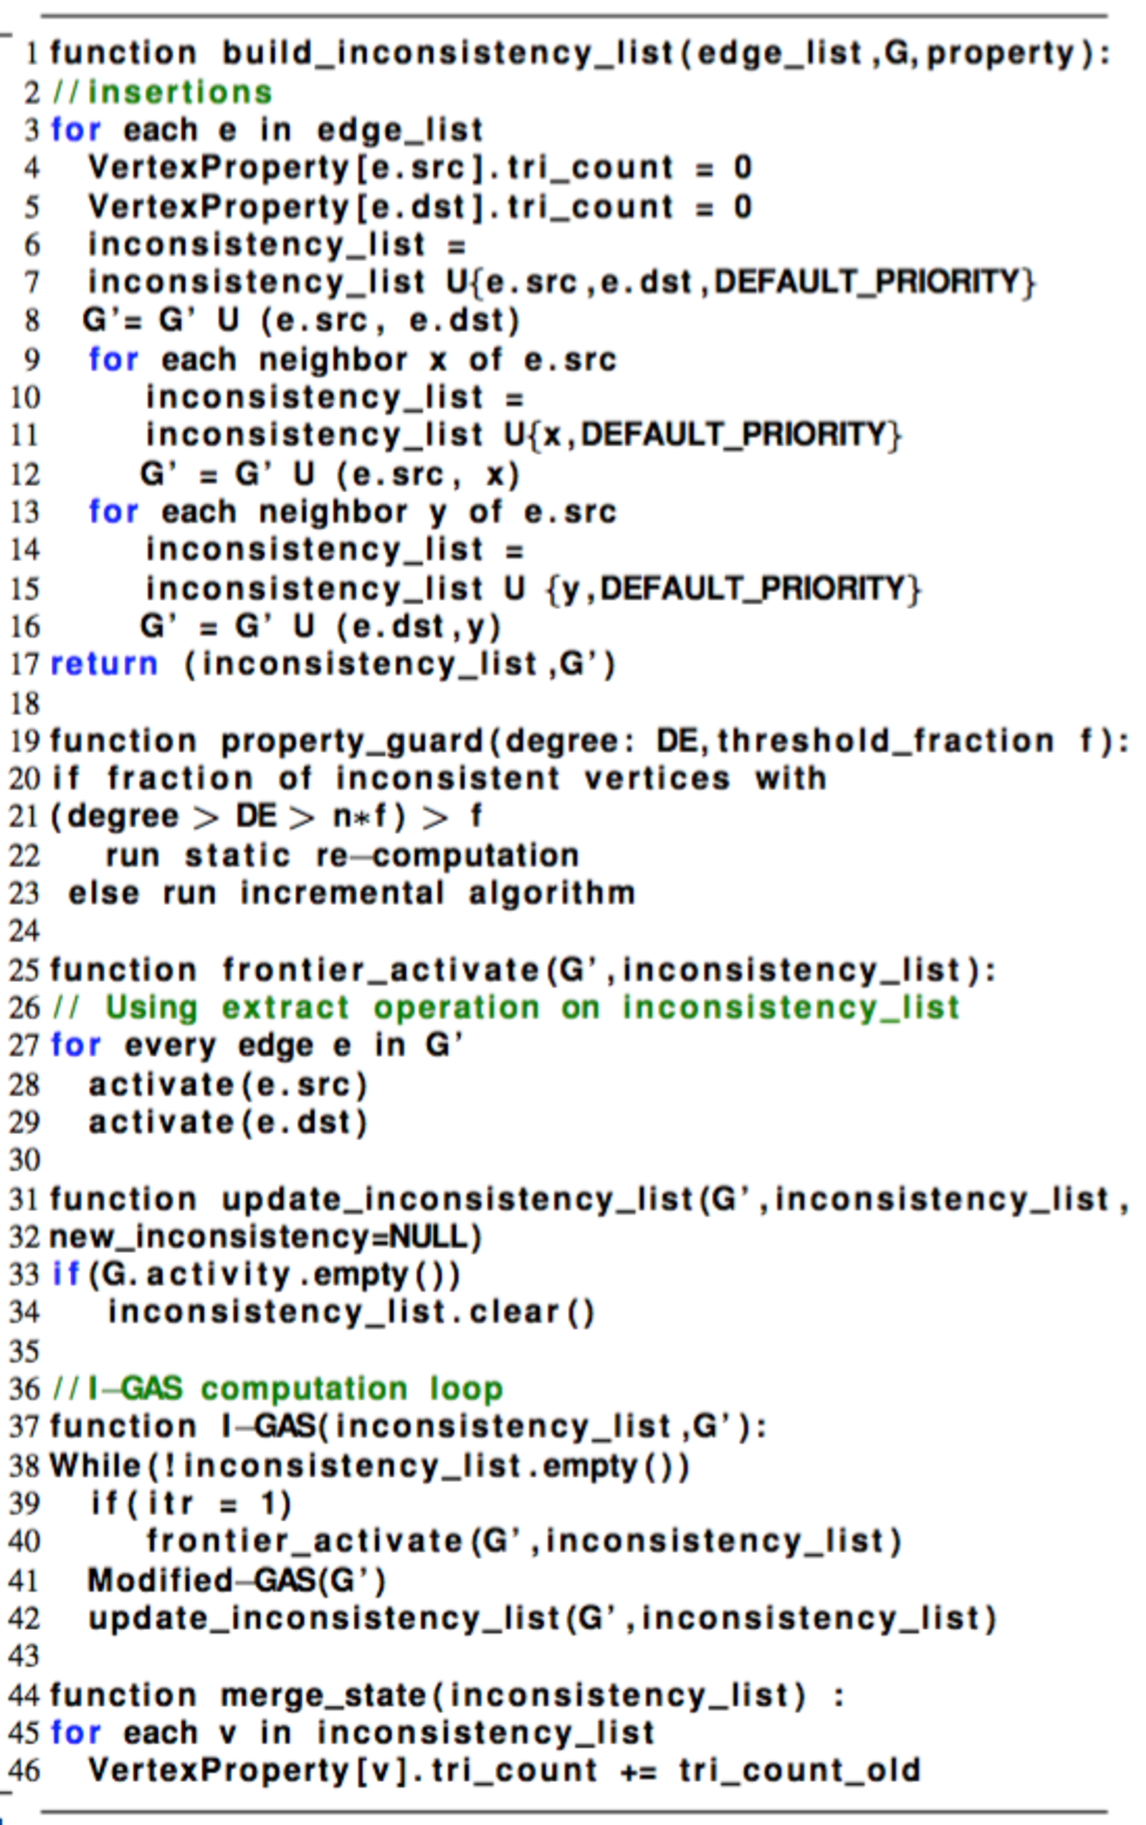
\includegraphics [width=\textwidth,height=0.85\textheight,keepaspectratio]{figures/TC-inc.pdf}
\caption{\textbf{Fully Stateless example: }Implementation of incremental Triangle Counting using EvoGraph APIs. }
\label{fig:TC-inc}
%\vspace{-0.5\baselineskip}
%\vskip -3 mm
\end{figure}

\section{Experimental Evaluation}
\subsection{Experimental Setup}

\textbf{Evaluation Platform}. We evaluate EvoGraph on a typical heterogeneous HPC node equipped with 12-core Intel Xeon  X5660 processors running at 2.8 GHz with 12 GB of DDR3 RAM, and one attached NVIDIA Tesla K40c GPU with 15 SMX multiprocessors and 12 GB GDDR5 RAM. The Kepler GPU is enabled with CUDA 7.0 runtime and the version 352.79 driver, while the host CPU is running Fedora version 20 with kernel v.3.11.10-301 x86. We use GraphReduce~\cite{GraphReduce} and STINGER~\cite{stinger},~\cite{CC},~\cite{CCof} for performance comparisons. All the runs are compiled with the highest optimization level flag. Updates are provided in batches to EvoGraph and STINGER where each batch size can range from 100,000 up to one million. For all three algorithms, the batch consists of 99\% edge insertions and 1\% deletions. The endpoints of the edges used for batch updates are generated randomly.

\begin{table}[]%\footnotesize
\centering
\caption{Graph Datasets Under Evaluation}
\label{dataset}
\begin{tabular}{|c|c|c|c|}
\hline
Graph Dataset & Type & \#Vertices & \#Edges \\ \hline
hollywood-2009 & real world & 1,139,905 & 113,891,327 \\ \hline
indochina-2004 & real world & 7,414,866 & 194,109,311 \\ \hline
ljournal-2008 & real world & 5,363,260 & 79,023,142 \\ \hline
kron\_g500-logn21 & real world & 2,097,152 & 182,082,942 \\ \hline
uk-2002 & real world & 18,520,486 & 298,113,762 \\ \hline
G19D16 & synthetic & 524,288 & 8,388,608 \\ \hline
G20D16 & synthetic & 1,048,576 & 15,700,394 \\ \hline
G21D16 & synthetic & 2,097,152 & 31,771,509 \\ \hline
\end{tabular}
%\vspace{-0.5cm}
\end{table}

\textbf{Graph Dataset}. For evaluating the performance of EvoGraph, we use a mix of real-world and synthetic datasets. Their graph properties are shown in Table \ref{dataset}. The five real-world datasets are from University of Florida Sparse Matrix Collection~\cite{UFL}. The synthetic datasets are obtained from the Graph500 RMAT data generator~\cite{graph500} using scale 19, 20 and 21 with average degree of 16 per vertex, labeled as G19D16, G20D16, and G21D16 respectively.

\textbf{Evaluated Algorithms}. Three widely used graph algorithms are evaluated, including Triangle Counting (fully-stateless), Connected Components (partially-stateless) and Breadth-First Search (stateful), to cover the three classes of algorithm patterns (Section 4.4). Algorithms requiring undirected graphs as inputs (e.g., CC) are stored as pairs of directed edges.

\begin{figure}[!t]
%\vskip -3 mm
\centering
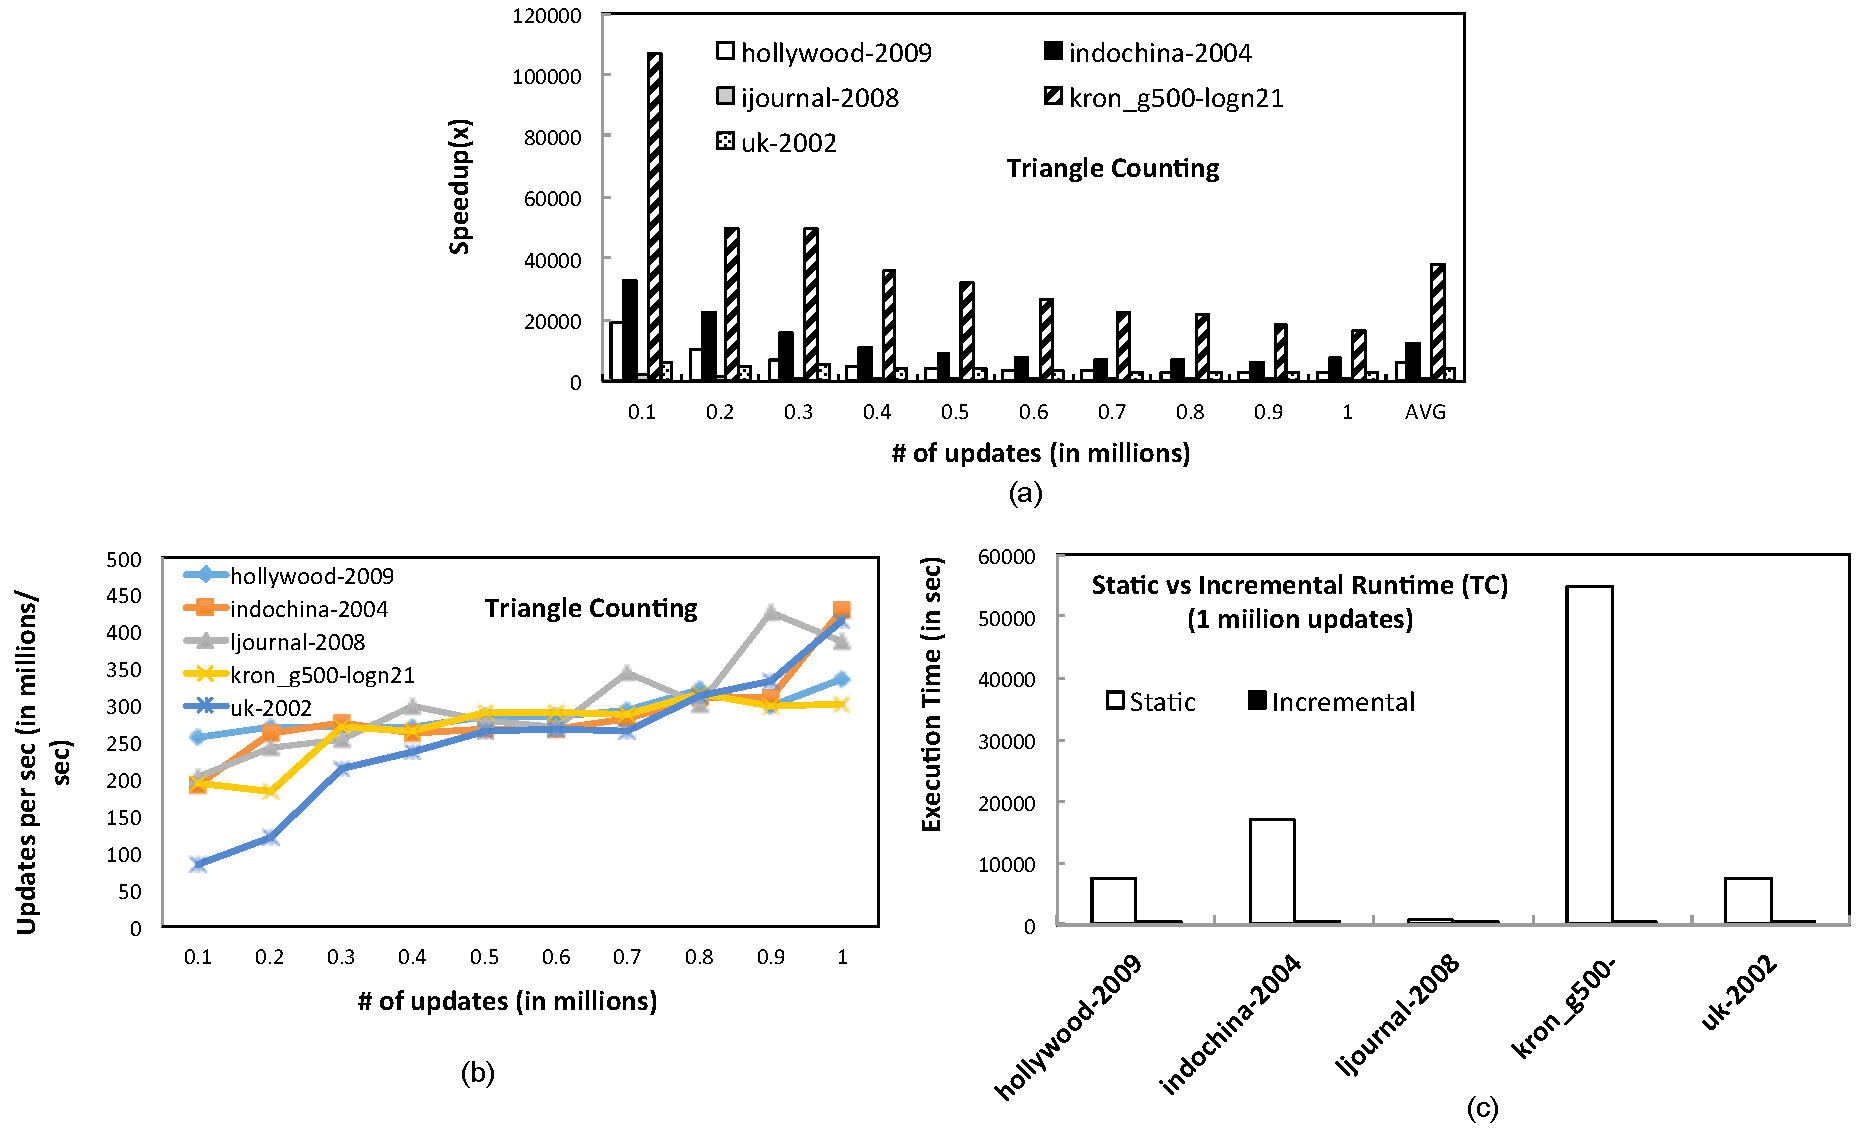
\includegraphics [width=1\columnwidth]{figures/exp3.pdf}
\caption{TC: (a) EvoGraph's speedup over the static computation using GraphReduce; (b) Update Rate that EvoGraph achieves; (c) For 1 million updates, EvoGraph vs. Static Runtime using GraphReduce. }
\label{fig:exp3}
%\vspace{-0.5\baselineskip}
%\vskip -3 mm
\end{figure}

\begin{figure}[!t]
%\vskip -3 mm
\centering
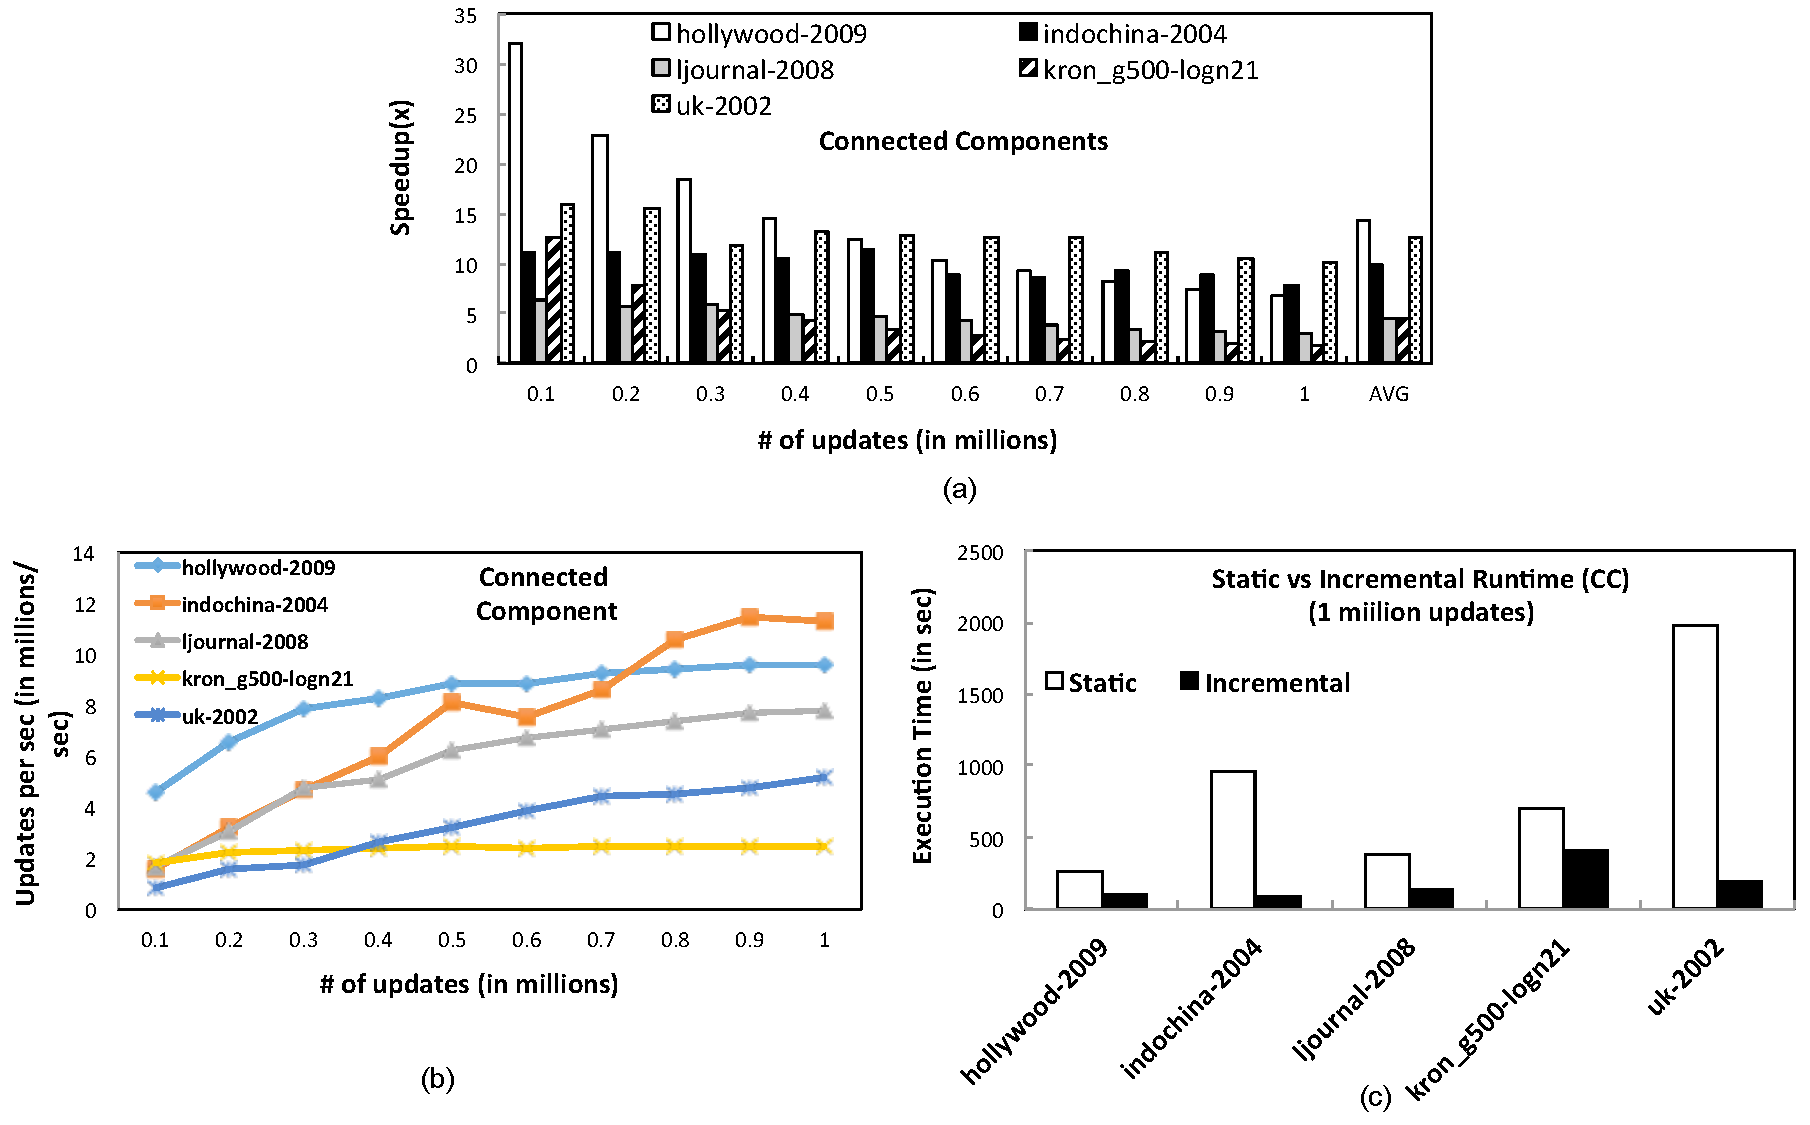
\includegraphics [width=1\columnwidth]{figures/exp2.pdf}
\caption{CC: (a) EvoGraph's speedup over the static computation using GraphReduce; (b) Update Rate that EvoGraph achieves; (c) For 1 million updates, EvoGraph vs. Static Runtime using GraphReduce. }
\label{fig:exp2}
%\vspace{-0.5\baselineskip}
%\vskip -3 mm
\end{figure}

\begin{figure}[!t]
%\vskip -3 mm
\centering
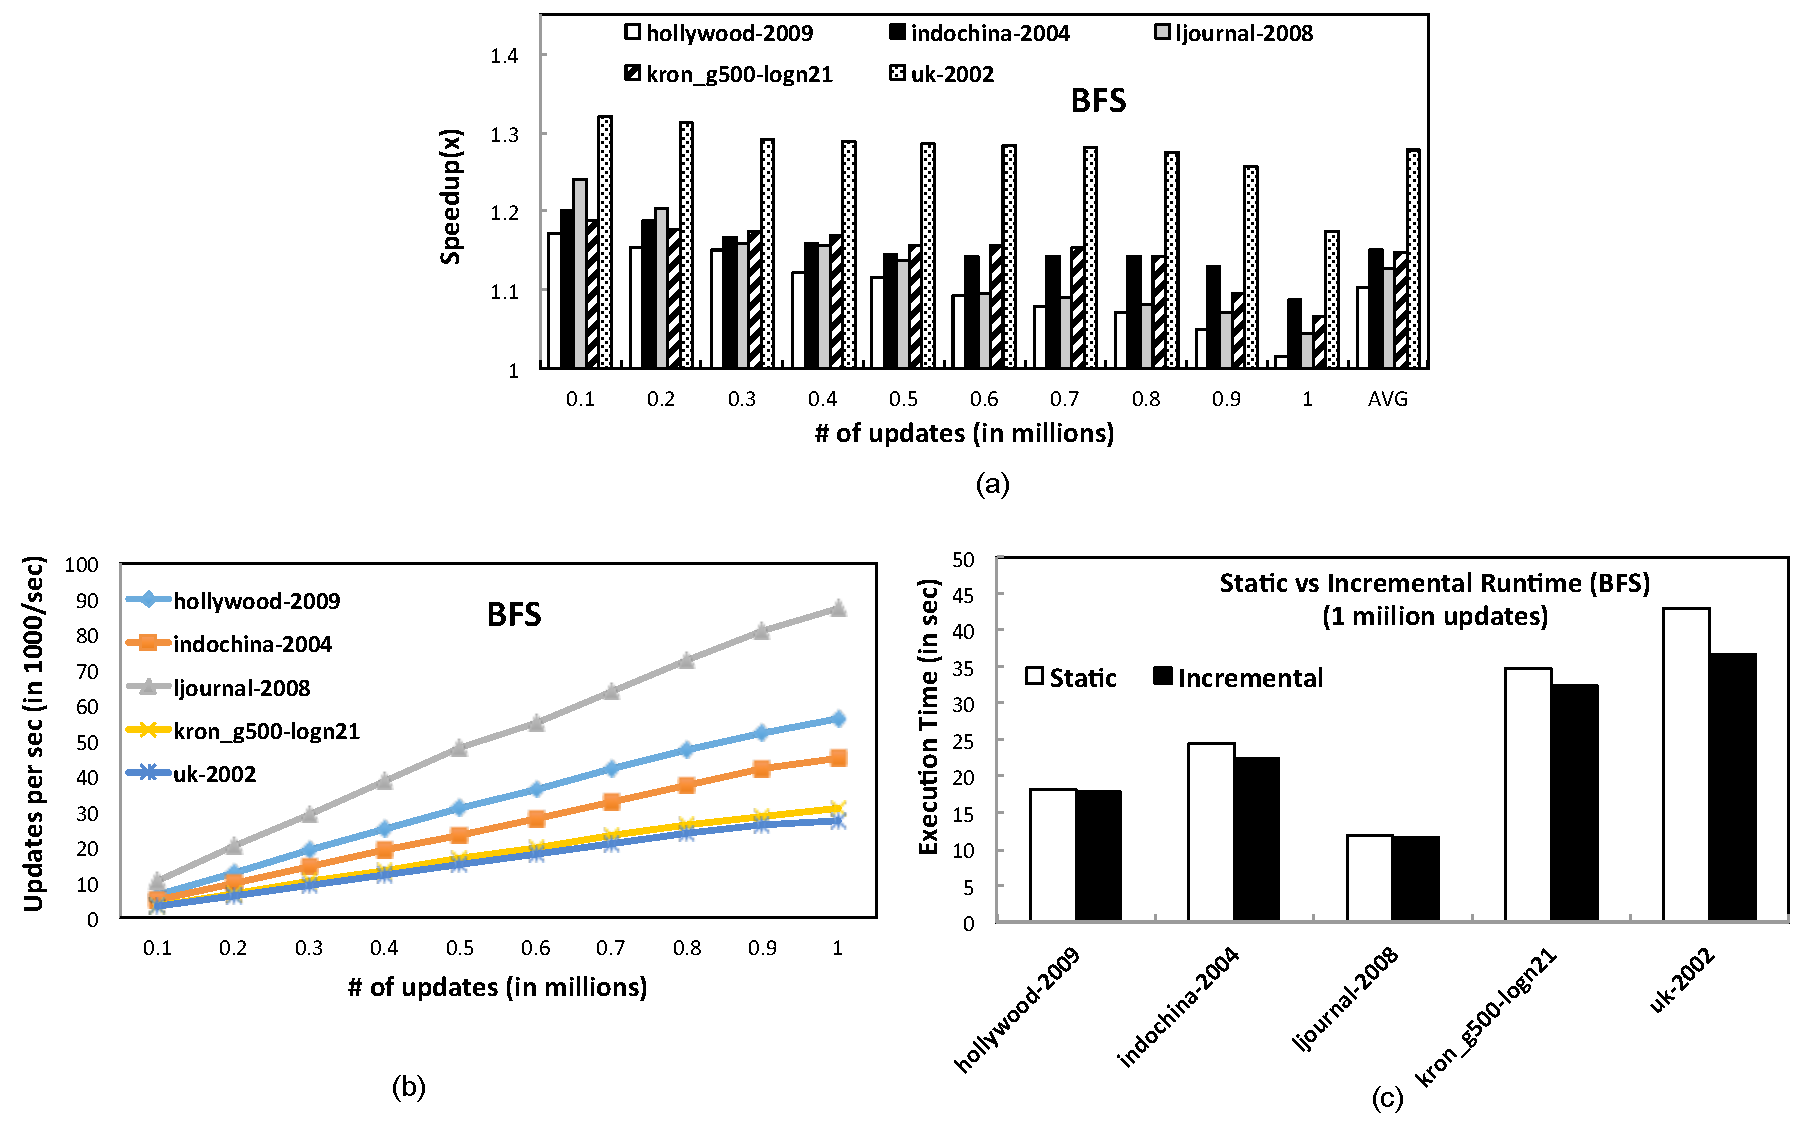
\includegraphics [width=1\columnwidth]{figures/exp1.pdf}
\caption{BFS: (a) EvoGraph's speedup over the static computation using GraphReduce; (b) Update Rate that EvoGraph achieves; (c) For 1 million updates, EvoGraph vs. Static Runtime using GraphReduce. }
\label{fig:exp1}
%\vspace{-0.5\baselineskip}
%\vskip -3 mm
\end{figure}



\subsection{EvoGraph Vs. Static Recomputation}


To process evolving graphs, the state-of-the-art GPU frameworks suchs as GraphReduce and Cusha, which only process static graphs, have to follow a store-and-static-compute model, repeatedly running static graph computation on the “snapshots” of the evolving graph. Here we showcase the benefits of incremental graph analytics (EvoGraph) over such offline static recomputation using GraphReduce~\cite{GraphReduce}. Figure \ref{fig:exp3}(a) , \ref{fig:exp2}(a) and  \ref{fig:exp1}(a) show that  EvoGraph achieves an average performance improvement of 12278x, 9.13x and 1.16x over GraphReduce across all the datasets for TC, CC and BFS, respectively, with the update batch size going as high as 1 million updates. Figure  \ref{fig:exp3}(b), \ref{fig:exp2}(b) and \ref{fig:exp1}(b) demonstrates that EvoGraph is able to achieve up to 429 million updates/sec.  Figure \ref{fig:exp3}(c), \ref{fig:exp2}(c) and  \ref{fig:exp1}(c) compares the incremental and static runtime performance for TC, CC and BFS for a batch size of 1 million updates. It clearly demonstrates the performance benefit using EvoGraph for incremental graph processing. The tremendous performance improvement achieved by EvoGraph is due to (i) the use of incremental computation in the I-GAS execution model to compute the vertex states for only the inconsistent set of vertices, as opposed to executing the algorithm on the entire input graph; (ii) asynchronous mode and deep copy operations between host and device leveraging CUDA Streams and \textit{Hyper-Qs} to keep both compute and memory-copy engines occupied simultaneously; (iii) concurrent static and incremental graph processing via time and space sharing on GPU by Context Merging (Section 4.2.4), resulting in substantial reduction in context-switching overhead and GPU core idling. Furthermore, we can draw key inferences as to how the performance of incremental execution varies with algorithm type, update batch size and input graph size. 



\subsection{Sensitivity Analysis}

\textbf{Effect of graph algorithm}. Figure \ref{fig:exp3}, \ref{fig:exp2} and  \ref{fig:exp1} show that the maximum speedup achieved by EvoGraph over static recomputation occurs with TC (fully stateless), followed by CC (partially stateless) and then BFS (stateful). Also, the relative runtime performance of TC is the highest compared to CC and BFS. Additionally, the average system throughputs achieved across all graph algorithms for a batch size of 1 million updates are 372 million, 7.3 million and 50K updates/sec for TC, CC and BFS, respectively. This drastic difference in performance across different merge patterns is because the fraction of the graph that becomes inconsistent after applying an update batch as the I-GAS loop unfolds increases in the order of fully-stateless, partially-stateless, and stateful. In other words, fully-stateless or partially-stateless algorithms only affect the graph locally, so the incremental runtime is bounded by the size of the update batch. On the contrary, stateful algorithms like BFS calculate a global property (e.g., vertex depth), so the incremental computation affects a larger portion of the graph and hence achieves lower speedup.  Furthermore, during the State-Merging phase of incremental BFS, the new update batch is applied or merged with the current static version which in turn is copied back to the GPU. This incurs a large data transfer overhead, whereas for TC and CC the data transfers are of the order of the update batch size, keeping the memcpy time small. 

\textbf{Effect of update batch size}. Shown in Figure \ref{fig:exp3}(a)-\ref{fig:exp1}(a), the speedup falls as the update batch size increases because of the increasing problem size. We also observe that both the runtime (because of decreasing speedup) and update rate increases with the batch size (Figure \ref{fig:exp3}(a)-\ref{fig:exp1}(a)), which implies that the decrease in speedup changes slower with respect to dramatic update rate increases for larger batches.


\textbf{Effect of input graph size}. Finally, from Figure \ref{fig:exp3}(b)-\ref{fig:exp1}(b)  we can observe that BFS's throughput increases with the batch size a lot faster for smaller graphs (e.g., ijournal-2008) than for the larger ones (e.g., uk-2002). This happens because for updates affecting a particular BFS level, the cost of incremental computation increases with the size of the inconsistent subgraph which in turn is proportional to the size of the input graph. On the other hand, the update rates of CC and TC show no correlation with the input size as the graph properties under consideration are local or semi-local, whose performance is more likely dependent on properties such as number of disjoint components and vertex degree.

\begin{figure}[!t]
\centering
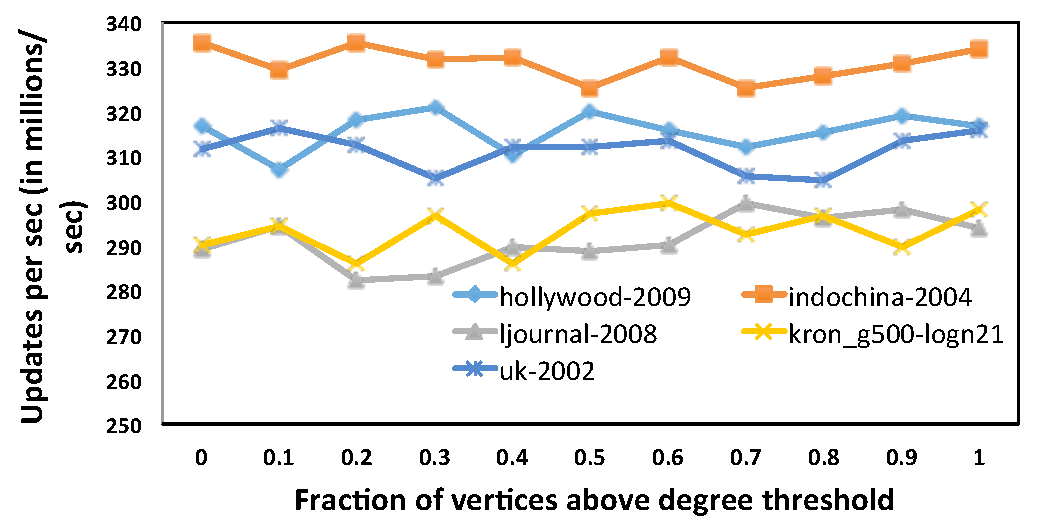
\includegraphics [width=0.75\textwidth,height=\textheight,keepaspectratio]{figures/prop1.pdf}
\caption{Impact of vertex degree property on the update rate of Triangle Counting algorithm.}
\label{fig:prop1}
%\vspace{-1.2\baselineskip}
\end{figure}

\begin{figure}[!t]
\centering
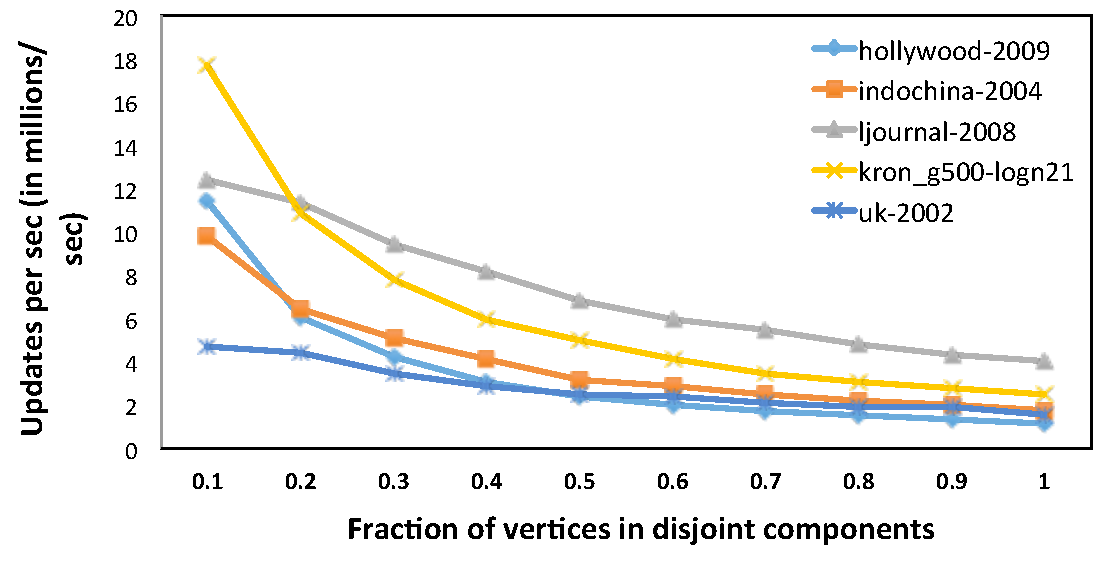
\includegraphics [width=0.75\textwidth,height=\textheight,keepaspectratio]{figures/prop2.pdf}
\caption{Impact of disjoint components property on the update rate of Connected Components algorithm.}
\label{fig:prop2}
%\vspace{-1.2\baselineskip}
\end{figure}

\begin{figure}[!t]
\centering
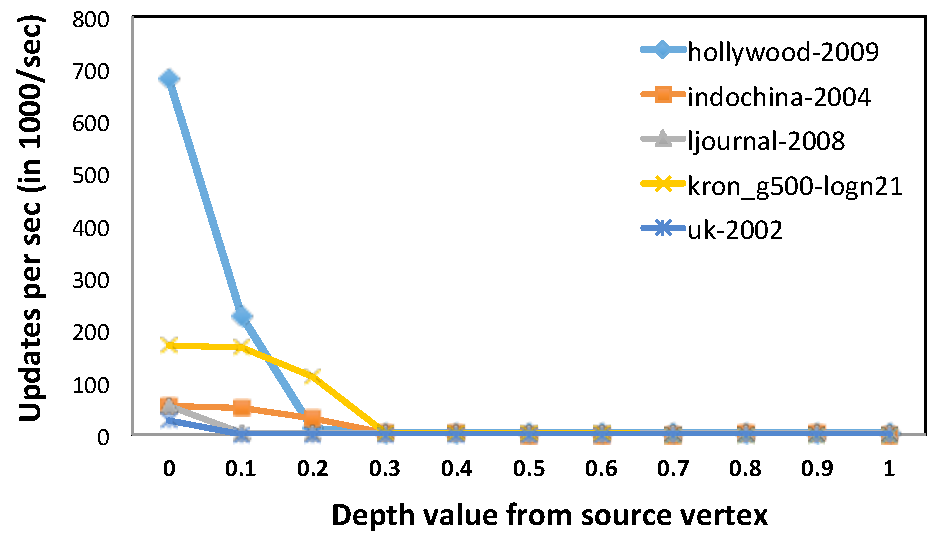
\includegraphics [width=0.70\textwidth,height=\textheight,keepaspectratio]{figures/prop3.pdf}
\caption{Impact of vertex depth property on the update rate of Breadth First Search algorithm.}
\label{fig:prop3}
%\vspace{-1.2\baselineskip}
\end{figure}



\subsection{Performance Implications of Graph Properties}

Now we evaluate how properties of the inconsistent vertices from a given update batch affect the average runtime and throughput of incremental graph processing. For demonstration, we have chosen specific graph property for each of the three algorithms: vertex degree for TC, vertices with disjoint components for CC,  and vertex depth from the source for BFS. The rationale behind choosing these properties is that they play an essential role in the static graph algorithms that we are comparing against.  

\textbf{Triangle Counting (Vertex Degree)}:  Figure \ref{fig:prop1}(a) shows the change in the update rate for TC versus the fraction of updates (insertions and deletions) affecting vertices with degree greater than a certain threshold (e.g. 1900 for Hollywood graph). We vary the fraction of inconsistent vertices with degree higher than the threshold degree in a given update batch and then evaluate its effect on the incremental runtime and the update rate. We can observe that the degree property does not have a dramatic effect on the update rate for TC. This is because TC is a stateless algorithm for both insertions and deletions to the graph, and the size of the sub-graph $G'$ created in Phase II (see Table \ref{tbl:table}), and thus the incremental runtime is independent of the vertex degree. Therefore, the update rate remains relatively constant even when more edges are inserted and/or deleted near high degree vertices or supernodes. 

\textbf{Connected Components (Disjoint Components)}: Figure \ref{fig:prop2}(b) shows that the update rate for CC decreases as the fraction of edges inserted (whose endpoints belong to different components in the original graph) is increased, with a maximum slowdown of 10.2x across all the datasets. This happens because the endpoints of an edge falling in the same component results in a self-edge in the component graph and ignored by EvoGraph. On the contrary, if the endpoints are in different components implying that there is a corresponding edge in the component graph G'. From Table \ref{tbl:table}, EvoGraph reduces incremental CC on G to static CC processing on G' and increasing the number of vertices with disjoint components proportionately increases the size of G', and subsequently increasing the incremental processing time.

\textbf{BFS (Vertex Depth)}:  Figure \ref{fig:prop3}(c) shows that increasing the fraction of vertices with depth below a given threshold (MAX\_DEPTH/4 in our case) causes a sharp decline in the update rate. This slowdown comes from more insertions and deletions on these lower-depth vertices closer to the root vertex, which results in the I-GAS loop making a much larger portion of the graph inconsistent with each increment. The maximum slowdown (max to min ratio of the update rate) across all datasets is 213x which can lead to dramatic system performance degradation and hence motivates our \textit{property guard} heuristic which we discuss next.


\begin{figure}[!t]
\centering
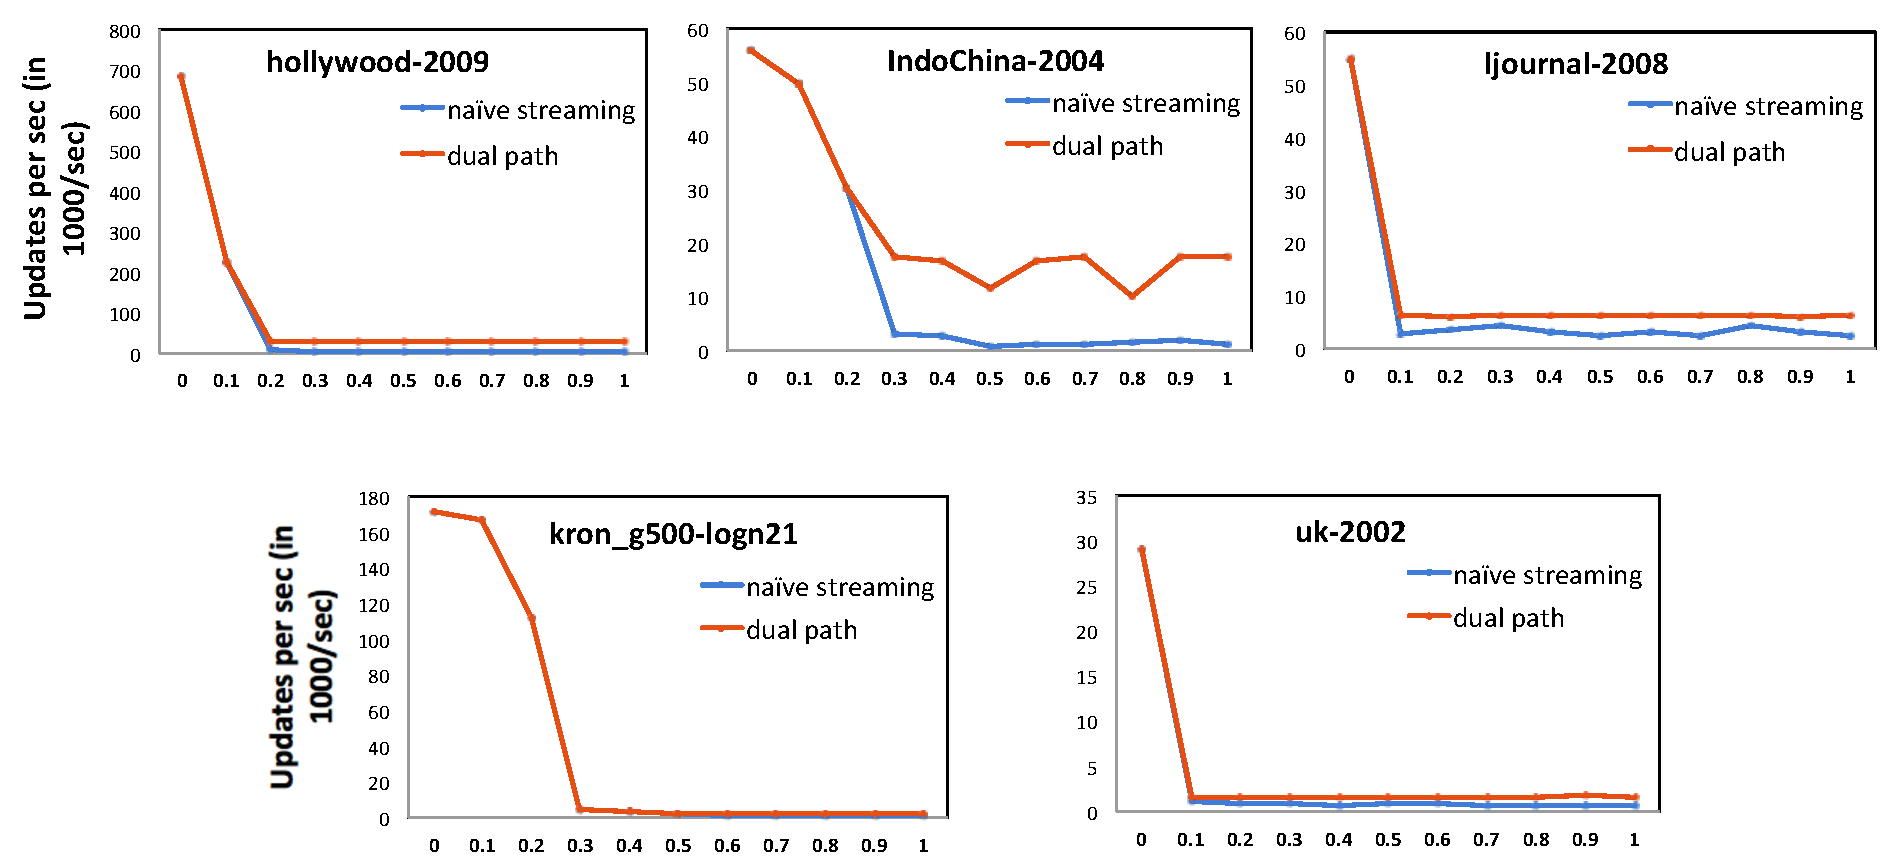
\includegraphics [width=\textwidth,height=\textheight,keepaspectratio]{figures/prop_guard.pdf}
\caption{Property-guard heuristic vs. naive streaming in incremental BFS using vertex depth property for five graph inputs. The x-axis represents the fraction of vertices below depth threshold of MAX\_DEPTH/4. }
\label{fig:five}
%\vspace{-1.2\baselineskip}
\end{figure}

\textbf{Property-Guard Heuristic}: In these sets of experiments we show how EvoGraph uses property information and adapts to situations where the incremental processing performs worse than static recomputation. Figure \ref{fig:five} shows that the performance of incremental BFS for naive streaming without considering the property information of the current update batch falls relative to static processing beyond a threshold fraction of vertices with depth threshold below MAX\_DEPTH/4. For Hollywood, Indochina, Ljournal, KronLogn21 and UK-2002 this threshold fractions are 0.2, 0.3, 0.1, 0.5 and 0.1 respectively. As discussed in the previous section, this degradation in incremental performance is because a larger number of updates to these lower-depth vertices results in a large portion of the graph becoming inconsistent and hence significant increase in processing time. In phase III, EvoGraph analyzes the current update batch for the depth threshold and if the batch has a fraction of vertices beyond certain thresholds, instead of proceeding to I-GAS incremental execution, processes the update batch with static recomputation ensuring the worst-case performance has the same lower bound as static recomputation. We achieve a maximum speedup of 18.4x, using this heuristic, compared to a naive streaming approach (Indochina). 

\subsection{EvoGraph VS. STINGER}
Figure~\ref{fig:stinger} shows the comparison between the update rate for EvoGraph vs. STINGER [29] for TC and CC. Note that for fairness data transfer time between host and GPU has been included for EvoGraph computation while STINGER is not subject to such overhead. Across all 3 synthetic datasets STINGER shows a max update rate of 2.1 million versus 488 million updates/sec with EvoGraph for the S19D16 case, a 232.4x increase in throughput. EvoGraph also shows better scalability as batch size increases because of (1) the massive parallelism offered by thousands of cores of GPU that is sufficient to overcome the substantial overheads from the large data movement over PCIe, (2) EvoGraph’s hybrid data structure of edge-list for incremental updates and compressed matrix format for static versions of the graph. STINGER uses edge-list based data structures for both the static and incremental graph processing, which results in faster data structure update time but slower traversal time due to list traversal. EvoGraph’s hybrid data structure thus enables faster updates (via the edge-list) as well as fast static computation (via compressed matrix format). 

\begin{figure}[!t]
\centering
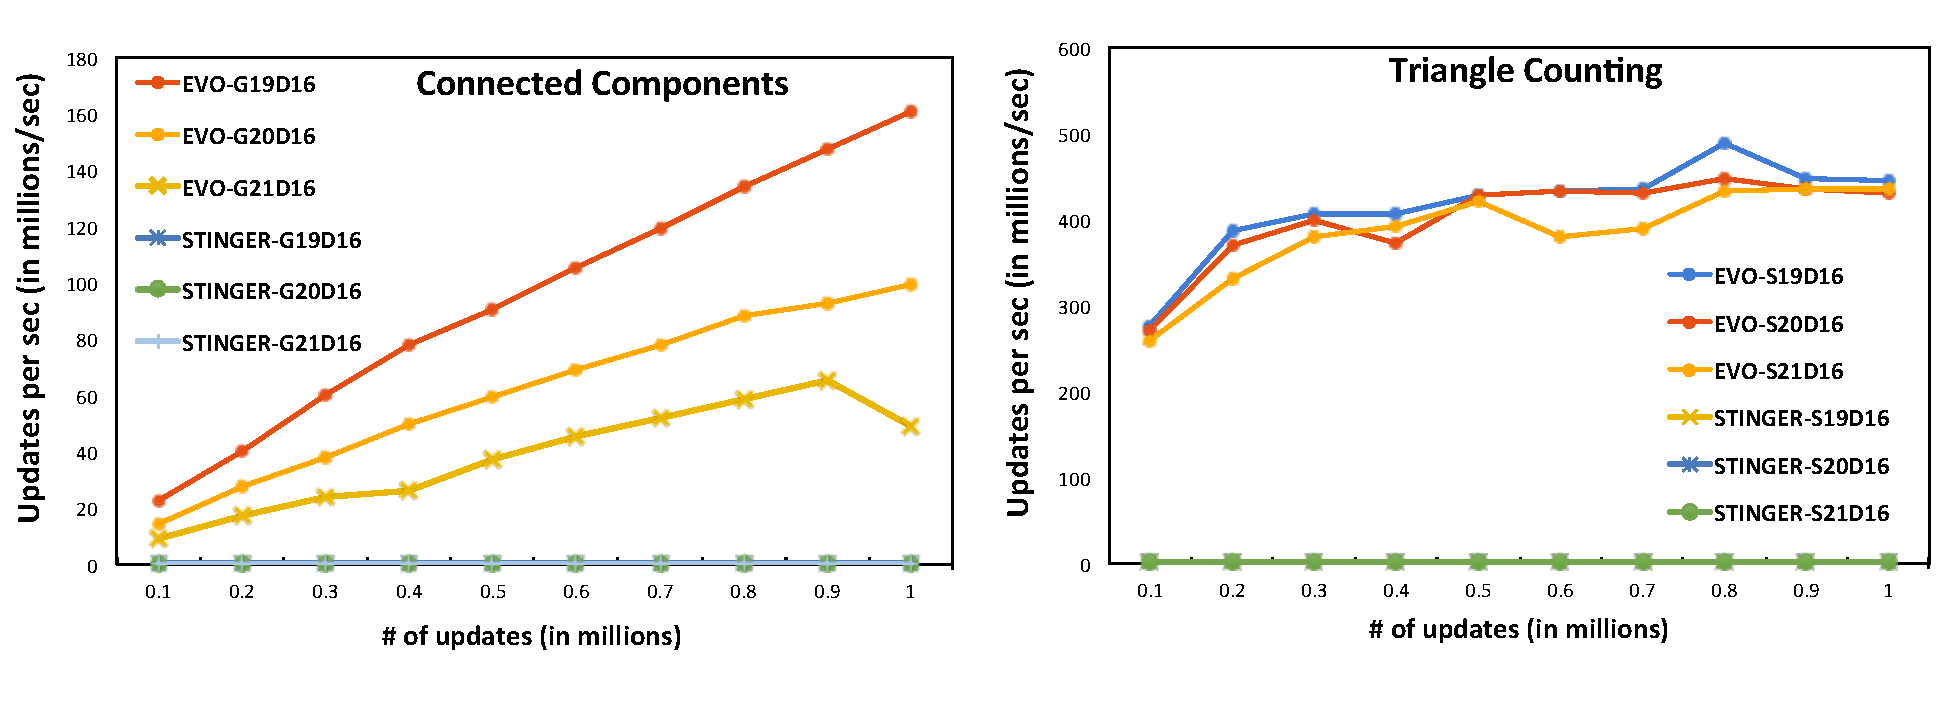
\includegraphics [width=\textwidth,height=\textheight,keepaspectratio]{figures/exp_stinger.pdf}
\caption{EvoGraph vs STINGER throughput comparison for (a) Connected Components and (b) Triangle Counting.}
\label{fig:stinger}
%\vspace{-1.5\baselineskip}
\end{figure}
\subsection{Discussion} 
Experiments demonstrate that (1) EvoGraph’s incremental approach to process time-evolving graphs on GPUs, combined with its asynchronous and deep memory copy operations on separate CUDA streams leveraging the multiple hardware queues (Hyper-Qs) in GPUs; and context merging of various static and incremental graph algorithm for better GPU utilization, can achieve dramatic speedups of up to 12278x over traditional store-and-static-recompute model with a maximum system throughput of 429 million updates/sec across several real-world and synthetic graphs. (2) The  graph algorithm type, based on their merge pattern,  can have a dramatic impact on the update rate achieved with a fully stateless (TC) and stateful (BFS) algorithm achieving an average throughput of 50K and 372 million updates/sec respectively with a batch of  1 million updates. (3) Vertex properties of an update batch investigated either do not affect the update rate, as in the case of vertex degree with TC, or can have a dramatic impact on the update rate, as in the case of vertex depth with BFS resulting in a maximum slowdown of 213x. The impact of such properties largely is related to the portion of the graph that is made inconsistent with each iteration. (4) The property-based dual path execution optimization in EvoGraph to choose between an incremental vs static run over a particular update batch can achieve up to 18.4x compared to naive streaming approach. (5) Leveraging the massive parallelism offered by thousands of cores of GPU and its hybrid data structure of edge-list for incremental updates and compressed matrix format for  static versions, EvoGraph achieves a speedup of upto 232.4x compared to STINGER.

\iffalse
\section{Related Work}

\textbf{Dynamic graph processing.} There are two broad categories of dynamic graphs processing (1) Offline processing of dynamic graphs that involves the generation, storing, and analysis of a sequence of versions or time-stamped snapshots of dynamic graphs for the calculation of some global graph property. (2) Online processing of dynamic graphs that  involve real-time, continuous query processing over streaming updates on the evolving graph. EvoGraph is a framework designed to address the later problem.
Chronos~\cite{chronos}, GraphScope~\cite{graphscope}, and TEG~\cite{teg} are some examples of the most recent work in offline dynamic graph processing. Chronos is a high-performance system that supports incremental processing on temporal graphs using a graph representation that places graph vertex data from different versions together leading to good cache locality. GraphScope proposes encoding for evolving graphs for community discovery and anomaly detection. 

\textbf{Real-time, continuous query processing.} This implies certain memory constraints that might not allow keeping multiple versions of the evolving graph. STINGER~\cite{stinger} defines an efficient data structure to represent streaming graphs that enables fast, real-time insertions and/or deletions to the graph. Several applications have been built using the STINGER graph representation like clustering coefficient [3] and connected components [4]. Unlike STINGER which uses a single data structure for both static and dynamic graph analysis, EvoGraph uses a novel hybrid data structure that allows for incremental computation on edge lists and a compressed format for static graph computation.  A key takeaway of these related work is that any existing algorithm that can be reduced to a GAS-based graph sub-problem can easily leverage EvoGraph to implement their incremental versions.


\textbf{Accelerator-based Graph Processing.}
Merrill et al.[29] present a parallelization of BFS tailored to the GPU’s requirement for large amounts of fine-grained BSP; they achieve an asymptotically optimal $O(|V | + |E|)$ work complexity. Duong et al. [14] conduct detailed GPU-based optimizations for PageRank and achieves significant speedup over a multi-core CPU implementation. Chapuis et al. [13] provide an algorithmic optimization solution to speedup all-pairs shortestpath (APSP) for planar graphs that exploits the massive on-chip parallelism available on GPUs. 	The GraphReduce~\cite{GR} framework can efficiently process graphs with large inputs and mutable edge values that can-not fit into the limited memories of discrete accelerators. The framework characterizes the memory buffers and then maps them to the different memory abstractions exposed by GPU, which at minimum, contain slow and fast memory~\cite{nemu}(e.g., host memory and GPU memory). 		 

Concerning frameworks for GPU-based graph processing, earlier work like Medusha~\cite{medusa} introduces some basic graph- centric optimizations for GPUs, offering a small set of user- defined APIs, but its performance is not comparable to the state-of-the-art low-level GPU optimizations. To address this issue, MapGraph~\cite{mapgraph} and VertexAPI~\cite{vertexapi} implement runtime-based programming frameworks with levels of performance that match those seen for low-level specific algorithm optimizations. MapGraph chooses among different scheduling strategies, depending on the size of the frontier and the adjacency lists for the vertices in the frontier. VertexAPI provides a GAS model-based GPU library, gaining high performance primarily from using the ModernGPU [6] library for load balancing and memory coalescing. CuSha~\cite{cusha} identifies the shortcomings of the state-of-the-art CSR- based virtual warp-centric method for processing graphs on GPUs and in response, proposes G-Shards and Concatenated Windows to address its performance inefficiency. All of the approaches above make the fundamental assumption that large graphs fit into GPU memory, a restriction that doesn't hold true for real-world graphs.

\textbf{Distributed graph processing.} Involves processing of large-scale graphs in a distributed fashion by making use of the combined memories of multiple machines to fit large graphs that don’t fit in a single machine. Pregel~\cite{pregel} provides a synchronous vertex-centric graph processing framework that is based on message passing. GraphLab~\cite{graphlab} provides a framework for machine learning and data mining while PowerGraph~\cite{powergraph} exploits the power-law vertex degree distribution for efficient data placement and computation. ASPIRE~\cite{aspire} adopts an asynchronous mode of execution with a relaxed consistency to improve the remote access latency. These project are complimentary to GraphIn, in that they could be used to implement the static component of GraphIn  computation while I-GAS can be leveraged to make these distributed frameworks more dynamic. 


\textbf{Out-of-Memory graph processing.} Out-of-Core graph processing has been concerned with CPU-based hosts processing graphs that do no fit into host memory. GraphChi~\cite{chi}, for instance, is based on a vertex-centric implementation of graph algorithms where graphs are sharded onto the SSD drives attached to the host. X-Stream~\cite{xstream} employ an edge-centric way to organize data for the GAS model. Totem~\cite{totem} offers a high-level abstraction for graph processing on GPU-based systems, by statically partitioning graphs into GPU and host memories, placing low- degree vertices on the host and high-degree vertices on the GPU. The approach improves performance if the graphs follow a power-law vertex degree distribution, and as graph size increases, only a fixed sub-graph able to fit in GPU memory will be processed, resulting in GPU underutilization and eventual CPU-based bottlenecks for graph processing. Green-Marl~\cite{green} is a Domain Specific Language (DSL) for efficient graph analysis on CPUs; its implementation is not amenable to many-core architectures.
Involves large-scale graph processing in a single machine with graphs that might not fit into host memory. GraphChi~\cite{chi},  X-Stream~\cite{xstream} are two of the recently proposed out-of-memory frameworks. GraphChi is based on a vertex-centric implementation of graph algorithms where graphs are sharded on SSD drives attached to the host while X-Stream uses an edge-centric way to organize data for GAS model. As EvoGraph is framework independent, these out-of-memory frameworks can be used as the static graph processing core for our framework.
\fi

\section{Chapter Summary}
This chapter presents EvoGraph, an accelerator-based high-performance incremental graph processing framework for processing time-evolving graphs. Technical advances offered by EvoGraph include: (1) an incremental variant of Gather-Apply-Scatter called I-GAS to compute graph properties only for the inconsistent subgraphs, (2) a user-tunable property-based optimization called property-guard for switching between I-GAS and static recomputation, and 3) deep memory copy operations via separate CUDA Streams and GPU context merging for improved asynchronous computation and communication performance. Evaluation on a variety of graph inputs and algorithms demonstrates that EvoGraph achieves a system throughput of up to 429 million updates/sec and a 232x speedup when compared to competitive frameworks like STINGER. Furthermore, the property-guard optimization of EvoGraph achieves a speed up of up to 18.4x over a naive streaming approach. Future work will look at extending EvoGraph to multi-node clusters and extreme-scale datasets.


